\documentclass[12pt]{article}
\usepackage[utf8]{inputenc}
\usepackage[russian]{babel}
\usepackage{amsmath}
\usepackage{amssymb}
\usepackage{MnSymbol}
\usepackage{wasysym}
\usepackage{mathtext}
\usepackage{mathenv}
\usepackage{listings}
\usepackage{color}
\usepackage{graphicx}
\usepackage{hyperref}
\usepackage{amssymb,amsfonts,amsmath,mathtext,cite,enumerate,float}
%\usepackage{algorithm}
\usepackage{float}
\usepackage[noend]{algpseudocode}
\usepackage[ruled,vlined]{algorithm2e}
\usepackage[a4paper, left=25mm, right=20mm, top=20mm, bottom=20mm]{geometry}
\usepackage{indentfirst}
\usepackage{epstopdf}

\DeclareGraphicsExtensions{.eps} 


\newtheorem{definition}{Определение}[section]
\newtheorem{remark}{Примечание}[subsection]
\newtheorem{suggest}[remark]{Соглашение}
\newtheorem{claim}[remark]{Утверждение}
\newtheorem{lemma}[remark]{Лемма}
\newtheorem{theorem}{Теорема}
\newtheorem{conseq}{Следствие}[theorem]
\newenvironment{Proof} 
	{\par\noindent{\bf Доказательство.}} 
	{\hfill$\blacksquare$}

\newenvironment{rusalgorithm}[1][htb]
  {\renewcommand{\algorithmcfname}{Алгоритм}
   \begin{algorithm}[#1]
  }{\end{algorithm}}



\definecolor{dkgreen}{rgb}{0,0.6,0}
\definecolor{gray}{rgb}{0.5,0.5,0.5}
\definecolor{mauve}{rgb}{0.58,0,0.82}

\lstset{frame=tb,
  language=Java,
  aboveskip=3mm,
  belowskip=3mm,
  showstringspaces=false,
  columns=flexible,
  basicstyle={\small\ttfamily},
  numbers=none,
  numberstyle=\tiny\color{gray},
  keywordstyle=\color{blue},
  commentstyle=\color{dkgreen},
  stringstyle=\color{mauve},
  breaklines=true,
  breakatwhitespace=true
  tabsize=3
}

\renewcommand{\baselinestretch}{1.4}
\renewcommand{\leq}{\leqslant}
\renewcommand{\geq}{\geqslant}
\renewcommand{\phi}{\varphi}

\DeclareMathOperator{\Supp}{Supp}

\newcommand{\norm}{\mathop{\mathsf{norm}}\limits}
\newcommand{\sparse}{\mathop{\mathsf{sparse}}\limits}
\newcommand{\argmin}{\mathop{\mathsf{argmin}}\limits}
\newcommand{\argmax}{\mathop{\mathsf{argmax}}\limits}

\begin{document}
\begin{titlepage}

\begin{center}

Министерство образования и науки Российской Федерации\\[1em]
Государственное образовательное учреждение\\
высшего профессионального образования \\
«МОСКОВСКИЙ ФИЗИКО-ТЕХНИЧЕСКИЙ ИНСТИТУТ \\
(ГОСУДАРСТВЕННЫЙ УНИВЕРСИТЕТ)»\\[1em]

\begin{minipage}{\textwidth}
\begin{flushleft}
\begin{tabular}{ l l }
Факультет & Инноваций и высоких технологий\\
Кафедра & Анализа данных
\end{tabular}
\end{flushleft}
\end{minipage}\\[1em]

\begin{minipage}{\textwidth}
\begin{flushright}
\textit{Тип работы:}\\
Магистерская диссертация по направлению\\
010400 «Прикладные математика и информатика»
\end{flushright}
\end{minipage}\\[5em]


{Тема работы:}\\[1em]
\textbf{\large Сходимость численных методов вероятностного тематического моделирования}\\[6em]

\begin{minipage}{\textwidth}
\begin{flushright}
\textit{Научный руководитель:}\\
\underline{\hspace*{2.5cm}} д.ф.-м.н., профессор К.\,В.~Воронцов
\end{flushright}
\end{minipage}\\[3em]

\begin{minipage}{\textwidth}
\begin{flushright}
\textit{Работу выполнил:}\\
Студент 093 группы\\
\underline{\hspace*{2.5cm}} И.\,А.~Ирхин
\end{flushright}
\end{minipage}\\[3em]

\vfill
{\normalsize Москва 2016}
\end{center}
\end{titlepage}


\tableofcontents
\newpage
\renewcommand{\baselinestretch}{1.5}
\section{Введение}

Тематическое моделирование --- одно из современных приложений машинного обучения к анализу текстов, активно развивающееся с конца 90-х годов. Тематическая модель коллекции текстовых документов определяет, к каким темам относится каждый документ и какие слова (термины) образуют каждую тему.

Вероятностная тематическая модель описывает каждую тему дискретным распределением на множестве терминов, каждый документ --- дискретным распределением на множестве тем. Предполагается, что коллекция документов --- это последовательность терминов, выбранных случайно и независимо из смеси таких распределений, и ставится задача восстановления компонент смеси по выборке.

Одним из основных приложений тематического моделирования является информационный поиск \cite{andrzejewski2011latent}. Cовременные поисковые алгоритмы основаны на инвертированных индексах, за счёт которых система ищет документы, содержащие все слова запроса, поэтому скорее всего будет найдено очень мало документов. Данная проблема решается при помощи тематического (разведочного) поиска. Основная его идея состоит в построении тематической модели текста запроса, извлечении тем и дальнейшего поиска по данным темам. Фактически, для поиска документов используются те же механизмы обратного индексирования, только словами считаются темы, представленные в документах. Новые технологии информационного поиска на основе тематического моделирования в настоящее время активно развиваются \cite{blei2007correlated, bolelli2009topic}.

Тематическое моделирование также применяется для определения трендов в новостных потоках или научных работах  \cite{cui2011textflow, zhang2010evolutionary}, для многоязычного информационного поиска  \cite{vulic2013cross, wallach2009rethinking}, при анализе структур социальных сетей \cite{varshney2014modeling, zhao2013originator},  в задачах классификации, кластеризации и категоризации документов \cite{rubin2012statistical, zhou2009text}, для тематической сегментации текстов \cite{wang2011structural}, при построении рекомендательных систем\cite{yin2015modeling, yin2014lcars}.

\subsection{О методах вероятностного тематического моделирования}

Для  задачи вероятностоного тематического моделирования  классическим решением является Вероятностный Латентный Семантический Анализ (Probabilistic Latent Semantic Analysis, PLSA). Модель  была предложена Томасом Хофманном в 1999 году \cite{hofmann1999probabilistic}. Одним из недостатков этой модели является то, что она задаёт закон порождения слов в документах, но не закон порождения самих документов \cite{daud2010knowledge}. Также  неясно, как оценивать слова, ранее не встречавшиеся в коллекции. Поэтому в 2003 году была предложена модель Латентного Размещения Дирихле (Latent Dirichlet Allocation, LDA) \cite{blei2003latent}, лишённая данных недостатков. В LDA предполагается, что каждое слово в документе порождено некоторой латентной темой, при этом в явном виде моделируется распределение слов в каждой теме, а также априорное
распределение тем в документе. С тех пор было предложено множество моделей, базирующихся на данном подходе, которые постепенно усложняли вероятностную модель за счёт учёта связей между документами \cite{cohn2001missing, mccallum2005author, nallapati2008link}, метаданных о документах \cite{steyvers2004probabilistic} и информации о порядке слов в документе \cite{gruber2007hidden, wallach2006topic}.

Данные модели объединяет общая схема. Сначала вводится вероятностная модель коллекции документов, а затем оценивается  апостериорное распределение  параметров. Для этого существует набор основных алгоритмов. Ниже приводится их краткий обзор.

EM-алгоритм (Expectation-Maximization) \cite{bilmes1998gentle} обычно используется для  точного оценивания параметров. Например, он используется для решения задачи PLSA. Основными недостатками данного метода являются быстрый рост количества параметров от числа слов, тем и документов, а также большое число локальных максимумов у функции правдоподобия. Более того, точное оценивание апостериорных распределений скрытых параметров может быть вычислительно неэффективным. В этом случае используются вариационные методы \cite{jordan1999introduction}, которые являются специальной версией EM-алгоритма. Они  позволяют оценивать узкие нижние и верхние доверительные границы для значений скрытых переменных в наблюдаемом документе. Эти методы обладают теми же недостатками, что и исходный ЕМ-алгортим.

Методы Монте-Карло для марковских цепей (Markov chain Monte Carlo, MCMC) \cite{gilks1996introducing, andrieu2003introduction} широко используются как эффективные приближенные процедуры генерации значений из распределений высоких размерностей. Одной из таких процедур является сэмплирование Гиббса \cite{griffiths2004finding}.  Оно применяется, когда вычисление или хранение функции распределения слишком ресурсоёмко, а генерация случайной выборки из этого распределения нет. Тогда исходное распределение заменяется несмещённой эмпирической оценкой, полученной по выборке, сэмплированной из данного распределения. Важным недостатком подобных методов является время их работы: чтобы получить хорошее приближение распределения, требуется сэмплировать много объектов, что может быть трудоёмко. 

Чтобы обойти обозначенные недостатки описанных алгоритмов, а также тот факт, что каждый раз приходится перестраивать вероятностную модель и заново строить байесовский вывод, и в итоге получить простую, но гибкую и легко расширяемую модель для вероятностного тематического моделирования, был предложен подход Аддитивной Регуляризации Тематических Моделей (Additive Regularization For Topic Models, ARTM) \cite{vorontsov2014additive, vorontsov2014tutorial, vorontsov2015additive}. Это многокритериальный подход, в котором к основному критерию добавляется взвешенная сумма регуляризаторов.  За счёт аддитивности оптимизация любых моделей и их комбинаций производится одним и тем же итерационным процессом. Для добавления регуляризатора в модель достаточно знать его частные производные по параметрам модели. Таким образом, ARTM ---  это не ещё одна тематическая модель, а общий подход к построению и комбинированию многих тематических моделей. 

Однако, открытым остаётся вопрос о сходимости предложенного в рамках ARTM алгоритма. Известно, что на практике алгоритм сходится, тем не менее, теоретического обоснования алгоритма не было предложено. Итерации алгоритма ARTM можно проинтерпретировать как итерации Generalized Expectation Maximization (GEM) алгоритма \cite{dempster1977maximum} в случае наличия априорного распределения. Условия сходимости GEM алгоритмов хорошо изучены \cite{wu1983convergence}, их можно перенести их на алгоритм ARTM и получить ограничения на регуляризаторы.

\subsection{Цель работы}
	
Вопрос об условиях сходимости алгоритма ARTM является открытым, поэтому данная работа посвящена исследованию этой проблемы. Целями работы являются:
\begin{enumerate}
\item Изучение свойств сходимости алгоритма ARTM. 
\item Поиск условий на регуляризаторы, способствующих сходимости. Требуется, чтобы данные условия легко проверялись для регуляризатора, а также, чтобы выполнялись на практике для применяемых регуляризаторов.
\item Анализ возможных модификаций алгоритма, улучшающих его сходимость.
\item Проведение эксперимента для проверки выполнения полученных условий, а также сравнения предложенных модификаций и стандартного алгоритма ARTM.
\end{enumerate}

	\section{Аддитивная регуляризация тематических моделей}
В данной главе будут введены используемые в работе обозначения, описаны основные алгоритмы, используемые при решении задачи вероятностного тематического моделирования, приведён краткий вывод алгоритма ARTM, а также будет проведено сравнение разных подходов c ARTM с целью показать преимуществ последнего.
	\subsection{Классическая тематическая модель}
\subsubsection{Постановка задачи и обозначения}
\label{subsec:denotes}
Пусть $D$ --- множество (коллекция) текстовых документов, $W$ --- множество (словарь) всех употребляемых в них терминов (слов или словосочетаний). Каждый документ $d \in D$ представляет собой последовательность $n_d$ терминов $(w_1, . . . , w_{n_d})$ из словаря $W$. Термин может повторяться в документе много раз. Пусть существует конечное множество тем $T$, и каждое употребление термина $w$ в каждом документе $d$ связано с некоторой темой $t \in T$, которая не известна. Формально, тема определяется как дискретное (мультиномиальное) вероятностное распределение в пространстве слов заданного словаря $W$.

Введем дискретное вероятностное пространство $D \times W \times T$. Тогда коллекция документов может быть рассмотрена как множество троек $(d, w, t)$, выбранных случайно и независимо из дискретного распределения $p(d, w, t)$. При этом документы $d \in D$ и термины $w \in W$ являются наблюдаемыми переменными, тема $t \in T$ является латентной (скрытой) переменной.

Требуется найти распределения терминов в темах $p(w|t) \equiv \phi_{wt}$ для всех тем $t \in T$ и распределения тем в документах $p(t|d) \equiv \theta_{td}$ для всех документов $d \in D$. При этом делается ряд допущений.

Принимается гипотеза условной независимости $p(w|d,t) = p(w|t)$, и  по формуле полной вероятности получается вероятностная модель порождения документа $d$:
\[
p(w|d) = \sum_{t \in T} p(w|d,t)p(t|d) = \sum_{t \in T}p(w|t)p(t|d)=\sum_{t \in T}\phi_{wt}\theta_{td}
\]

Введем следующие обозначения:

$p_{tdw} \equiv p(t|d,w)$ --- вероятность того, что появление термина $w$ в документе $d$ связано с темой $t$;

$n_{dwt}$ --- число троек $(d,w,t)$ во всей коллекции. Другими словами, это число появлений термина w в связи с темой t в документе d;

$n_{dw} = \sum_{t \in T} n_{dwt}$ --- число вхождений термина w в документ $d$,  наблюдаемая величина;

$n_{td} = \sum_{w \in d} n_{dwt}$ --- число вхождений  терминов, связанных с темой t в документ $d$;

$n_{wt} = \sum_{d \in D} n_{dwt}$ --- число появлений термина w в связи с темой $t$ во всех документах коллеккции $D$;

$n_{w} = \sum_{d \in D} n_{dw}$ --- число вхожений термина w в коллекцию;

$n_{d} = \sum_{t \in T} n_{td}$ --- длина документа $d$;

$n_{t} = \sum_{w \in W} n_{wt}$ --- "длина темы" \ \ $t$, то есть число появления терминов в коллекции, связанных с темой $t$;

$n = \sum_{d \in D}\sum_{w \in d}\sum_{t \in T} n_{dwt}$ - длина коллекции.

\noindentПравдоподобие ---  это плотность распределения выборки $D$:
\[
p(D)=\prod^n_{i=1}p_i(d,w)=\prod_{d \in D}\prod_{w \in d}p(d,w)^{n_{dw}}
\]

\noindentРассмотрим вероятностную тематическую модель $p(D,\Phi,\Theta)$, где 

$\Phi=(\phi_{wt})_{W \times T}$ --- искомая матрица терминов тем, $\phi_{wt} \equiv p(w|t)$,

$\Theta=(\theta_{td})_{T \times D}$ --- искомая матрица тем документов, $\theta_{td}\equiv p(t|d)$.

\noindentЗапишем задачу максимизации правдоподобия:
\[
p(D,\Phi,\Theta)=C\prod_{d \in D}\prod_{w \in d}p(d,w)^{n_{dw}}=\prod_{d \in D}\prod_{w \in d}p(d|w)^{n_{dw}}Cp(d)^{n_{dw}} \to \max_{\Phi,\Theta},
\]
где $C$ --- нормировочный множитель, зависящий только от чисел $n_{dw}$. Прологарифмируем правдоподобие, получив задачу максимизации:
\[
L(D,\Phi,\Theta)=\sum_{d \in D}\sum_{w \in d}n_{dw}\ln\sum_{t \in T}\phi_{wt}\theta_{td} \to \max_{\Phi,\Theta}
\]
при ограничениях неотрицательности и нормировки
\[
\left\{
	\begin{aligned}
		\phi_{wt} \geq 0,~~\theta_{td} \geq 0\\
		\sum_{w \in W} \phi_{wt} = 1,~~\sum_{t \in T} \theta_{td}  = 1.
	\end{aligned}
\right.
\]
\subsubsection{Итоговый алгоритм}

Данная оптимизационная задача решается при помощи ЕМ-алгоритма \cite{hofmann1999probabilistic}:

\noindent\textbf{E-шаг}

На E-шаге, используя текущие значения параметров $\phi_{wt}$ и $\theta_{td}$, по формуле Байеса вычисляется значение условных вероятностей:

$p_{tdw} \equiv p(t|d,w) = \frac {p(w|t)p(t|d)} {p(w|d)} = \frac {\varphi_{wt}\theta_{td}} {\sum_s\varphi_{ws}\theta_{sd}}$.

\noindent\textbf{М-шаг}

На M-шаге решается обратная задача: по условным вероятностям тем $p_{tdw}$ вычисляются новые приближения $\phi_{wt}$ и $\theta_{td}$.
Можно заметить, что величина $n_{dwt}=n_{dw}p(t|d,w)=n_{dw}H_{dwt}$ оценивает число вхождений термина $w$ в документ $d$, связанных с темой $t$. При этом оценка не всегда является целым числом. Просуммировав $n_{dwt}$ по документам $d$ и по терминам $w$, получим оценки:

$n_{wt}=\sum_{d \in D} n_{dwt}$

$n_t = \sum_{w \in W}n_{wt}$

$n_{td}=\sum_{w \in d} n_{dwt}$

$n_d = \sum_{t \in T}n_{td}$

$\phi_{wt}=\frac{n_{wt}}{n_t}$

$\theta_{td} = \frac{n_{dt}}{n_{d}}$

В исходном варианте алгоритм PLSA имеется ряд недостатков:
\begin{enumerate}
\item Медленная сходимость на больших коллекциях, так как матрицы $\Phi$ и $\Theta$ в базовом варианте обновляются после прохода всей коллекции, а также необходимость хранить трехмерную матрицу $p_{tdw}$. Эти проблемы могут быть решены принудительным более частым обновлениям $\Phi$ и $\Theta$ и внесением E-шага внутрь M-шага алгоритма. Развитие этой идеи приводит к рациональному, стохастическому и онлайн алгоритмам PLSA.
\item Для алгоритма PLSA характерно переобучение, а также неединственность и неустойчивость решения. Это связано с большим числом параметров $\phi_{wt}$ и $\theta_{td}$ $(|W|\cdot|T|+|T|\cdot|D|)$ и на них не накладывается никаких ограничений регуляризации. Кроме того, алгоритм PLSA неверно оценивает вероятность новых слов. Так, если $n_w=0$, то $p(w|t)=0$ для всех  $t \in T$. Последний недостаток особо заметен в том случае, когда в контрольной выборке присутствует большое число новых терминов. Для устранения этой проблемы в алгоритм вводят регуляризации: сглаживание, разреживание, учёт дополнительной внешней информации.
\item Алгоритм не выделяет нетематические слова. В реальном тексте присутствуют термины, которые не относятся явно ни к одной из тем. Учет таких терминов возможен с помощью робастных тематических моделях, в которые добавляется шумовая и фоновая составляющие.
\item Алгоритм PLSA не позволяет управлять разреженностью. Действительно, если в начале работы алгоритма $\phi_{wt} = 0$ или $\theta_{td} = 0$, то и после завершения работы алгоритма значения этих параметров останется равным 0. Для борьбы с этим недостатком используют регуляризацию и постепенное разреживание.
\end{enumerate}
	\subsection{Добавление регуляризатора}
Для решения проблемы неединственности и неустойчивости используется регуляризация. На искомое решение накладываются дополнительные ограничения. Подход ARTM \cite{vorontsov2014additive, vorontsov2014tutorial, vorontsov2015additive} основан на идее многокритериальной регуляризации. Он позволяет строить модели, удовлетворяющие многим ограничениям одновременно. Каждое ограничение формализуется в виде регуляризатора --- оптимизационного критерия $R_i(\Phi,\Theta)\to\max$, зависящего от параметров модели. Взвешенная сума всех таких критериев $R(\Phi,\Theta) = \sum_{i=1}^k \tau_i R_i(\Phi,\Theta)$ максимизируется совместно с основным критерием правдоподобия.
\[
\sum_{d\in D} \sum_{w\in d} n_{dw}\log \sum_{t\in T} \phi_{wt}\theta_{td} \;+\; R(\Phi,\Theta)\;\to\; \max_{\Phi,\Theta},
\]
при тех же ограничениях нормировки и неотрицательности.

Применение теоремы Каруша-Куна-Такера позволяет получить систему уравнений для стационарных точек данной оптимизационной задачи. Решение данной системы методом просых итераций даёт EM-алгоритм со следующими формулами M-шага:
\[
\left\{
	\begin{aligned}
\phi_{wt} = \norm_w  \left(n_{wt} + \phi_{wt}\frac{\partial R}{\partial\phi_{wt}}\right),\\
\theta_{td} = \norm_t  \left(n_{td} + \theta_{td}\frac{\partial R}{\partial\theta_{td}}\right),
	\end{aligned}
\right.
\]
где $\norm_x(y) = \frac{\max(y, 0)}{\sum\limits_x \max(y, 0)}$. Операция $\max(y, 0)$ называется положительной срезкой.

Приведём примеры наиболее часто используемых регуляризаторов. Более подробное описание есть в статьях \cite{vorontsov2014additive, vorontsov2014tutorial, vorontsov2015additive}:
\begin{enumerate}
\item $R = \alpha \sum\limits_{w, t} \ln \phi_{wt}$ --- регуляризатор сглаживания.
\item $R = -\alpha \sum\limits_{w, t} \ln \phi_{wt}$ --- регуляризатор разреживания.
\item $R = \sum\limits_{w \neq u, t} \phi_{wt} \phi_{ut}$ --- регуляризатор декоррелирования.
\item $R = \sum\limits_{w \neq u, t} C_{uw}\left( \phi_{wt}  - \phi_{ut} \right)^2$ --- регуляризатор когерентности.
\item $R = \sum\limits_{s \neq t, d} C_{st}\left( \theta_{td}  - \theta_{sd} \right)^2$ --- регуляризатор связей документов (лапласиан графа документов).
\end{enumerate}

Для комбинирования регуляризаторов в АРТМ необходимо продумывать стратегию регуляризации:
\begin{enumerate}
\item Какие регуляризаторы необходимы в данной задаче.
\item Какие регуляризаторы должны работать одновременно, какие друг за другом или попеременно, делая необходимую подготовительную работу.
\item Как менять коэффициент регуляризации каждого регуляризатора в ходе итераций: по каким условиям включать, усиливать, ослаблять и отключать каждый регуляризатор.
\end{enumerate}
\subsection{Сравнение с другими подходами вероятностного тематического моделирования}
Вероятностное тематическое моделирование развивается, главным образом, в рамках байесовского обучения и графических моделей. В байесовском подходе коллекция текстов описывается единой вероятностной порождающей моделью, при этом учёт дополнительных данных и формализация дополнительных ограничений производится через априорные распределения.\\
У такого подхода есть свои недостатки:
\begin{enumerate}
\item Не всякого рода знания удобно формализовать через априорные распределения. Попытка учесть больше знаний, чтобы построить более адекватную модель, приводит к значительному усложнению математического аппарата. В литературе почти нет работ по комбинированию тематических моделей, несмотря на их очевидную практическую востребованность.
\item Не факт, что естественный язык можно рассматривать как чисто статистическое явление. Одна из основных тенденций вычислительной лингвистики --- создание гибридных моделей, объединяющих лучшие достижения статистических и лингвистических подходов. Лингвистические знания не всегда удобно описывать на вероятностном языке.
\item Большинство байесовских моделей вынужденно используют априорное распределение Дирихле\cite{blei2003latent}. Оно математически удобно благодаря сопряжённости с мультиномиальным распределением. Однако оно не моделирует каких-либо явлений естественного языка и не имеет убедительных лингвистических обоснований. Более того, оно противоречит естественному требованию разреженности, не допуская чистых нулей в матрицах $\Phi$  и $\Theta$.
\item Априорное распределение Дирихле является слишком слабым регуляризатором. Проблему неустойчивости он не решает.
\end{enumerate}
Учитывая эти проблемы, выделим преимущества подхода АРТМ:
\begin{enumerate}
\item В АРТМ регуляризаторы не обязаны быть априорными распределениями и иметь какую-либо вероятностную интерпретацию.
\item Регуляризатор Дирихле утрачивает свою особую роль, его не обязательно использовать в каждой модели для всех тем.
\item Математический аппарат очень прост: чтобы добавить регуляризатор, достаточно добавить его производные в формулы М-шага.
\item Многие байесовские тематические модели (или заложенные в них идеи) удаётся переформулировать через регуляризаторы.
\item Суммируя регуляризаторы, взятые из разных моделей, можно легко строить многоцелевые комбинированные модели.
\end{enumerate}
	\section{Сходимость алгоритма ARTM}
	В данной главе будут изложены основные теоретические результаты работы. Будут доказаны теоремы о сходимости алгоритма ARTM, используя результаты о сходимостях GEM-алгоритмов. Поэтому первый раздел будет посвящён краткому описанию EM и GEM алгоритмов. После чего будут сформулированы и доказаны теоремы о сходимости. Последние разделы посвящены оценке изменения функционалов на М-шаге алгоритма ARTM, в которых были проведены теоретические оценки и были предложены возможные модификации для формулы М-шага, улучшающие оптимизацию. 
	\subsection{Вероятностные EM и GEM алгоритмы}
Модель PLSA уже была введена, правда рассматривалась $p(D,\Phi,\Theta)$. Предлагается задать модель иным способом. Для этого расширим вероятностное пространство. C каждым словом в документе $d$ связывается одна определенная тема $t$. Неформально, это та тема, о которой думал автор, когда употребил конкретное слово $w$. Обозначим за $Z$ темы всех словопозиций (d, i) в коллекции. За $w_{di}$ обозначим $i$-ое слово в документе $d$, а за $z_{di}$ его тему. Тогда расширенную вероятность можно записать следующим образом:
\[
p(D, Z|\Phi, \Theta) = \prod\limits_{d \in D} \prod\limits_{i=1}^{N_d} p(w_{di}, z_{di}|\Phi, \Theta) = \prod\limits_{d \in D} \prod\limits_{i=1}^{N_d} \phi_{w_{di}z_{di}}\theta_{z_{di}d}
\]
Поскольку темы --- это ненаблюдаемые величины, то данную модель факторизуют по $Z$, получая
\[
P(D|\Phi,\Theta ) = \sum\limits_Z p(D, Z|\Phi, \Theta),
\]
и максимизируют данное выражение по $\Phi$ и $\Theta$.

Задачу такого вида называют максимизацией неполного правдоподобия. Неполного ---  потому что из функции правдоподобия выведены скрытые переменные. Чтобы их вывести, производится суммирование по всем возможным значениям набора $Z$, которых может быть очень много. Поэтому просто использовать градиентные методы не получится. Здесь на помощь приходит мощный и очень полезный алгоритм машинного обучения --- EM-алгоритм.
	\subsubsection{Общий подход: EM-алгоритм}
	Проведём вывод ЕМ алгоритма в общем виде, поскольку появятся функционалы, которые будут использоваться в дальнейшем. Запишем задачу максимизации неполного правдоподобия для некой вероятностной модели, в которой есть наблюдаемые переменные $X$, скрытые переменные $Z$ и параметры $\Omega$:
\[
\log p(X|\Omega) \to \max\limits_{\Omega}
\]

 Пусть $q(Z)$ --- произвольное распределение на скрытых переменных, тогда:
\[
\log p(X|\Omega) = \int q(Z) \log p(X|\Omega) dZ = \int q(Z) \frac{\log p(X, Z|\Omega)}{\log p(Z|X,\Omega)} dZ = 
\]
\[
=  \int q(Z) \frac{\log p(X, Z|\Omega)}{q(Z)} \frac{q(Z)}{\log p(Z|X,\Omega)} dZ =  \underbrace{  \int q(Z) \log p(X, Z|\Omega) dZ  - \int q(Z) \log q(Z) dZ }_{F(q, \Omega)} +
\]
\[
+  \underbrace{  \int q(Z) \frac{q(Z)}{p(Z|X,\Omega)} dZ }_{KL(q(Z)\|p(Z|X,\Omega))}
\]

Дивергенция Кульбака-Лейблера $KL(q(Z)\|p(Z|X,\Omega))$ оценивает расстояние между двумя распределениями. Основные её свойства:
\begin{enumerate}
\item неотрицательность;
\item равна нулю тогда и только тогда, когда распределения совпадают;
\item несимметричность;
\end{enumerate}

В силу неотрицательности $KL$ слагаемое $F(q, \Omega)$ является нижней оценкой на величину $\log p(X|\Omega)$. От максимизации $\log p(X|\Omega)$ по $\Omega$ предлагается перейти к максимизации нижней границы $F(q, \Omega)$ по $q$ и $\Omega$. ЕМ-алгоритм состоит в итеративном повторении двух шагов:
\begin{enumerate}
\item $F(q, \Omega) \to \max\limits_q$
\item $F(q, \Omega) \to \max\limits_{\Omega}$
\end{enumerate}

Максимизация $L(q, \Omega)$ по $q$ эквивалентна минимизации $KL(q(Z)\|p(Z|X,\Omega))$, так как их сумма $\log p(X|\Omega)$ от $q$ не зависит. Из свойств дивергенции Кульбака-Лейблера следует, что минимум, то есть $0$, достигается при $q(Z) = p(Z|X,\Omega)$. То есть на первом шаге необходимо найти или оценить данное распределение. 

Теперь рассмотрим второй шаг:
\[
\argmax\limits_{\Omega} \int q(Z) \log p(X, Z|\Omega) dZ  - \int q(Z) \log q(Z) dZ  =\argmax\limits_{\Omega}  \int q(Z) \log p(X, Z|\Omega) dZ ,
\]
так как второе слагаемое не зависит от $\Omega$, остаётся заметить, что была получена формула математического ожидания:
\[
 \int q(Z) \log p(X, Z|\Omega) dZ = \mathbf{E}_{q(Z)} \log p(X, Z|\Omega)
\]

Таким образом, ЕМ-алгоритм заключается в чередовании двух шагов. E (Expectation) соответствует подготовке к вычислению математического ожидания; M (Maximization) --- максимизация математического ожидания логарифма правдоподобия по параметрам.

\textbf{E-step}: $\argmin_{q(Z)} KL(q(Z)\|p(Z|X,\Omega)) = p(Z|X, \Omega)$

\textbf{М-step}: $\mathbf{E}_{q(Z)} \log p(X, Z|\Omega) \to \max_{\Omega}$

На каждом из этих шагов возникают определённые трудности.  Может оказаться, что апостериорное распределение на скрытых переменных невозможно найти точно, поэтому используют приближённые методы (сэмплирование Гиббса) или ищут наиболее подходящее распределение в некотором классе (Variational Bayes). На втором шаге может оказаться, что нельзя найти точную точку максимума функций, поэтому ставится задача не максимизировать, но увеличить значение функционала по сравнению с $\Omega$ на предыдущей итерации. Такой подход называют Generalized Expectation Maximization (GEM) алгоритмом.

\subsubsection{EM-алгоритм максимизации неполного правдоподобия в модели PLSA}

 На E-шаге необходимо оценить распределение на скрытых переменныъ при условии параметров и  наблюдаемых величин: $p(Z|X,\Phi,\Theta)$. Так как словопозиции независимы, то сразу можно перейти к отдельным вероятностям:
\[
p(Z|D,\Phi, \Theta) = \prod\limits_{d \in D} \prod\limits_{i=1}^{N_d} p(z_{di}|w_{di}, \Phi, \Theta)
\]

Чтобы найти эти вероятности, воспользуемся формулой Байеса:
\[
p(z_{di}|w_{di}, \Phi, \Theta) = \frac{p(w_{di}|z_{di}, \Phi, \Theta)p(z_{di}|\Phi,\Theta)}{\sum_{t=1}^T p(w_{di}|t, \Phi, \Theta)p(t|\Phi,\Theta)}
= \frac{\phi_{w_{di} z_{di}} \theta_{z_{di} d}}{\sum_{t=1}^T \phi_{w_{di}t} \theta_{td}}
\]

Фактически, это формула для $p_{tdw}$ из главы \ref{subsec:denotes}. Теперь запишем выражение, которое нужно максимизировать на М-шаге:
\[
\mathbf{E}_{p(Z|X,\Phi, \Theta)} \log p(X,Z|\Phi,\Theta) = \sum_{d \in D} \sum_{i=1}^{N_d} \mathbf{E}_{p(z_{di}|w_{di}, \Phi, \Theta)} (\log \phi_{w_{di} z_{di}} + \log \theta_{z_{di} d}) \to \max\limits_{\Phi, \Omega}
\]

Пронесём математическое ожидание внутрь суммы в силу независимости словопозиций, после чего распишем математическое ожидание по определению:
\[
\sum_{d\in D}\sum_{i=1}^{N_d} \sum_{t \in T} p(z_{di}=t|w_{di},\Phi,\Theta) (\log \phi_{w_{di} t} + \log \theta_{td}) \to \max
\]
\[
\sum_{d\in D}\sum_{i=1}^{N_d} \sum_{t \in T} p(z_{di}=t|w_{di},\Phi,\Theta) (\log \phi_{w_{di} t} + \log \theta_{td}) =
\sum_{d\in D}\sum_{i=1}^{N_d} \sum_{t \in T} p_{tdw_{di}} (\log \phi_{w_{di} t} + \log \theta_{td}) =
\]
\[
=
\sum_{d\in D}\sum_{w \in W} \sum_{t \in T} n_{dw} p_{tdw} (\log \phi_{wt} + \log \theta_{td}) 
\]

Таким образом, на каждом М-шаге нужно максимизировать данный функционал (в случае ЕМ алгоритма) или строить увеличение (в случае GEM алгоритма).
\subsubsection{Общий подход: введение априорного распределения}
Пусть теперь стоит не задача максимизации апостериорной вероятности $p(X|\Omega)$, а максимизация полной вероятности $p(X, \Omega)$, учитывая некоторую априорную информацию о модели $p(\Omega)$. По формуле условной вероятности $p(X, \Omega) = p(X|\Omega) p(\Omega)$, повторяя старую декомпозицию, получаем оптимизационную задачу:
\[
\log p(X|\Omega) + \log p(\Omega) = F(q, \Omega) + KL(q(Z)\|p(Z|X,\Omega)) + \log p(\Omega) \to \max\limits_{\Omega}
\]
При максимизации $ F(q, \Omega) + \log p(\Omega)$ по $q$ и $\Omega$:

\textbf{Е-шаг} остаётся без изменений, так как. новое слагаемое не зависит от $q$.

\textbf{М-шаг} меняется соответсвующе: $\mathbf{E}_{q(Z)} \log p(X, Z|\Omega) + \log p(\Omega)\to \max\limits_{\Omega}$\\
Алгоритм ARTM имеет в точности такой вид, если интерпретировать $\tau R$ как $\log p(\Omega)$, хотя формально для вывода не нужна вероятностная природа для $p(\Omega)$, поскольку он участвует только в оптимизационной задаче для М-шага.
	\subsection{ARTM как GEM алгоритм}
\label{subsec:artmasgem}

Напомним, что в ARTM ставится задача максимизации следующего функционала:
\[
L + \tau R = \sum_{w,d} n_{dw} \ln\sum_t \phi_{wt} \theta_{td} + \tau R(\Phi, \Theta) \to \max
\]
Как в  GEM алгоритме вводится дополнительный функционал:
\[
	Q(\Phi, \Theta, \Phi', \Theta') = \sum\limits_{d, w, t} n_{dw} p'_{tdw} \ln{\phi_{wt}\theta_{td}} + \tau R(\Phi, \Theta),
\]
где за $p'_{tdw}$ обозначено $\frac{\phi'_{wt} \theta'_{td}}{\sum\limits_t \phi'_{wt} \theta'_{td}}$.\\

Требуется увеличивать значение данного функционала по $\Phi$ и $\Theta$ в сравнении с $Q(\Phi', \Theta', \Phi', \Theta')$ на каждой итерации. Запишем задачу максимизации данного функционала:
\[
Q(\Phi, \Theta, \Phi', \Theta') \to \max_{\Phi, \Theta}.
\]

Применив теорему Куна-Такера,  получим, что стационарная точка $Q$ должна удовлетворять следующей системе:
\[
\left\{
	\begin{aligned}
		\phi_{wt}= \norm_w \bigg( \sum\limits_d n_{dw} p'_{tdw} + \tau\phi_{wt} \frac{\partial{R}}{\partial{\phi_{wt}}} \bigg),\\
		\theta_{td} = \norm_t \bigg( \sum\limits_w n_{dw} p'_{tdw} + \tau\theta_{td} \frac{\partial{R}}{\partial{\theta_{td}}} \bigg).
	\end{aligned}
\right.
\]

В итоге получаем систему уравнений, похожих на итерации ARTM. Это означает, что каждую итерацию ARTM можно интерпретировать как попытку приблизить решение максимизационной задачи функционала $Q$, итерируя систему уравнений для стационарной точки $Q$. В зависимости от того какая точка будет браться начальной при итерировании системы уравнений, получаются разные варианты алгоритма ARTM.

Если начальное приближение --- это $(\phi_{wt}, \theta_{td})$, то получаем итерации:
\[
\left\{
	\begin{aligned}
		\phi_{wt} = \norm_w \bigg( n_{wt} + \tau\phi_{wt} \frac{\partial{R}}{\partial{\phi_{wt}}} \left( \phi_{wt}, \theta_{td}\right) \bigg),\\
		\theta_{td} = \norm_t \bigg( n_{td} + \tau\theta_{td} \frac{\partial{R}}{\partial{\theta_{td}}} \left( \phi_{wt}, \theta_{td}\right) \bigg).
	\end{aligned}
\right.
\]
Эту формулу будем в дальнейшем называть стандартной формулой М-шага. Если же считать, что начальное приближение ---  это $\left(\frac{n_{wt}}{n_t}, \frac{n_{td}}{n_d}\right)$, то:
\[
\left\{
	\begin{aligned}
		\phi_{wt}= \norm_w \bigg( n_{wt} + \tau \frac{n_{wt}}{n_t} \frac{\partial{R}}{\partial{\phi_{wt}}} \left(\frac{n_{wt}}{n_t}, \frac{n_{td}}{n_d}\right) \bigg),\\
		\theta_{td} = \norm_t \bigg(n_{td} + \tau \frac{n_{td}}{n_d} \frac{\partial{R}}{\partial{\theta_{td}}} \left(\frac{n_{wt}}{n_t}, \frac{n_{td}}{n_d}\right) \bigg).
	\end{aligned}
\right.
\]
Эту формулу будем называть несмещённой модификацией М-шага.

 Таким образом, интерпретируя ARTM как итерации GEM алгоритма, можно использовать результаты о сходимости GEM алгоритма.
	\subsection{Теоремы о сходимости ARTM }
	\subsubsection{Итерации ARTM в обобщённом виде}	  
Итерации ARTM можно записать в следующем виде: 

\textbf{E-step:}   
 
$
\begin{aligned}
& p_{tdw} = \norm_t \phi_{wt} \theta_{td}
\end{aligned}
$\medskip

\textbf{M-step:}

$
\begin{aligned}    
& n_{wt} = \sum\limits_{d} n_{dw} p_{tdw},~~n_{td} = \sum\limits_{w} n_{dw} p_{tdw}\\    
& r_{wt} =  \tau \phi_{wt}\frac{\partial R}{\partial\phi_{wt}},~~ r_{td} =  \tau \theta_{td}\frac{\partial R}{\partial\theta_{td}}\\
& \phi_{wt}  = \norm_w \left(n_{wt} + r_{wt} \right),~~\theta_{td} = \norm_t  \left(n_{td} + r_{td}\right)\\
\end{aligned}
$\medskip\\
Величины $r_{wt}$ и $r_{td}$ удобно называть регуляризационными добавками. Они являются функциями от $\Phi$ и $\Theta$. Фактичеки, именно от их свойств зависит всё поведение алгоритма. Именно они и будут исследоваться в данной работе.


	\subsubsection{Ограниченные регуляризаторы}
	 В работе Wu \cite{wu1983convergence} были сформулированы достаточные условия для сходимости GEM алгоритма. Чтобы их сформулировать, нужно сначала ввести одно определение.
	\begin{definition}
	Будем говорить, что $A\colon X \to 2^X$ --- замкнутое point-to-set отображение, если из $x_k \to x$, $x \in X$, $y_k \to y$ и $y_k \in A(x_k)$ следует, что $y \in A(x)$.
	\end{definition}

	Итак, сформулируем теорему, немного изменив обозначения под ARTM:
	\begin{theorem} \label{theorem_wu} 

	Пусть $\{\psi_p\}$ --- GEM последовательность, сгенерированная правилом $\psi_{p+1} \in M(\psi_p)$, где $M$ --- закмнутое point-to-set отображение. Пусть также значение $L + \tau R$ конечно и не уменьшается на итерациях, но при этом ограничено сверху, $|| \psi_p - \psi_{p+1}|| \to 0$, а множество стационарных точек $L + \tau R$ дискретно. Тогда $\psi_p$ сходится к некоторой стационарной точке $L + \tau R$.
	\end{theorem}

	Сходимость ARTM будет сведена к данной теореме, но для этого потребуется ввести новое определение.
	\begin{definition}
	\label{strongreg}
	Будем говорить, что регуляризатор $\tau R$ обладает свойством $\delta$-регулярности, если на итерациях ARTM $\forall t~\exists w \colon~n_{wt} + r_{wt} > \delta$ и $\forall d~\exists t \colon~n_{td} + r_{td} > \delta$. Если регуляризатор  обладает свойством $\delta$-регулярности при некотором $\delta > 0$, то будем говорить, что данный регуляризатор сильно регулярен, при $\delta=0$ будем говорить, что регуляризатор регулярен.
	\end{definition}

 Регулярность позволяет утверждать, что итерации ARTM корректно определены. Сильная же регулярность позволяет утверждать, что преобразования, которые производятся на итерациях, не только определены, но и непрерывны. Выполнение данного свойства на практике  можно гарантировать следующим образом: если значение выражения становится меньше $\delta$, то вся тема зануляется  и выкидывается, таким образом происходит селекция тем. Зануления тем будут происходить, если  изначально задаётся заведомо большое число для их количества. Темы, содержащие слишком мало слов удаляются, поскольку значение $n_t$ получается небольшим.
	\begin{theorem} \label{theorem_neighbour_zero1} Пусть $R$ --- ограниченная сверху и дифференцируемая функция, причем, как регуляризатор, обладающая свойством регулярности. Также допустим,  что значение $Q(\Phi, \Theta, \Phi', \Theta')$ конечно и не уменьшается в сравнении с $Q(\Phi', \Theta', \Phi', \Theta')$ на каждой итерации. Тогда при $d$ и $w$ таким, что $n_{dw} > 0$ выполнено
\[
KL(p_{tdw}^{k}||p_{tdw}^{k + 1}) \to 0 \text{ при } k \to \infty,
\]
где $p_{tdw}^{k}$ --- обозначение для значения величины на $k$-ой итерации.
	\end{theorem}
	\begin{Proof}\ \\
Заметим, что $Q$ можно переписать следующим образом:
\[
Q(\Phi, \Theta, \Phi', \Theta') = L(\Phi, \Theta) + \tau R(\Phi, \Theta) + \sum\limits_{d, w, t} n_{dw} p'_{tdw} \ln{p_{tdw}}.
\]
Пусть на итерации был переход в точку $\Phi'', \Theta''$. $Q$ не уменьшается на итерациях, значит,
\[
	Q(\Phi'', \Theta'', \Phi', \Theta') \geq Q(\Phi', \Theta', \Phi', \Theta').
\]
Подставим вместо $Q$ его выражение:
\[
	L(\Phi'', \Theta'') + \tau R(\Phi'', \Theta'') + \sum\limits_{d, w, t} n_{dw} p'_{tdw} \ln{p''_{tdw}}  \geq L(\Phi', \Theta') + \tau R(\Phi', \Theta') + \sum\limits_{d, w, t} n_{dw} p'_{tdw} \ln{p'_{tdw}}
\]
\[
	\Delta(L + \tau R) \geq  \sum\limits_{d, w, t} n_{dw} p'_{tdw} \ln{\frac{p'_{tdw}}{p''_{tdw}}} = \sum\limits_{d, w} n_{dw} KL(p'_{dw} || p''_{dw}) \geq 0.
\]
Таким образом, $L + \tau R$  тоже не уменьшается. Но это ограниченная сверху функция, значит, $(L + \tau R)^{k}$ сходится при $k \to \infty$. Более того, при $n_{dw} > 0$:
\[
	KL(p_{tdw}^{k}||p_{tdw}^{k+1}) \leq \Delta (L + \tau R)^{k} \to 0.
\]
\end{Proof}\ \\
\begin{conseq}
Если в дополнение к условиям Теоремы \ref{theorem_neighbour_zero1} $\tau R$ сильно регулярен, а $r_{wt}$ и $r_{td}$ непрерывны, то:
\[
|\phi_{wt}^{k} - \phi_{wt}^{k+1}| \to 0 \text{ и } |\theta_{td}^{k} - \theta_{td}^{k+1}| \to 0
\]
\end{conseq}
\begin{Proof}
По неравеству Пинскера \cite{topsoe2000some} $||P - Q||_1 \leq 2\sqrt{KL(P||Q)}$. Поэтому сходимость по $KL$ влечёт за собой сходимость по $l_1$ норме. Осталось заметить, что в потребованных условиях  $\phi_{wt}$ и $\theta_{td}$ являются непрерывными функциями от $p_{tdw}$. А значит, сходимость вторых влечёт за собой сходимость первых.
\end{Proof}
\begin{conseq}
В условия Следствия 1 все предельные точки $\phi$ и $\theta$ являются стационарными точками $L + \tau R$.
\end{conseq}
\begin{Proof}
Опишем коротко идею доказательства,  более подробно и формально оно описано в \cite{wu1983convergence}. Пусть  $\phi^0, \theta^0$ --- предельная точка. Известно, что выполнено:
\[
Q(\Phi, \Theta, \Phi^0, \Theta^0) =  L(\Phi, \Theta) + \tau R(\Phi, \Theta) + \sum\limits_{d, w, t} n_{dw} p^0_{tdw} \ln{p_{tdw}}.
\]
Поскольку $\phi^0, \theta^0$  --- предельная точка, то значение $Q$ уже нельзя увеличить, а, значит, производная по $\phi$ и по $\theta$ левой части равна нулю. При $\phi = \phi^0$ и $\theta = \theta^0$ KL достигает минимума, а, значит, и его производные равны нулю. Таким образом получается, что и производные $L + \tau R$ равны нулю, что и требовалось доказать.
\end{Proof}
\begin{conseq}
Если в дополнение к условиям Следствия 1, множество стационарных точек $L + \tau R$ дискретно, то $\phi_{wt}^{k}$ и $\theta_{td}^{k}$ сходятся к стационарной точке $L + \tau R$.
\end{conseq}
\begin{Proof}\ \\
Положим $M(\phi, \theta) = \{artm(\phi, \theta)\}$, где под $artm(\phi, \theta)$ понимается применение формул ARTM. В условиях Следствия 1 $artm$ --- непрерывное преобразование. Поэтому $M$ --- замкнутое point-to-set отображение. Остаётся заметить, что остальные условия Теоремы \ref{theorem_wu} тоже выполнены.
\end{Proof}
\subsubsection{Неограниченные регуляризаторы}
\label{subsec:unboundreg}
В предыдущем разделе была важна ограниченность $R$. Однако, в ARTM частно используется регуляризатор разреживания $- \alpha \sum_{w,t}\ln \phi_{wt}$, который не является ограниченным. Тем не менее,  на практике данный регуляризатор прекрасно работает. В данном разделе предлагается найти причину этого явления. Неформально, причиной может служить, что на практике есть машинная точность $\varepsilon$, и все значения меньшие $\varepsilon$ считаются равными нулю. Это позволяет ограничить область значений снизу, и тем самым ограничить регуляризатор сверху. Также требуется разобраться с занулениями элементов матриц $\Phi$ и $\Theta$ на итерациях. При определённых  ограничениях на регуляризатор эти зануления будут структурированными, что позволит провести анализ изменения функционала $Q$ на итерациях.
\begin{definition}
Будем говорить, что регуляризатор $\tau R$ сохраняет 0, если на итерациях $n_{wt} = 0 \Rightarrow \phi_{wt} = 0$ и $n_{td} = 0 \Rightarrow \theta_{td} = 0$.
\end{definition}

Это определение формализует следующие свойство итераций: если на какой-либо итерации значение $\phi_{wt}$ стало равным нулю, то оно будет оставаться нулевым на последующих итерациях, и аналогично для $\theta_{td}$. Для регуляризатора данное свойство проверяется аналитически. На практике все регуляризаторы им обладают.
\begin{definition}
\label{sparsereg}
Будем говорить, что регуляризатор $\tau R$ $\varepsilon$-разреживающий, если на итерациях $\phi_{wt}, \theta_{td} \notin (0, \varepsilon)$.
\end{definition}

Данное свойство позволяет формально учесть машинную точность (с этой точки зрения все регуляризаторы будут $\varepsilon$-разреживающими). Однако с точки зрения практики есть одна интересная особенность. Регуляризатор разреживания используется, чтобы каждой теме принадлежало лишь небольшое число слов. Фактически,  $n_{wt}$ зануляется, если его значение меньше $\alpha$, таким образом, после нормировки выполнено $\phi_{wt} \geq \frac{n_{wt} - \alpha}{n_t} > 0$.  На реальных коллекциях очень часто происходит следующее: характерные слова темы $t$ имеют существенное значение $n_{wt}$ (например, больше 1), а нехарактерные постепенно зануляются. В итоге получаем, что, начиная с некоторой итерации, $\phi_{wt} \notin (0, \frac{1-\alpha}{n_t})$.

Есть альтернативный способ добиться данного ограничения: достаточно заменить регуляризатор разреживания на $-\alpha \ln \min(\phi_{wt}, \alpha)$. В этом случае получим, что на М-шаге зануляются выражения меньше $\alpha$ и не изменяются остальные значения. В этом случае $\phi_{wt}\notin (0, \frac{\alpha}{n_t})$.
\begin{definition}
\label{fairreg}
Будем говорить, что регуляризатор $\tau R$ справедливый, если на итерациях $n_{dw} > 0 \Rightarrow \exists t\colon p_{tdw} > 0$.
\end{definition}

Это свойство --- чистая формальность. Поскольку будут производиться разреживания, то необходимо случайно не занулить элемент матрицы $\Phi \Theta$ для которого $n_{dw} > 0$. Это привело бы к падению $L$ до -$\infty$.  Данное свойство требует, чтобы такого не происходило. На практике оно обычно будет выполнено за счёт фоновых тем\cite{vorontsov2014tutorial}, поскольку они, как правило, дают небольшие вероятности для всех тем.

Итак, были введены три новых свойства регуляризатора, теперь можно доказать следующую теорему:

\begin{theorem} \label{theorem_neighbour_zero2} Пусть $R$ --- дифференцируемая функция при $\phi_{wt}, \theta_{td} \in (0, 1]$, причем, как регуляризатор, сохраняющая 0, справедливая, $\varepsilon$-разреживающая и обладающая свойством регулярности. Также допустим,  что значение $Q(\Phi, \Theta, \Phi', \Theta')$ конечно и не уменьшается в сравнении с $Q(\Phi', \Theta', \Phi', \Theta')$, начиная с некоторой итерации. Тогда выполнено:
\[
KL(p_{tdw}^{k}||p_{tdw}^{k+1}) \to 0 \text{ при } k \to \infty.
\]
\end{theorem}
\begin{Proof}\ \\
Поскольку регуляризатор сохраняет 0, то с некоторой итерации множество позиций с нулевыми значениями в матрице $\Phi$ и $\Theta$ стабилизируется и не будет больше изменяться. Это очевидно следует из того факта, что  множество всех позиций конечно. Обозначим это множество за $\Omega$. В силу того, что регуляризатор $\varepsilon$-разреживающий, значения $\Phi$ и $\Theta$ в позициях из $\Omega$ будут $\geq \varepsilon$. Но $R$ --- дифференцируемая функция при $\phi_{wt}, \theta_{td} \in [\varepsilon, 1]$, а, значит, непрерывная и ограниченная. Далее можно повторить рассуждения Теоремы \ref{theorem_neighbour_zero1}, ограничивших значениями $\phi_{wt}$ и $\theta_{td}$ только в этих позициях. 
\end{Proof}

Так же как и в случае Теоремы \ref{theorem_neighbour_zero1}, данная теорема будет иметь аналогичные три следствия. Они не будут дублироваться здесь, приведём только итоговую теорему, объединяющую все утверждения.
\begin{theorem} \label{theorem_convergence1} Пусть $R$ --- дифференцируемая функция при $\phi_{wt}, \theta_{td} \in (0, 1]$, причем, как регуляризатор, сохраняющая 0, справедливая, $\varepsilon$-разреживающая и обладающая свойством сильной регулярности, а  $r_{wt}$ и $r_{td}$ непрерывны. Также допустим,  что значение $Q(\Phi, \Theta, \Phi', \Theta')$ конечно и не уменьшается в сравнении с $Q(\Phi', \Theta', \Phi', \Theta')$, начиная с некоторой итерации. Тогда, если множество стационарных точек $L + \tau R$ дискретно при любой фиксации множества ненулевых элементов в матрицах $\Phi$ и $\Theta$, то $\phi_{wt}^{k}$ и $\theta_{td}^{k}$ сходятся к стационарной точке $L + \tau R$ при ограничении на некоторое множество ненулевых позиций в матрицах $\Phi$ и $\Theta$.
\end{theorem}

Проанализируем регуляризатор разреживания с точки зрения данной теоремы в случае стандартных формул М-шага ($r_{wt} = \phi_{wt}\frac{\partial{R}}{\partial{\phi_{wt}}}$). Свойство $\varepsilon$-разреживания были обсуждены при определении данного свойства. Свойство справедивости обычно выполняется за счёт фоновых тем \cite{vorontsov2014tutorial} . Сохранение нуля данным регуляризатором и непрерывность $r_{wt}$ очевидны. Единственный важный момент --- это конечность $Q$ на итерациях. Если произойдёт зануление элементов матриц $\Phi$ и $\Theta$, то значение регуляризатора уходит в бесконечность. Чтобы избежать этого эффекта, надо считать $R = -\alpha \sum\limits_{w\colon~\phi_{wt} > 0} \ln\phi_{wt}$.

Теперь можно описать, что происходит на итерациях ARTM (в предположении увеличения $Q$). Итерации можно разбить на два этапа: селекция ненулевых позиций и оптимизация. На первом этапе при помощи регуляризатора выбирается множество ненулевых позиций итогового решения. Понятно, что параллельно ведётся и оптимизация $L + \tau R$, но из-за наличия положительной срезки в нормировке на М-шаге этот этап очень сложно анализировать. Его стоит воспринимать как подготовка начального приближения. На втором этапе оптимизация выходит на первый план. В силу того, что множество нулевых позиций не изменяется, положительную срезку в формулах можно убрать. Это облегчает анализ, который будет проведён в соответсвующей главе.

	\subsection{Cвойства траектории итерационного процесса ARTM}
Важным условием в теоремах сходимости является дискретность множества стационарных точек. В силу неединственности стохастического разложения матрицы  это условие может не выполняться. Это подводит к поиску альтернативных достаточных условий сходимости. Сходимость итерационного процесса неразрывно связана со свойстами его траектории. Поэтому удалось сопоставить свойства траектории процесса с изменениями $L + \tau R$.
\begin{theorem} \label{theorem_series}
Пусть выполнены условия теоремы \ref{theorem_neighbour_zero1}. Тогда сходимость ряда
	\[
		\sum\limits_{n=1}^{\infty} (\Delta L^{k} + \tau \Delta R^{k})^{\alpha}
	\]
	влечёт за собой сходимость ряда
	\[
		\sum\limits_{n=1}^{\infty} (\Delta p_{tdw}^{k})^{2 \alpha}.
	\]
\end{theorem}
\begin{Proof}\ \\
Было доказано, что $KL(p_{tdw}^{k}||p_{tdw}^{k+1}) \leq \Delta (L + \tau R)^{k}$. По неравенству Пинскера 
\[
|| p_{dw}^{k} - p_{dw}^{k+1}||_1 \leq C \cdot \sqrt{KL(p_{tdw}^{k}||p_{tdw}^{k+1})} \leq C \sqrt{\Delta (L + \tau R)^{k}},
\]
а, значит, $ (\Delta p_{tdw}^{k})^{2} \leq C^2 \Delta (L + \tau R)^{k} $, откуда очевидно следует требуемое утверждение.
\end{Proof}\ \\
\begin{conseq}
В условиях теоремы  \ref{theorem_neighbour_zero1} ряд  $\sum\limits_{n=1}^{\infty} (\Delta p_{tdw}^{k})^{2 \alpha}$ сходится при $\alpha \geq 1$.
\end{conseq}
\begin{Proof}\ \\
Монотонность по $\alpha$ свойства сходимости очевидна. При $\alpha=1$ имеем
\[
\sum\limits_{n=1}^{m} (\Delta L^{k} + \tau \Delta R^{k}) = ( L^{(m)} + \tau R^{(m)}) - ( L^{(0)} + \tau R^{(0)})
\]
А сходимость данной последовательности уже была доказана.
\end{Proof}\ \\
\begin{conseq}
В условиях теоремы  \ref{theorem_convergence1} условие дискретности множества стационарных точек можно заменить условием сходимости ряда
\[
\sum\limits_{n=1}^{\infty} \sqrt{\Delta L^{k} + \tau \Delta R^{k}}.
\]
\end{conseq}

К сожалению, это абсолютно неконструктивное условие. Однако, стоит взять во внимание, что при вычислениях, начиная с некоторого момента, изменения функционалов меньше машинной точности, и к этому моменту на практике частичная сумма ряда не уходит в бесконечность. Поэтому  на реальных коллекциях этот ряд вычислительно сходится.
	\subsection{Изменение регуляризированного правдоподобия на итерациях ARTM}
Важным условием сходимости алгоритма ARTM является неуменьшение значения $Q$ на М-шаге. В данной главе изучается поведение алгоритма на М-шаге и проводятся оценки изменения функционалов $L$, $R$ и $Q$. На основании результатов данного анализа будет предложена  модификация М-шага (в дополнение к замене $\phi_{wt}$ и $\theta_{td}$ несмещёнными оценками).

В данной главе под $Q^{\prime}$ будем понимать $\sum\limits_{d, w, t} n_{dw} p'_{tdw} \ln{\phi_{wt}\theta_{td}}$. То есть $Q = Q^{\prime} + \tau R$.

	\subsubsection{Общий анализ}
Напомним, имеется  два набора формул для регуляризационных добавок на М-шаге:
\[
\left\{
	\begin{aligned}
		r_{wt}= \tau\phi_{wt} \frac{\partial{R}}{\partial{\phi_{wt}}},\\
		r_{td} = \tau\theta_{td} \frac{\partial{R}}{\partial{\theta_{td}}}.
	\end{aligned}
\right.
\text{~~и~~}
\left\{
	\begin{aligned}
		r_{wt} = \tau \frac{n_{wt}}{n_t} \frac{\partial{R}}{\partial{\phi_{wt}}} \biggl(\frac{n_{wt}}{n_t}, \frac{n_{td}}{n_d}\biggr),\\
		r_{td}= \tau \frac{n_{td}}{n_d} \frac{\partial{R}}{\partial{\theta_{td}}} \biggl(\frac{n_{wt}}{n_t}, \frac{n_{td}}{n_d}\biggr).
	\end{aligned}
\right.
\]

Обновление параметров происходит по формуле:
\[
\left\{
\begin{aligned}
 \phi_{wt}  = \norm_w \bigl(n_{wt} + r_{wt} \bigr),\\
\theta_{td} = \norm_t  \bigl(n_{td} + r_{td}\bigr).
\end{aligned}
\right.
\]

Провести анализ суммарного изменения функционала $Q$ по такой формуле не представляется возможнным. Поэтому предлагается разложить это преобразование на два этапа. Первый этап --- максимизация $Q^{\prime}$:
\[
\left\{
	\begin{aligned}
		\phi_{wt} = \norm_w  n_{wt},\\
		\theta_{td} = \norm_t n_{td} .
	\end{aligned}
\right.
\]

Второй этап (назовём его регуляризационным преобразованием) --- максимизация $R$:
\[
\left\{
\begin{aligned}
 \phi_{wt}  = \norm_w \bigl(n_{wt} + r_{wt} \bigr),\\
\theta_{td} = \norm_t  \bigl(n_{td} + r_{td}\bigr)
\end{aligned}
\right.
\]

Таким образом, изменения функционалов будут оцениваться  отдельно на каждом этапе. На первом происходит переход в точку $\left(\frac{n_{wt}}{n_t}, \frac{n_{td}}{n_d}\right)$, максимизируя $Q^{\prime}$, а на втором проводится максимизация $R$. 

Как говорилось в главе \ref{subsec:artmasgem}, есть две естественные формулы для регуляризационных добавок. Напомним их на примере $r_{wt}$. В первом случае $r_{wt} = \tau\phi_{wt} \frac{\partial{R}}{\partial{\phi_{wt}}} \left( \phi_{wt}, \theta_{td}\right)$, а во втором $r_{wt} = \frac{n_{wt}}{n_t} \frac{\partial{R}}{\partial{\phi_{wt}}} \big(\frac{n_{wt}}{n_t}, \frac{n_{td}}{n_d}\big)$. Первый способ предлагает определить добавку в точке $(\phi_{wt}, \theta_{td})$ с предыдущей итерации, второй способ определяет добавку уже в новой точке $\left(\frac{n_{wt}}{n_t}, \frac{n_{td}}{n_d}\right)$. Интуитивно понятно, что второй способ  должен лучше максимизировать $R$, так как он строит добавки по более актуальной информации. 

Для первого варианта не удалось провести анализ, так как неясно, как связаны градиенты $R$ в точках $(\phi_{wt}, \theta_{td})$ и $\left(\frac{n_{wt}}{n_t}, \frac{n_{td}}{n_d}\right)$. Для второго варианта анализ оказался успешнее.

Введём новую функцию $R^{\prime}$, зависящую от $n_{wt}$ следующим образом: $R^{\prime}(n_{wt}, n_{td}) = R\left( \frac{n_{wt}}{\sum\limits_w n_{wt}},  \frac{n_{td}}{\sum\limits_t n_{td}}\right)$. Также введём обозначение $g_{wt} \equiv \frac{\partial{R^{\prime}}}{\partial{n_{wt}}}$ и $g_{td} \equiv \frac{\partial{R^{\prime}}}{\partial{n_{td}}}$. Обратим внимание, что это функции. Для них справедливо следующее утверждение:
\begin{claim}
\label{claimgradientvalue}           
Для $g_{wt}$ и $g_{td}$ выполнено
\[
g_{wt} = \frac{1}{n_t} \sum_{u} \bigg(\frac{\partial{R}}{\partial{\phi_{wt}}}  -  \frac{\partial{R}}{\partial{\phi_{ut}}} \bigg)  \phi_{ut} ,
\]
\[
g_{td} = \frac{1}{n_d} \sum_{s} \bigg(\frac{\partial{R}}{\partial{\theta_{td}}}  -  \frac{\partial{R}}{\partial{\theta_{sd}}} \bigg)  \theta_{sd} .
\]
\end{claim}
\begin{Proof}\\
$\phi_{wt} = \frac{n_{wt}}{\sum_w n_{wt}}$, поэтому
\[
\frac{\partial{\phi_{ut}}}{\partial{n_{wt}}} = \frac{\partial{ \frac{n_{ut}}{\sum\limits_v n_{vt}}}}{\partial{n_{wt}}} = \frac{ \frac{\partial{n_{ut}}}{\partial{n_{wt}}}}{\sum\limits_v n_{vt}} - \frac{n_{ut}}{(\sum\limits_v n_{vt})^2} = I\{u = w\} \frac{1}{n_t} - \frac{\phi_{ut}}{n_t} = \frac{1}{n_t}\bigg( 
 I\{u = w\} - \phi_{ut} \bigg).
\]
А, значит,
\[
\frac{\partial{R^{\prime}}}{\partial{n_{wt}}} = \sum_{u} \frac{\partial{R}}{\partial{\phi_{ut}}} \frac{\partial{\phi_{ut}}}{\partial{n_{wt}}} = \frac{1}{n_t} \bigg( \frac{\partial{R}}{\partial{\phi_{wt}}} - \sum_{u}  \frac{\partial{R}}{\partial{\phi_{ut}}} \phi_{wt} \bigg) = \frac{1}{n_t} \bigg( \frac{\partial{R}}{\partial{\phi_{wt}}} - \sum_{u}  \frac{\partial{R}}{\partial{\phi_{ut}}} \phi_{ut} \bigg) = \frac{1}{n_t} \sum_{u} \bigg(\frac{\partial{R}}{\partial{\phi_{wt}}}  -  \frac{\partial{R}}{\partial{\phi_{ut}}} \bigg)  \phi_{ut}.
\]
Для $\frac{\partial{R^{\prime}}}{\partial{n_{td}}}$ формула доказывается аналогично.
\end{Proof}

\noindentТеперь докажем следующую лемму:
\begin{lemma}           
 Для несмещённой модификации М-шага в ходе регуляризационного преобразования  без занулений, угол  между вектором изменений и градиентом $R$ острый, если градиент ненулевой и $\tau > 0$.
\end{lemma}
\begin{Proof}\\
При регуляризационном преобразовании без занулений $\Delta n_{wt} = \tau \phi_{wt} \frac{\partial{R}}{\partial{\phi_{wt}}}$, а для несмещённой модификации $\phi_{wt} = \frac{n_{wt}}{\sum\limits_w n_{wt}}$. Отсюда
\[
\langle \Delta n, \nabla R^{\prime}(n_{wt}, n_{td})\rangle = \sum\limits_{w, t, u}  \frac{1}{n_{t}}  \bigg(  \frac{\partial{R}}{\partial{\phi_{wt}}}  -  \frac{\partial{R}}{\partial{\phi_{ut}}}  \bigg)  \tau \frac{\partial{R}}{\partial{\phi_{wt}}} \phi_{wt} \phi_{ut}.
\]
Если переобозначить $u$ за $w$ и наоборот, то 
\[
\sum\limits_{w, t, u}  \frac{1}{n_{t}}  \bigg(  \frac{\partial{R}}{\partial{\phi_{wt}}}  -  \frac{\partial{R}}{\partial{\phi_{ut}}}  \bigg)  \tau \frac{\partial{R}}{\partial{\phi_{wt}}} \phi_{wt} \phi_{ut}  = \sum\limits_{w, t, u}  \frac{1}{n_{t}}  \bigg(  \frac{\partial{R}}{\partial{\phi_{ut}}}  -  \frac{\partial{R}}{\partial{\phi_{wt}}}  \bigg)  \tau \frac{\partial{R}}{\partial{\phi_{ut}}} \phi_{wt} \phi_{ut} = 
\]
\[
= \sum\limits_{w, t, u}  \frac{1}{n_{t}}  \bigg(  \frac{\partial{R}}{\partial{\phi_{wt}}}  -  \frac{\partial{R}}{\partial{\phi_{ut}}}  \bigg)  \tau \left(-\frac{\partial{R}}{\partial{\phi_{ut}}}\right) \phi_{wt} \phi_{ut} = 
\]
\[
= \frac12 \bigg(\sum\limits_{w, t, u}  \frac{1}{n_{t}}  \bigg(  \frac{\partial{R}}{\partial{\phi_{wt}}}  -  \frac{\partial{R}}{\partial{\phi_{ut}}}  \bigg)  \tau \frac{\partial{R}}{\partial{\phi_{wt}}} \phi_{wt} \phi_{ut} +  \sum\limits_{w, t, u}  \frac{1}{n_{t}}  \bigg(  \frac{\partial{R}}{\partial{\phi_{wt}}}  -  \frac{\partial{R}}{\partial{\phi_{ut}}}  \bigg)  \tau \left(-\frac{\partial{R}}{\partial{\phi_{ut}}}\right) \phi_{wt} \phi_{ut} \bigg)= 
\]
\[
= \frac12 \tau \sum\limits_{t, w, u}  \frac{1}{n_{t}} \bigg(  \frac{\partial{R}}{\partial{\phi_{wt}}}  -  \frac{\partial{R}}{\partial{\phi_{ut}}}  \bigg)^2 \phi_{wt} \phi_{ut} = \tau \sum\limits_{t, w < u}  \frac{1}{n_{t}} \bigg(  \frac{\partial{R}}{\partial{\phi_{wt}}}  -  \frac{\partial{R}}{\partial{\phi_{ut}}}  \bigg)^2 \phi_{wt} \phi_{ut} \geq 0.
\]
Пусть достигается равенство, тогда $\frac{\partial{R}}{\partial{\phi_{wt}}}  =  \frac{\partial{R}}{\partial{\phi_{ut}}}$ для всех $u$ и $w$. Тогда
\[
\frac{\partial{R^{\prime}}}{\partial{n_{wt}}} = \frac{1}{n_t} \bigg( \frac{\partial{R}}{\partial{\phi_{wt}}} - \sum_{u}  \frac{\partial{R}}{\partial{\phi_{ut}}} \phi_{ut} \bigg) = \frac{1}{n_t} \bigg( \frac{\partial{R}}{\partial{\phi_{wt}}} - \sum_{u}  \frac{\partial{R}}{\partial{\phi_{wt}}} \phi_{ut} \bigg) =
\]
\[
=\frac{1}{n_t} \bigg( \frac{\partial{R}}{\partial{\phi_{wt}}} - \frac{\partial{R}}{\partial{\phi_{wt}}} \sum_{u} \phi_{ut} \bigg)  = \frac{1}{n_t} \bigg( \frac{\partial{R}}{\partial{\phi_{wt}}} - \frac{\partial{R}}{\partial{\phi_{wt}}} \bigg) = 0.
\]
Значит, градиент нулевой --- противоречие. Поэтому, неравенство строгое и угол острый.
\end{Proof}

В главе \ref{subsec:unboundreg} было показано, что при определённых условиях на регуляризатор занулений не будет, начиная с некоторой итерации. Таким образом, если коэффициент $\tau$ не слишком большой, то изменение $n_{wt}$ будет небольшим. Поэтому при регуляризационном преобразовании будет происходить увеличение $R$ в силу локального изменения вдоль градиента.

При $\tau < 0$ острым будет угол с антиградиентом $R$, что означает локальное уменьшение $R$.

Теперь нужно объединить результаты двух этапов. В ходе первого этапа происходит переход в точку максимума $Q^{\prime}$, значит, градиент $Q^{\prime}$ в данной точке нулевой. Это означает, что в данной точке градиент $Q^{\prime} + \tau R$ сонаправлен с градиентом $R$, откуда следует, что на этапе регуляризационного преобразования происходит неуменьшение $Q^{\prime} + \tau R$. 

Остаётся понять, как изменяется данный функционал на первом шаге. Начиная с некоторого момента, изменения параметров становятся небольшими, а это означает, что максимизируется значение $Q^{\prime} + \tau R$ в локальной окрестности, в которой находится и исходная точка $(\phi_{wt}, \theta_{td})$, то есть она была потенциальным кандидатом при выборе улучшения. Поэтому, если выбирается другое направление, то происходит увеличение значения $Q^{\prime} + \tau R$ по сравнению с значением в $(\phi_{wt}, \theta_{td})$.

\subsubsection{Использование градиента регуляризатора}
\label{subsec:gradientuse}
У вышеописанного рассуждения есть два допущения. Первое: считается, что изменения $\phi$ и $\theta$ невелики. Обычно так и есть после нескольких первых итераций, когда приближённые оценки параметров будут найдены и большие скачки в пространстве матриц перестают происходить. Второе: считается, что происходит локальная максимизация $Q^{\prime} + \tau R$, однако, было доказано, что происходит увеличение, а не максимизация. Тем не менее, существует несколько способов обойти это условие. 

Во-первых, на практике угол очень острый, что позволяет производить требуемое увеличение. Во-вторых, можно выбирать направление между предлагаемым  и направлением на старую точку. В третьих, можно использовать значения $g_{wt}$ и $g_{td}$ в качестве регуляризационных добавок. Тогда направление изменения при регуляризационном преобразовании будет совпадать с направлением градиента, а, значит, будет локальная максимизация. То есть предлагается использовать следующую формулу для регуляризационных добавок на М-шаге:
\[
\left\{
	\begin{aligned}
		r_{wt} = \tau A_t g_{wt}\bigg(\frac{n_{wt}}{n_t}, \frac{n_{td}}{n_d}\bigg) = \tau A_t \frac{1}{n_t} \bigg[{\frac{\partial{R}}{\partial{\phi_{wt}}} - \sum\limits_u \phi_{ut} \frac{\partial{R}}{\partial{\phi_{ut}}} }\bigg] \bigg(\frac{n_{wt}}{n_t}, \frac{n_{td}}{n_d}\bigg),\\
		r_{td} = \tau B_d g_{td} \bigg(\frac{n_{wt}}{n_t}, \frac{n_{td}}{n_d}\bigg) = \tau B_d \frac{1}{n_d} \ \bigg[ {\frac{\partial{R}}{\partial{\theta_{td}}} - \sum\limits_s \theta_{sd} \frac{\partial{R}}{\partial{\theta_{sd}}} }\bigg] \bigg(\frac{n_{wt}}{n_t}, \frac{n_{td}}{n_d}\bigg) ,
	\end{aligned}
\right.
\]
где $A_t$ и $B_d$ --- это некоторые константы, характеризующие величину шага вдоль градиента по данной теме (документу). Для экспериментов использовались два простых варианта: $A_t = B_d = 1$ и $A_t=B_d=50$.

Такие добавки можно эффективно вычислить, поскольку второе слагаемое общее для всех слов (тем). Поэтому его можно считать кумулятивно при первом проходе, на котором считается первое слагаемое. А затем на втором проходе вычесть его из всех добавок. Таким образом, асимптотика работы не увеличится, а константа в асимптотике незначительно возрастёт.

Градиент регуляризатора можно использовать ещё одним способом, сделав подмену регуляризатора. Пусть $S$ такое, что $\phi_{wt}\frac{\partial{R}}{\partial{\phi_{wt}}} = C_t g_{wt}(\phi_{wt}, \theta_{td})$, где $C_t$ --- некоторая константа, зависящая только от темы. Тогда можно применить рассуждения теорем о сходимости к данному регуляризатору, но для анализа использовать функционал $Q^{\prime} + \tau S$. Тогда направление изменения при регуляризационном преобразовании для несмещённой модификации будет совпадать с направлением градиента, а, значит, будет локальная максимизация. К сожалению, решение данной системы уравнений в частных производных затруднено тем фактом, что матрица коэффициентов вырождена, что означает, что решение существует не всегда (на текущий момент есть гипотеза, что необходимым и достаточным условием является $\sum \phi_{wt}^2 \frac{\partial{R}}{\partial{\phi_{wt}}} = 0$). Анализ данного уравнения является перпективой дальнейшего исследования.
           \subsubsection{Классификация регуляризаторов}
С точки зрения изменения функционала $Q$ стоит выделить несколько типов регуляризаторов.

	 \textbf{Аналитические регуляризаторы}. В эту группу попадают регуляризаторы, для которых возможно явно найти решение  задачи  максимизации  $Q$ на М-шаге. В этом случае не требуется анализировать углы между градиентами, увеличение функционала получается по построению. Таковыми регуляризаторами являются, например, регуляризаторы сглаживания и разреживания. Аналитические регуляризаторы  обладают ешё одним важным свойством: их воздействие можно считать отдельно. Поясним, что именно имеется в виду. Пусть $R = R_1 + R_2$, где $R_1$ --- аналитический регуляризатор. На М-шаге необходимо построить увеличение функционала $Q + \tau R = Q + \tau R_1 + \tau R_2$. По формулам М-шага вычисляется $(n_{wt}$, $n_{td})$ как точка максимума $Q$, а затем увеличивается $R$.  Однако, можно определить $(n_{wt},n_{td})$ как точку максимума $Q + \tau R_1 $ (это можно сделать в силу аналитичности $R_1$), а затем производить увеличение $R_2$. Таким образом,  численные методы оптимизации будут использоваться только для той части регуляризатора, где не получается явно найти максимум.

	\textbf{Вогнутые регуляризаторы}. Если $R$ вогнутая функция, то $Q^{\prime} + \tau R$ тоже вогнутая функция, и, следовательно, имеет единственный максимум. При некоторых  дополнительных допущениях будет происходить увеличение $Q^{\prime} + \tau R$ . Однако, в случае вогнутого регулязиратора можно сказать, что на шаге регуляризационного преобразования происходит приближение к глобальному максимуму, а не просто увеличение значения. Таковыми регуляризаторами являются регуляризаторы когерентности и лапласианы графов связей документов.

	\textbf{Неограниченные регуляризаторы}. В случае, если регуляризатор неограничен, задача оптимизации оказывается некорректо поставленной, поскольку максимум оптимизируемой функции равен бесконечности. Более подробно данная проблема  рассматривалась в главе \ref{subsec:unboundreg}.

	\textbf{Произвольные регуляризаторы}. Для произвольных регуляризаторов было доказано увеличение $R$ при регуляризационном преобразовании. При дополнительных условиях оно преобразуется в увеличение $Q^{\prime} + \tau R$ на итерациях. Здесь наиболее интересно научиться делать подмену регуляризатора по системе уравнений, о которой говорилось в главе \ref{subsec:gradientuse}.

 \subsubsection{Различия предложенных модификаций М-шага}
Пусть $R = -\tau \sum\limits_{w, t} \phi_{wt}$. Формально, он не должен влиять на оптимизацию, поскольку  равен константе при ограничениях задачи. Однако, стандартные формулы дадут следующий М-шаг:
\[
\left\{
	\begin{aligned}
		\phi_{wt} = \norm_w \bigl( n_{wt} - \tau \phi_{wt}\bigr),\\
		\theta_{td} = \norm_t \bigl( n_{td} - \tau \theta_{td}\bigr).
	\end{aligned}
\right.
\]

Если не будет занулений, то этот процесс сойдётся, скорее всего,  к той же точке, что и PLSA, но траектория будет другой. Используя несмещённые оценки, можно получить:
\[
\left\{
	\begin{aligned}
		\phi_{wt} = \norm_w (\sparse_{\tau}(n_{wt}, n_{t})),\\
		\theta_{td} = \norm_t (\sparse_{\tau}(n_{td}, n_{d})),
	\end{aligned}
\right.
\]
где $\sparse_{\tau}(x, y) = x$, если $\tau < y$ и $0$ иначе. Это уже практически PLSA, но с условием, на селекцию тем: тема должна содержать некоторое минимальное количество слов (параметр $n_t$), иначе будет удалена.
Использование градиентной добавки даёт 
\[
r_{wt} \propto \frac{\partial{R}}{\partial{\phi_{wt}}} - \sum\limits_u \phi_{ut} \frac{\partial{R}}{\partial{\phi_{ut}}} = -\tau + \tau =0,
\]
то есть в точности PLSA.

Этот пример показывает, что градиентная добавка менее склонна к занулению параметров. Это наводит на мысль, что вначале можно использовать обычные формулы М-шага, или несмещённые оценки для селекции тем. А затем использовать градиентную поправку для более точной настройки параметров.
           \subsection{Стремление коэффициентов к нулю}
Основным инструментом для анализа регуляризационного преобразования был подсчёт градиента не по $\phi_{wt}$, а по $n_{wt}$. Используя данный подход, докажем следующее утверждения для коэффициентов регуляризации, стремящихся к нулю.
\begin{claim}
Существует такая константа $\gamma$, что если $\tau_n \leq \gamma \Delta Q^{\prime}_n$, а также $\frac{1}{n_t} \frac{\partial{R}}{\partial{\phi_{wt}}}(n_{wt}, n_{td})$ --- ограниченная функция (константой $C$), то при $r_{wt} = \tau \frac{n_{wt}}{n_t} \frac{\partial{R}}{\partial{\phi_{wt}}} \left(\frac{n_{wt}}{n_t}, \frac{n_{td}}{n_d}\right)$ и $r_{td}= \tau \frac{n_{td}}{n_d} \frac{\partial{R}}{\partial{\theta_{td}}} \left(\frac{n_{wt}}{n_t}, \frac{n_{td}}{n_d}\right)$ будет выполнено $\Delta Q^{\prime}_n \geq 0$.
\end{claim}
\begin{Proof}
\ \\
Для лаконичности рассмотрим случай $R(\Phi, \Theta) = R(\Phi)$. \\
При регуляризационном сглаживании  $\Delta n_{wt} = \bigg( n_{wt} + \tau_n \phi_{wt} \frac{\partial{R}}{\partial{\phi_{wt}}}\bigg)_{+} - n_{wt} = \alpha_{wt} \phi_{wt}$.\\
\[
\bigg( n_{wt} + \tau_n \phi_{wt} \frac{\partial{R}}{\partial{\phi_{wt}}}\bigg)_{+} - n_{wt} \leq  n_{wt} +\bigg| \tau_n \phi_{wt} \frac{\partial{R}}{\partial{\phi_{wt}}}\bigg| - n_{wt} \leq \bigg| \tau_n \phi_{wt} \frac{\partial{R}}{\partial{\phi_{wt}}}\bigg|
\]
\[
\bigg( n_{wt} + \tau_n \phi_{wt} \frac{\partial{R}}{\partial{\phi_{wt}}}\bigg)_{+} - n_{wt} \geq  n_{wt} - \bigg| \tau_n \phi_{wt} \frac{\partial{R}}{\partial{\phi_{wt}}}\bigg| - n_{wt} \geq - \bigg| \tau_n \phi_{wt} \frac{\partial{R}}{\partial{\phi_{wt}}}\bigg|
\]
\[
|\Delta n_{wt} | \leq \tau_n\bigg|  \phi_{wt} \frac{\partial{R}}{\partial{\phi_{wt}}}\bigg| \leq \tau_n n_{wt} C \leq \tau_n n_{w} C
\]
Подставим значение градиента $R$ взятое из утверждения \ref{claimgradientvalue} :
\[
 \bigg|\langle\Delta n, \nabla R(n_{wt}, n_{td}) \rangle\bigg| = \bigg| \sum\limits_{w, t, u}  \frac{1}{n_{t}}  \bigg(  \frac{\partial{R}}{\partial{\phi_{wt}}}  -  \frac{\partial{R}}{\partial{\phi_{ut}}}  \bigg)  \Delta n_{wt}  \phi_{ut} \bigg| \leq 2C^2\sum_w n_w  \tau_n \leq (2 \gamma C^2\sum_w n_w) \Delta Q^{\prime}_n
\]
Если $ 2 \gamma C^2 \sum_w n_w < 1$, то изменение $Q^{\prime}_n$ при регуляризационном преобразовании меньше чем при максимизации $Q^{\prime}_n$, а, значит, суммарный эффект будет положительным.
\end{Proof}

Приведём пример того, как можно управлять коэффициентами регуляризации. Будем следить за тем, чтобы $Q^{\prime}_n$ всегда увеличивалось, а в случае, если оно не увеличивается, будем уменьшать $\tau_n$ (например, домножением на некоторое $\alpha < 1$) и повторять итерацию.

	\section{Практические исследования}
Данная глава посвящена экспериментам, проведённым с целью проверки выполнения полученных условий сходимости, а также сравнения двух предложенных модификаций (несмещённой и градиентной) и стандартного алгоритма ARTM. В конце  главы будут сделаны выводы о полученных результатах.
\subsection{Используемая коллекция данных}
Для экспериментов была нужна достаточно большая коллекция документов, с заранее известным  и небольшим числом тем. Стандартная для тематического моделирования  коллекция 20Newsgroups не подошла, так как там слишком мало документов. Википедия не подошла, поскольку содержит слишком много тем. Поэтому была собрана собственная коллекция документов. Были скачены статьи со спортивного сайта sports.ru по разным видам спорта, темой документа считался вид спорта. Получившаяся коллекция документов состоит из 7 спортивных направлений примерно по 3000 статей в каждом. Также была проведена лемматизация текста и удаление стоп слов. Итоговые параметры коллекции: $|W| = 18831,~|D| = 21001,~|T| = 7$.
	\subsection{Сравниваемые алгоритмы}
Было проведено сравнение трёх вариантов М-шага: стандартного варианта, несмещённой модификации М-шага и градиентной модификации М-шага. Приведём описание используемых алгоритмов.

\begin{rusalgorithm}[H]
\caption{ARTM. Стандартный М-шаг}\label{malgo1}
\begin{algorithmic}[]
\Procedure{MStep}{$n_{wt}$, $n_{td}$, $\phi_{wt}$, $\theta_{td}$}
\State 1. Для всех пар $w$, $t$ вычислить $r_{wt} = \tau \phi_{wt} \frac{\partial{R}}{\partial{\phi_{wt}}}(\phi_{wt}, \theta_{td})$
\State 2. Для всех пар $t$, $d$ вычислить $r_{td} =\tau  \theta_{td} \frac{\partial{R}}{\partial{\theta_{td}}}(\phi_{wt}, \theta_{td})$
\State 3. Для всех пар $w$, $t$ вычислить $p_{wt} = \max(n_{wt} + r_{wt}, 0)$
\State 4. Для всех пар $t$, $d$ вычислить $p_{td} = \max(n_{td} + r_{td}, 0)$
\State 5. Вычислить нормировочные множители $p_t = \sum_w p_{wt}$ и $p_d = \sum_t p_{td}$
\State 6. Для всех пар $w$, $t$ вычислить $\phi_{wt} = \frac{p_{wt}}{p_t}$
\State 7. Для всех пар $t$, $d$ вычислить $\theta_{td} = \frac{p_{td}}{p_d}$
\State 8. Вернуть матрицы $\phi_{wt}$, $\theta_{td}$
\EndProcedure
\end{algorithmic}
\end{rusalgorithm}
\newpage

\begin{rusalgorithm}[H]
\caption{ARTM. Несмещённый М-шаг}\label{malgo2}
\begin{algorithmic}[]
\Procedure{MStep}{$n_{wt}$, $n_{td}$, $\phi_{wt}$, $\theta_{td}$}
\State 1. Вычислить нормировочные множители $n^{\prime}_t = \sum_w n_{wt}$ и $n^{\prime}_d = \sum_t n_{td}$
\State 2. Для всех пар $w$, $t$ вычислить $r_{wt}= \tau \frac{n_{wt}}{n^{\prime}_t}\frac{\partial{R}}{\partial{\phi_{wt}}}(\frac{n_{wt}}{n^{\prime}_t}, \frac{n_{td}}{n^{\prime}_d})$
\State 3. Для всех пар $t$, $d$ вычислить $r_{td}= \tau \frac{n_{td}}{n^{\prime}_d}\frac{\partial{R}}{\partial{\theta_{td}}}(\frac{n_{wt}}{n^{\prime}_t}, \frac{n_{td}}{n^{\prime}_d})$
\State 4. Для всех пар $w$, $t$ вычислить $p_{wt} = \max(n_{wt} + r_{wt}, 0)$
\State 5. Для всех пар $t$, $d$ вычислить $p_{td} = \max(n_{td} + r_{td}, 0)$
\State 6. Вычислить нормировочные множители $p_t = \sum_w p_{wt}$ и $p_d = \sum_t p_{td}$
\State 7. Для всех пар $w$, $t$ вычислить $\phi_{wt} = \frac{p_{wt}}{p_t}$
\State 8. Для всех пар $t$, $d$ вычислить $\theta_{td} = \frac{p_{td}}{p_d}$
\State 9. Вернуть матрицы $\phi_{wt}$, $\theta_{td}$
\EndProcedure
\end{algorithmic}
\end{rusalgorithm}

\begin{rusalgorithm}[H]
\caption{ARTM. Градиентный М-шаг}\label{malgo3}
\begin{algorithmic}[]
\Procedure{MStep}{$n_{wt}$, $n_{td}$, $\phi_{wt}$, $\theta_{td}$}
\State 1. Вычислить нормировочные множители $n^{\prime}_t = \sum_w n_{wt}$ и $n^{\prime}_d = \sum_t n_{td}$
\State 2. Для всех пар $w$, $t$ вычислить $r_{wt}= \tau \frac{1}{n^{\prime}_t} \frac{\partial{R}}{\partial{\phi_{wt}}}(\frac{n_{wt}}{n^{\prime}_t}, \frac{n_{td}}{n^{\prime}_d})$
\State 3. Для всех пар $t$, $d$ вычислить $r_{td}= \tau \frac{1}{n^{\prime}_d} \frac{\partial{R}}{\partial{\theta_{td}}}(\frac{n_{wt}}{n^{\prime}_t}, \frac{n_{td}}{n^{\prime}_d})$
\State 6. Вычислить $r_t = \sum_w \frac{n_{wt}}{n^{\prime}_t} r_{wt}$ и $r_d = \sum_t \frac{n_{td}}{n^{\prime}_d} r_{td}$
\State 4. Для всех пар $w$, $t$ вычислить $p_{wt} = \max(n_{wt} + r_{wt} - r_t, 0)$
\State 5. Для всех пар $t$, $d$ вычислить $p_{td} = \max(n_{td} + r_{td} - r_t, 0)$
\State 6. Вычислить нормировочные множители $p_t = \sum_w p_{wt}$ и $p_d = \sum_t p_{td}$
\State 7. Для всех пар $w$, $t$ вычислить $\phi_{wt} = \frac{p_{wt}}{p_t}$
\State 8. Для всех пар $t$, $d$ вычислить $\theta_{td} = \frac{p_{td}}{p_d}$
\State 9. Вернуть матрицы $\phi_{wt}$, $\theta_{td}$
\EndProcedure
\end{algorithmic}
\end{rusalgorithm}

\begin{rusalgorithm}[H]
\caption{ARTM. Е-шаг}\label{malgo4}
\begin{algorithmic}[]
\Procedure{EStep}{$\phi_{wt}, \theta_{td}$}
\State 1. Инициализировать переменные $n_{wt}$ и $n_{td}$
\State 2. Для каждого документа $d$ проделать строки 3-6
\State 3. Вычислить матрицу $p_{tdw} = \phi_{wt} \theta_{td}$
\State 4. Отнормировать величины $p_{tdw}$ по $t$
\State 5. Для каждого слова $w$ в документе $d$ увеличить $n_{wt}$ на $n_{dw}p_{tdw}$
\State 6. Для каждого слова $w$ в документе $d$ увеличить $n_{td}$ на $n_{dw}p_{tdw}$
\State 7. Вернуть матрицы $n_{wt}$, $n_{td}$
\EndProcedure
\end{algorithmic}
\end{rusalgorithm}
\newpage

\begin{rusalgorithm}[H]
\caption{ARTM. ЕМ-алгоритм}\label{malgo5}
\begin{algorithmic}[]
\Procedure{EM}{iters}
\State 1. Инициализировать начальное приближение $\phi_{wt}, \theta_{td}$
\State 2. Повторить iters раз строки 3-4
\State 3. $n_{wt},~n_{td}~=~EStep(\phi_{wt}, \theta_{td})$
\State 4. $\phi_{wt},~\theta_{td}~=~MStep(n_{wt},n_{td},\phi_{wt}, \theta_{td})$
\State 5. Вернуть матрицы $\phi_{wt}$, $\theta_{td}$
\EndProcedure
\end{algorithmic}
\end{rusalgorithm}

\subsection{Исследуемые величины}
В качестве регуляризатора в экспериментах был выбран регуляризатор декоррелирования: $R = \sum_w \sum_{s \neq t} \phi_{wt} \phi_{ws}$. Этот регуляризатор был выбран как самый простой из неаналитических и невыпуклых регуляризаторов. Использовались четыре разных значения $\tau$: $-10^5$, $-10^6$, $-10^7$ и $-10^8$. Значения отрицательные, поскольку нужно уменьшать корреляции тем. Также проверерялись разные количества тем: 3, 10, 30, чтобы проверить поведение алгоритма в случаях недооценки, достаточно точной оценки и переоценки  количества тем. Будут проверяться следующие величины:
\begin{enumerate}
\item Минимальное ненулевое значение в матрицах $\Phi$ и $\Theta$. Таким образом, будет проверено выполнение свойства отделимости от нуля.
\item Значение $L$, $R$ и $L + \tau R$ на итерациях. Это показатель качества оптимизации качества оптимизации.
\item Изменение $R$ при выполнении М-шага. Тут есть  небольшая особенность. Дело в том, что значения $r_{wt}$ по модулю  при градиентной модификации на порядок меньше значений при стандартном М-шаге или несмещённой модификации. Поэтому, чтобы более точно сравнить качество оптимизации,  было решено нормировать изменение $R$ на норму (использовались $l_1$ и $l_2$ нормы) вектора $r_{wt}$, проверяя таким способом качество выбранного направления. Помимо использования $g_{wt}$ как $r_{wt}$ было попробовано использовать $g_{wt}$ умноженные на 50. Эта константа была выбрана из соображений, чтобы изменения $R$ были по порядку такие же, как и у других алгоритмов.
\item Минимальные ненулевые значения $n_t$  на М-шаге.
\end{enumerate}

Алгоритм  запускался из 20 начальных приближений, одинаковых для всех запусков, после чего сравнивались средние значения целевых метрик. При фиксированных параметрах расчёт 20 начальных приближений работает полчаса.

\subsection{Особенности реализации}
\label{technical}
Во-первых, требовалось обеспечить условие, что $\phi$ и $\theta$ отделимы от нуля. Однако, было замечено, что в матрицах $\Phi$ и $\Theta$ некоторые элементы стремятся к нулю, но обнуляются посредством машинной точности только спустя очень большое количество итераций. Поэтому при выполнении М-шага производилось очень слабое разреживание. То есть  $n_{wt}$ и $n_{td}$ меньшие $10^{-6}$ занулялись. Формально, такое воздействие можно задать регуляризатором, об этом говорилось в главе \ref{subsec:unboundreg}. Значения данного регуляризатора очень малы и не влияют на значение замеряемых функционалов.

Во-вторых, из-за ошибок округления возникали граничные эффекты при вычислении логарифма правдоподобия, поэтому при вычислении логарифмов в формулах использовался $\log(x + \varepsilon)$, где $\varepsilon$ ---  маленькая константна равная $10^{-20}$. Благодаря этому логарифм правдоподобия не устремлялся к минус бесконечности в плохих точках, но становился достаточно малым, чтобы заметить этот эффект. Фактически, размером этой константы определяется, в окрестности какого числа будут получаться  значения логарифма правдоподобия.
\subsection{Результаты и выводы}
В данной главе будут приведены полученные измерения целевых функционалов, сделаны технические  выводы на их основании, а также подведены итоги экспериментов.
\subsubsection{Значения $L + \tau R$}
ARTM выводится как оптимизация функции $L + \tau R$, поэтому в первую очередь важно поведение именно данного функционала на итерациях.

\begin{figure}[H]
	\centering
	\caption{$|T| = 3$. В основном градиентные поправки показывают немного лучший результат чем стандартный и несмещённый М-шаги. }   
	\medskip   
	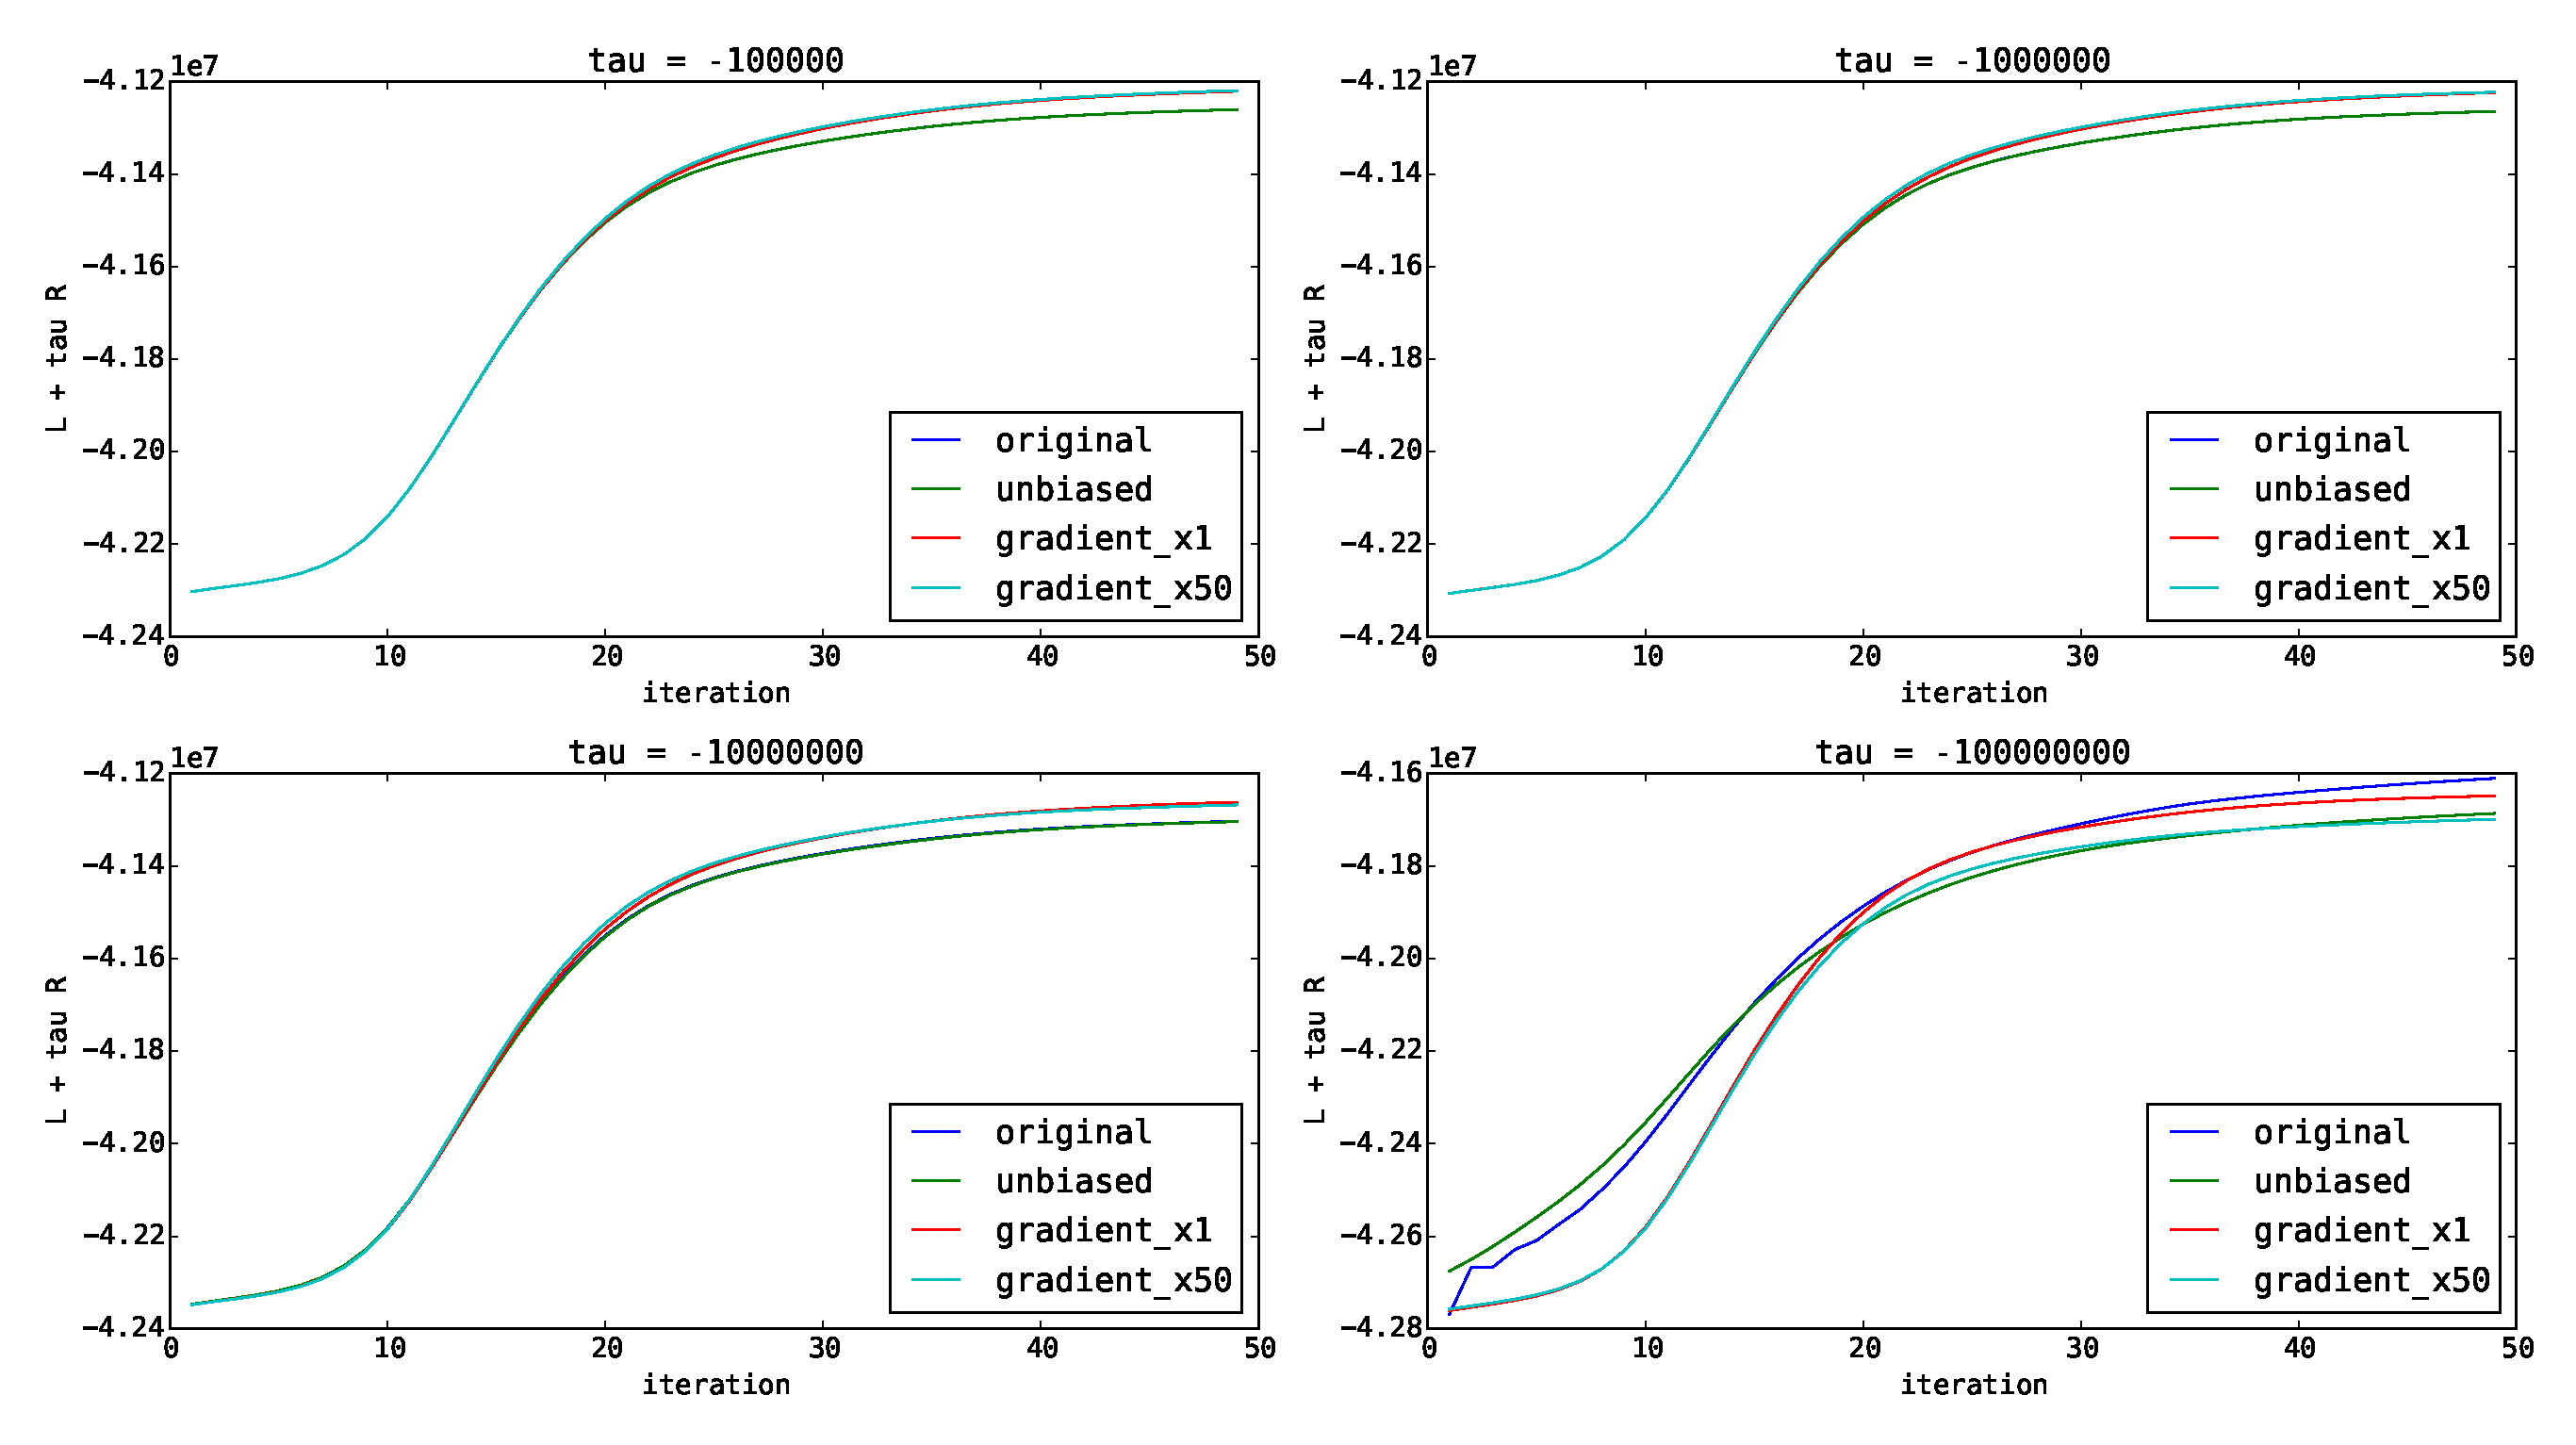
\includegraphics[width=1.0\linewidth]{pictures/topics_3_LR_values}
\end{figure}
\begin{figure}[H]
	\centering
	\caption{$|T| = 10$. Градиентные поправки немного хуже остальных, но при большом $|\tau|$ показывают ощутимо лучший результат.}      
	\medskip
	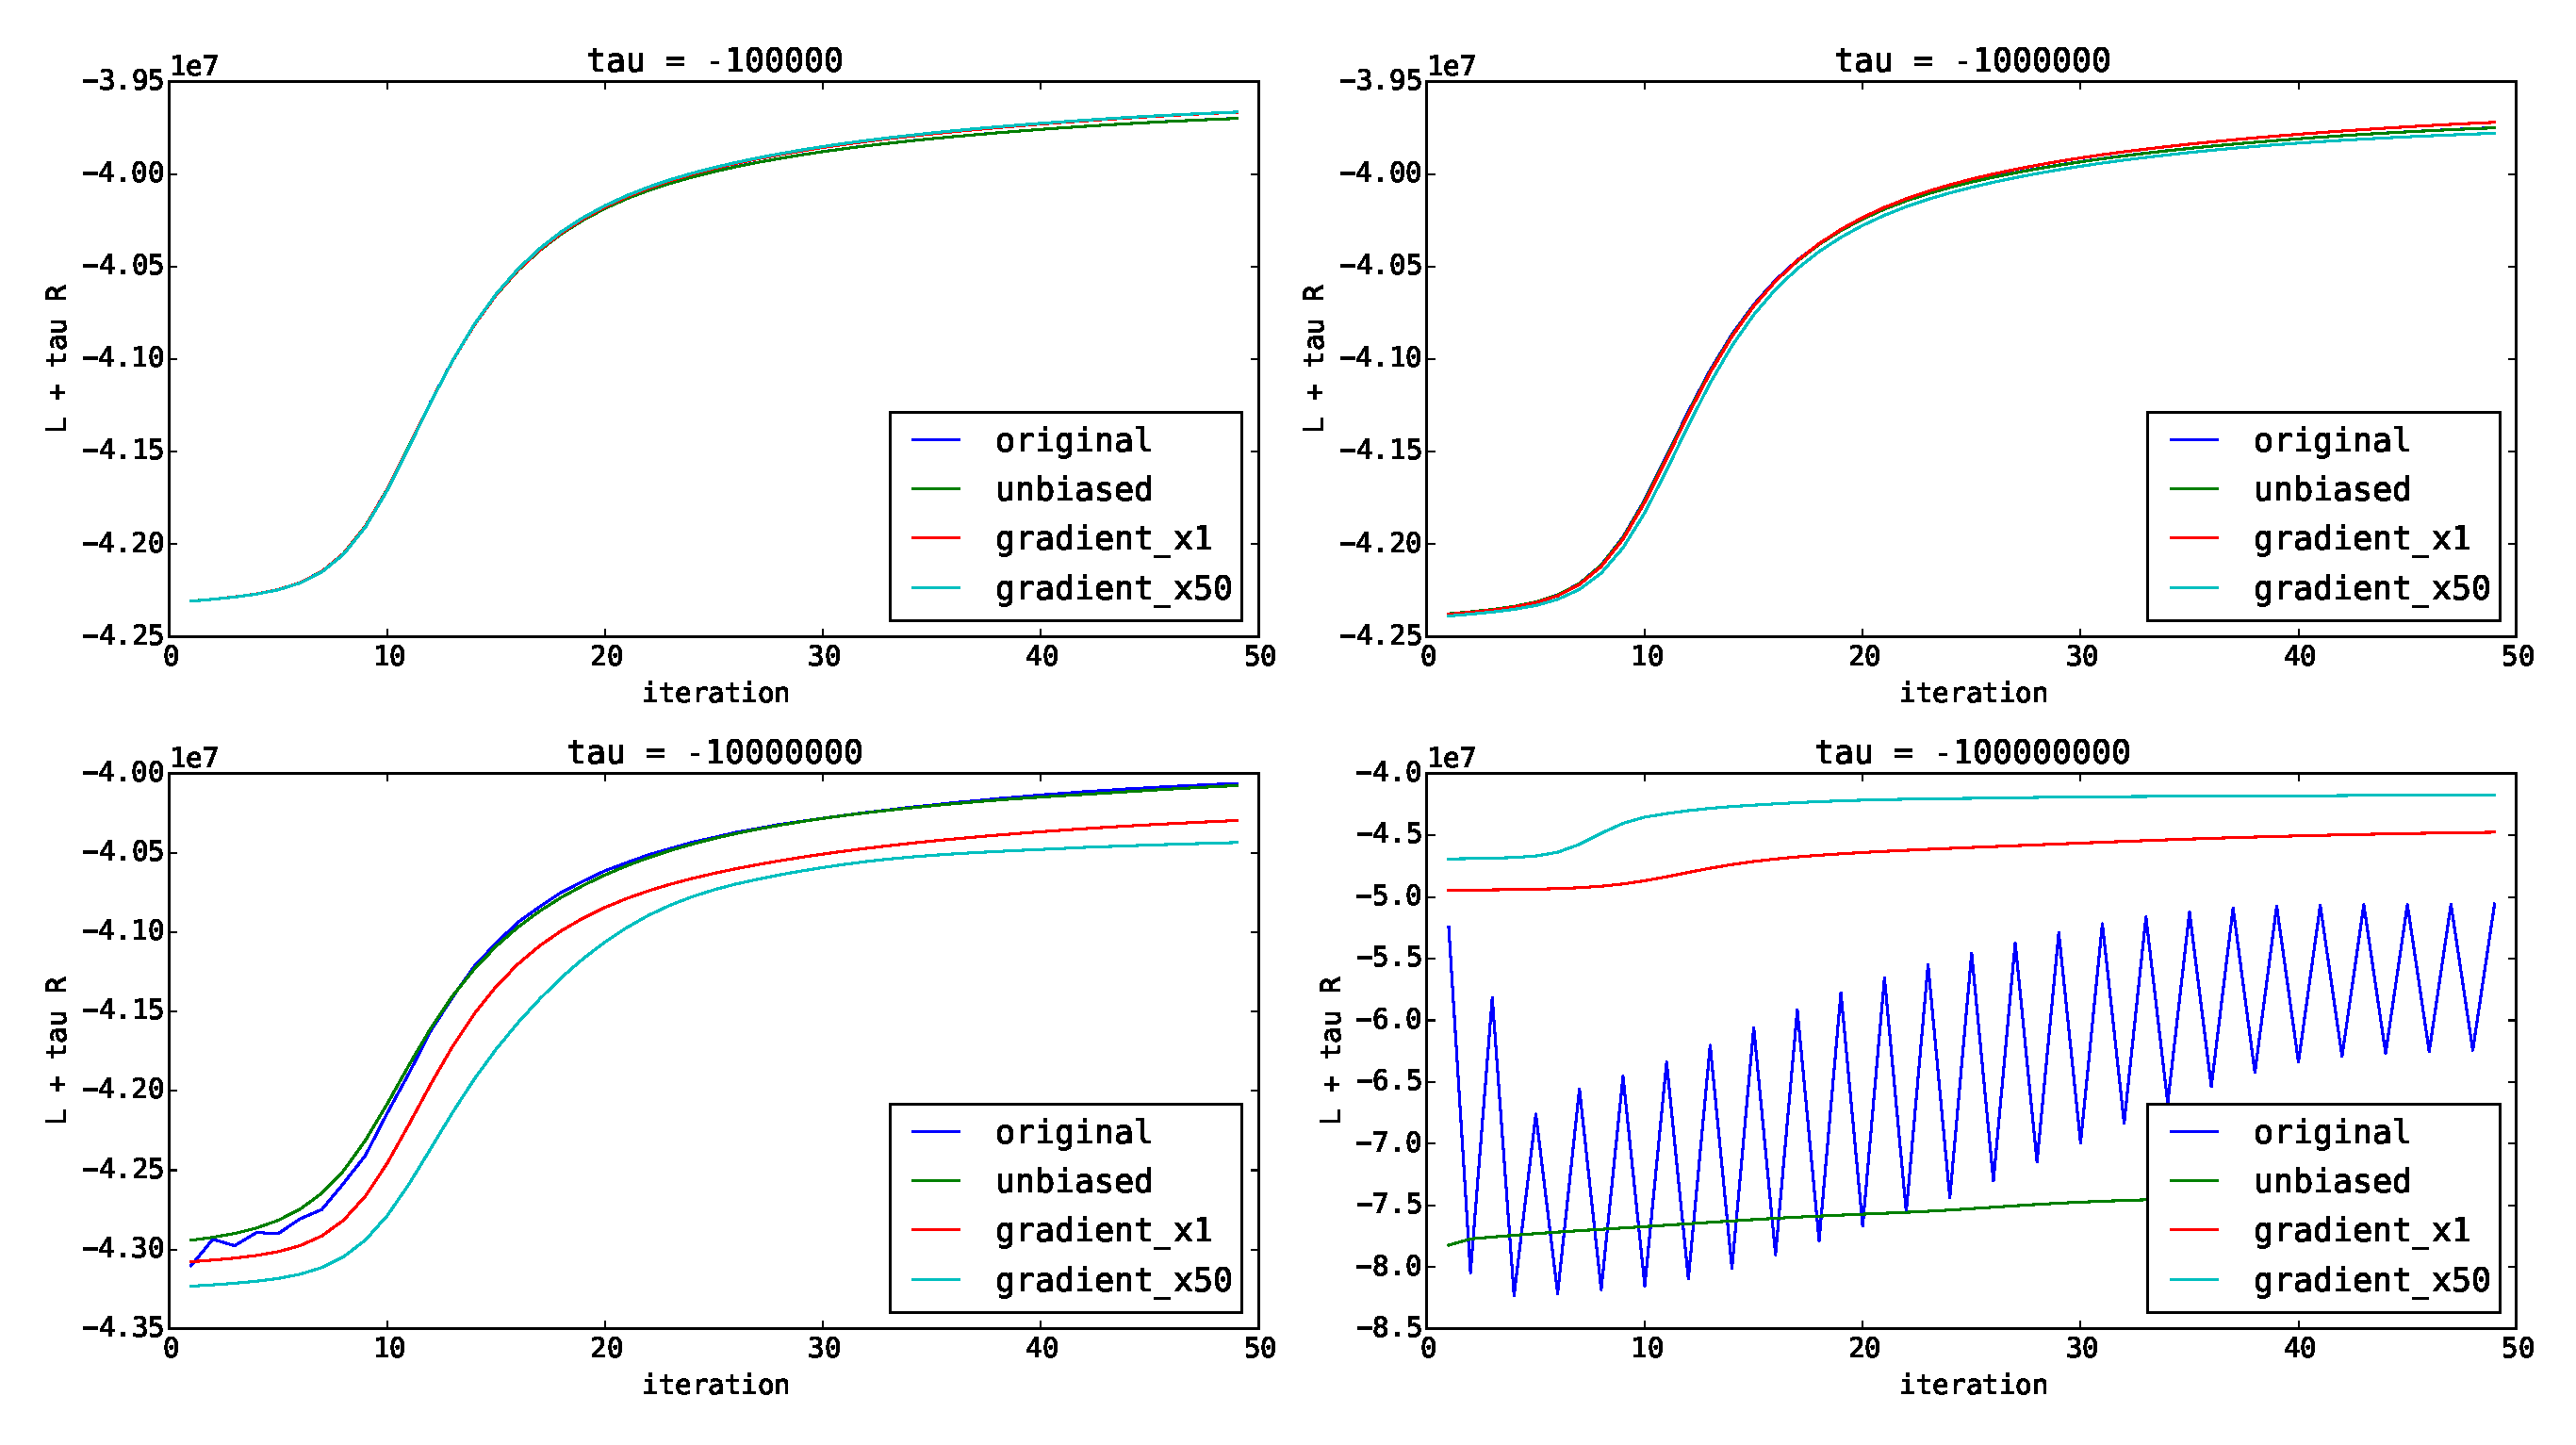
\includegraphics[width=1.0\linewidth]{pictures/topics_10_LR_values}
\end{figure}
\begin{figure}[H]
	\centering
	\caption{$|T| = 30$. Скачки начинаются при меньших $|\tau|$, до этого градиентные поправки так же немного хуже.}      
	\medskip
	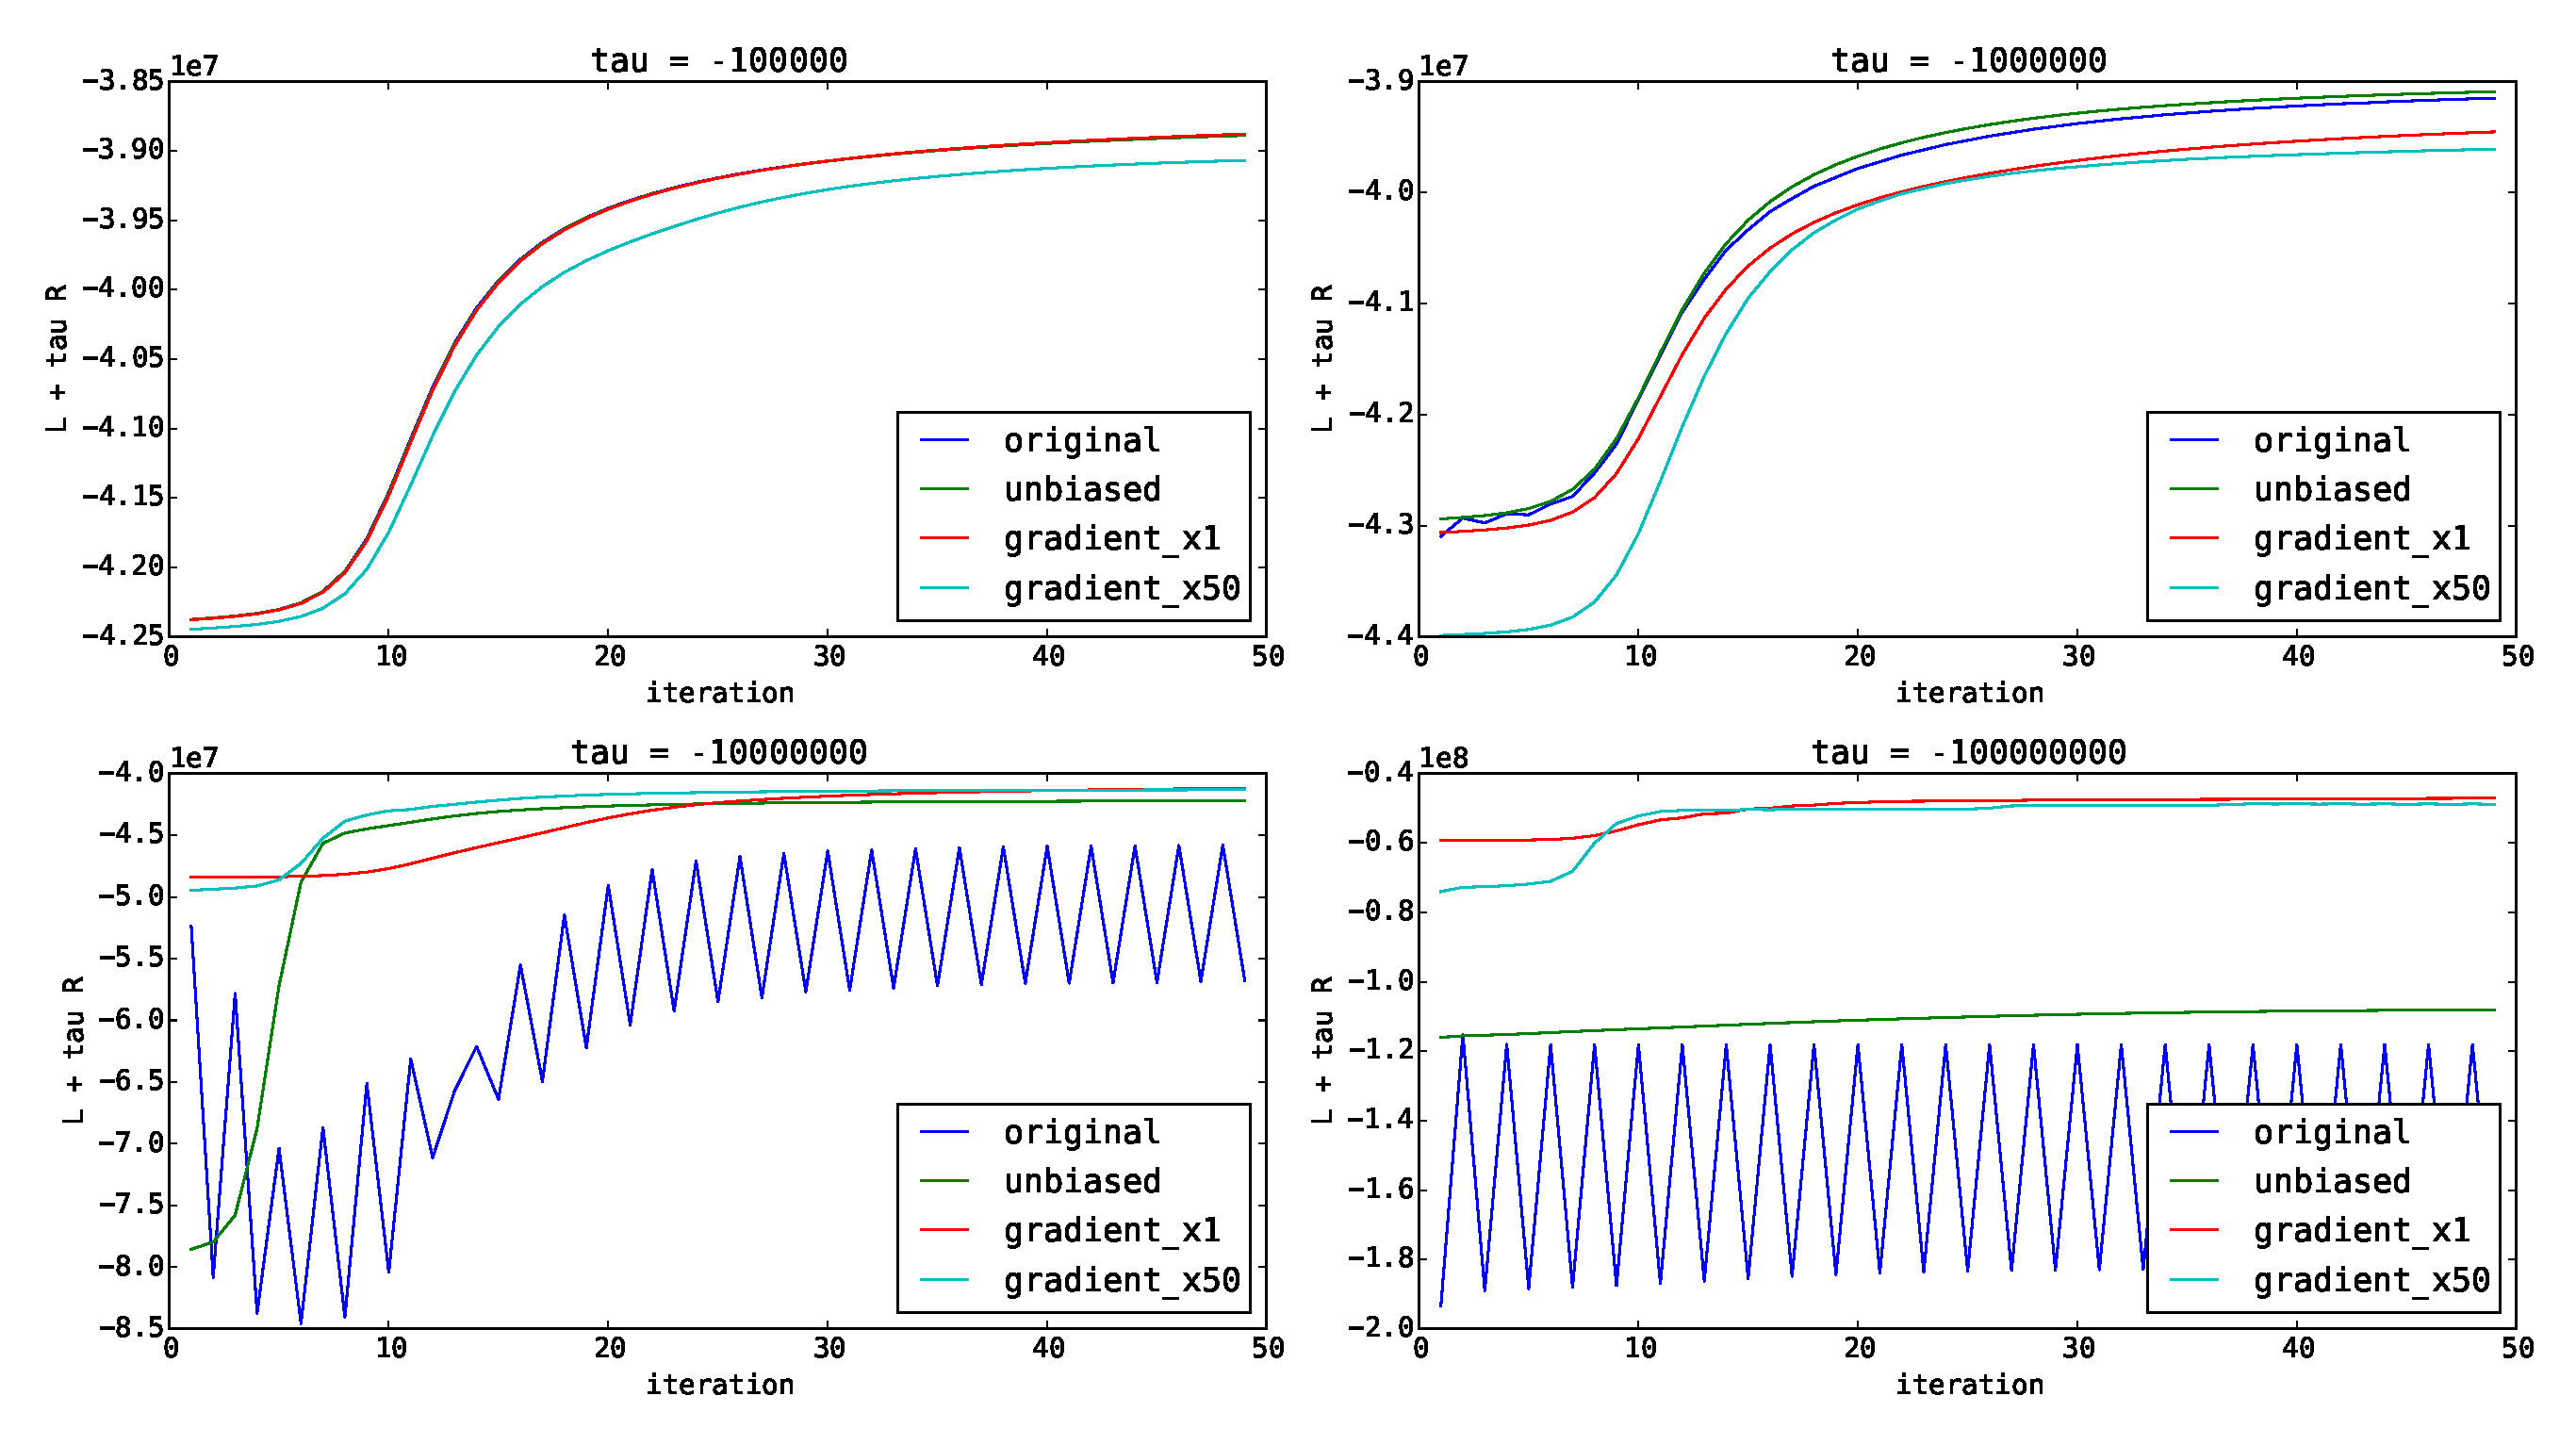
\includegraphics[width=1.0\linewidth]{pictures/topics_30_LR_values}
\end{figure}

Иногда градиентная поправка показывает чуть более слабые результаты. Это можно объяснить тем, что константы, на которые домножается градиент регуляризатора, выбраны не совсем удачно. Подбор данных констант это направление будущих исследований. 

Также стоит отметить, что  графики несмещённой модификации и стандартного М-шага практически не отличаются. Однако, с ростом $|\tau|$ можно увидеть, что начинаются скачки на графике стандартной формулы, а на графике несмещённой модификации их нет. Это связано с тем, как именно считаются регуляризационные поправки. Подробнее этот эффект будет обсуждён в следующей главе на графиках значений $R$, где он будет сильнее заметен.

Зависимость от числа тем  удобнее рассмотреть на значениях функционала $R$.

При очень большом значении $\tau$ графики для стандартной и несмещённой оценки резко падают. Этот эффект вызван следующим: стандартные формулы и несмещённая модификация зануляют слишком много параметров, что приводит к падению правдоподобия (нарушается свойство справедливости регуляризатора \ref{fairreg}), в то время как градиентная поправка, которая более аккуратно зануляет параметры, не создает провал логарифма правдоподобия.
\subsubsection{Значения $R$}
Регуляризатор $R$ и коэффициент $\tau$  вводились из соображений, что требуется найти такое решение задачи, в котором $\tau R \to \max$. Поскольку в рассматриваемом случае $\tau < 0$, то требуется $R \to \min$.\\
\begin{figure}[H]
	\centering
	\caption{$|T| = 3$. Значения $R$ очень малы по сравенению с $L$, поэтому при малых значениях $|\tau|$ оказывается, что оптимизировать $L$ существенно выгоднее чем $R$, и можно наблюдать немонотонную зависимость $R$ от итераций. Посколько значения $R$ практически не влияют на оптимизацию, то эффект скачков выражен неярко. Градиентные поправки заметно хуже оптимизируют $R$.}    
	\medskip
	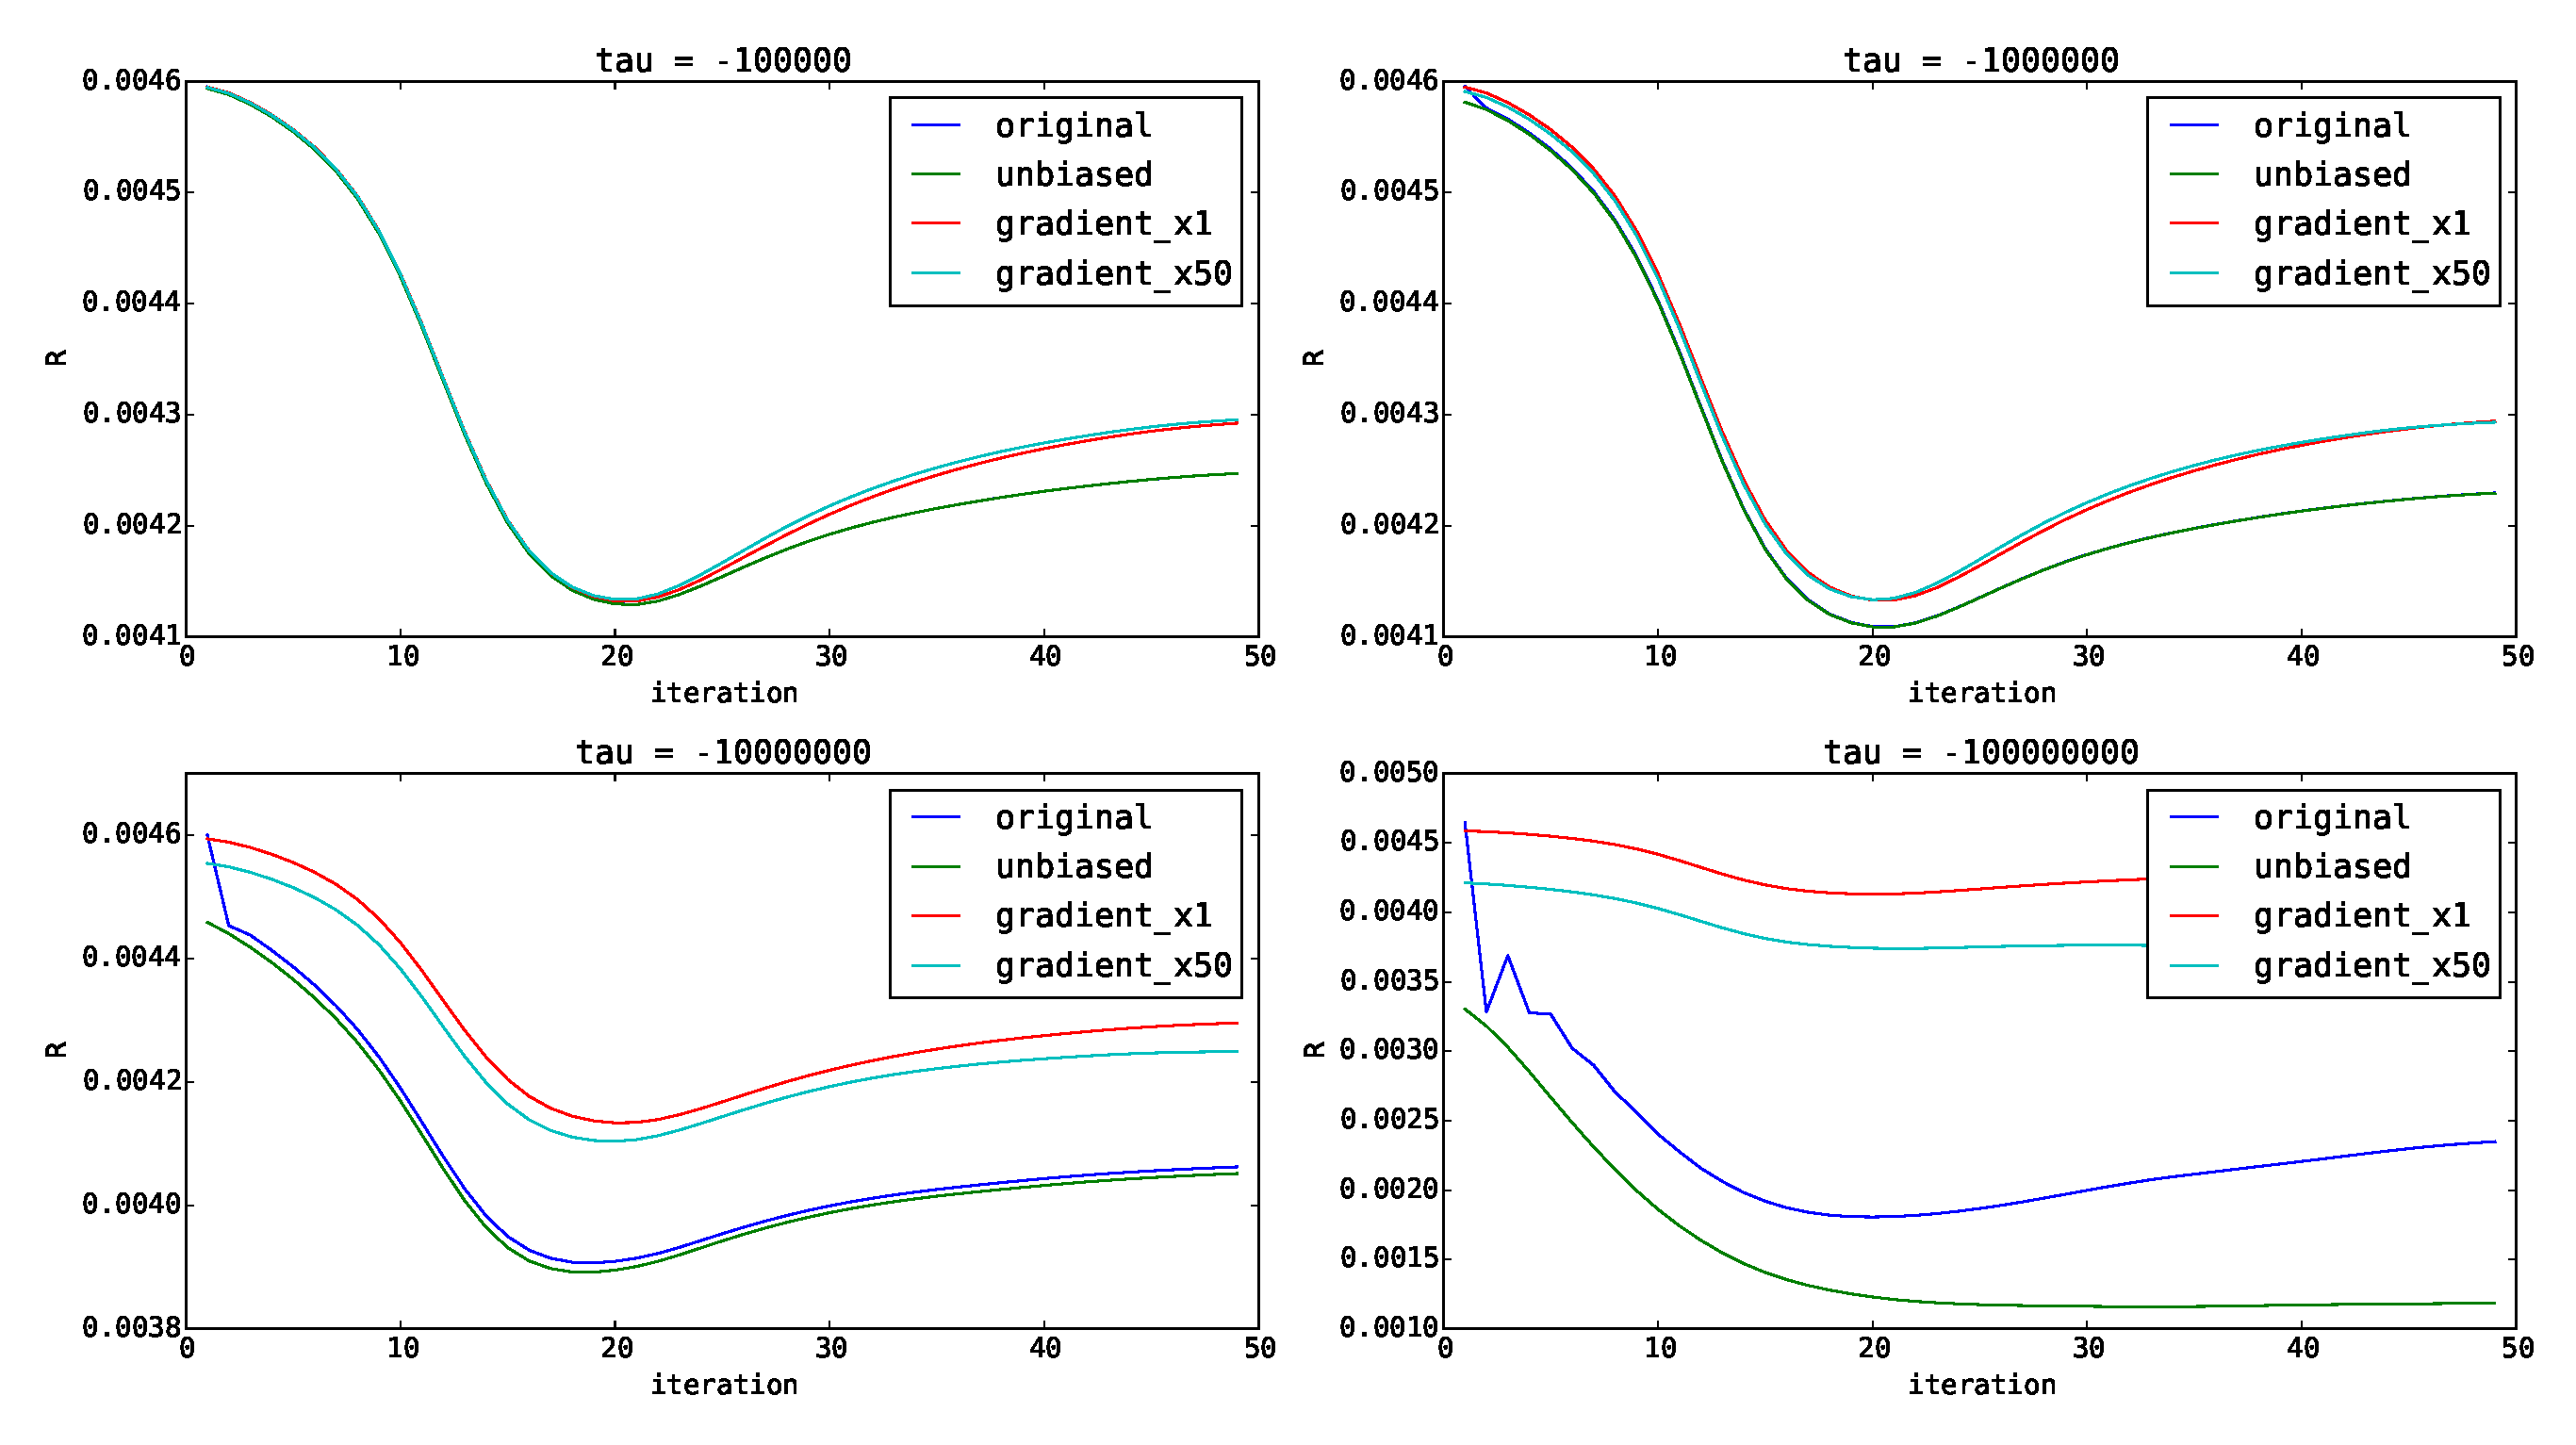
\includegraphics[width=1.0\linewidth]{pictures/topics_3_R_values}
\end{figure}
\begin{figure}[H]
	\centering
	\caption{$|T| = 10$. На верхних графиках виден скачок $R$ на первой итераций, на нижних графиках он ярче выражен. Несмещённая модификация и градиент $\times 50$  лучше всех остальных.}    
	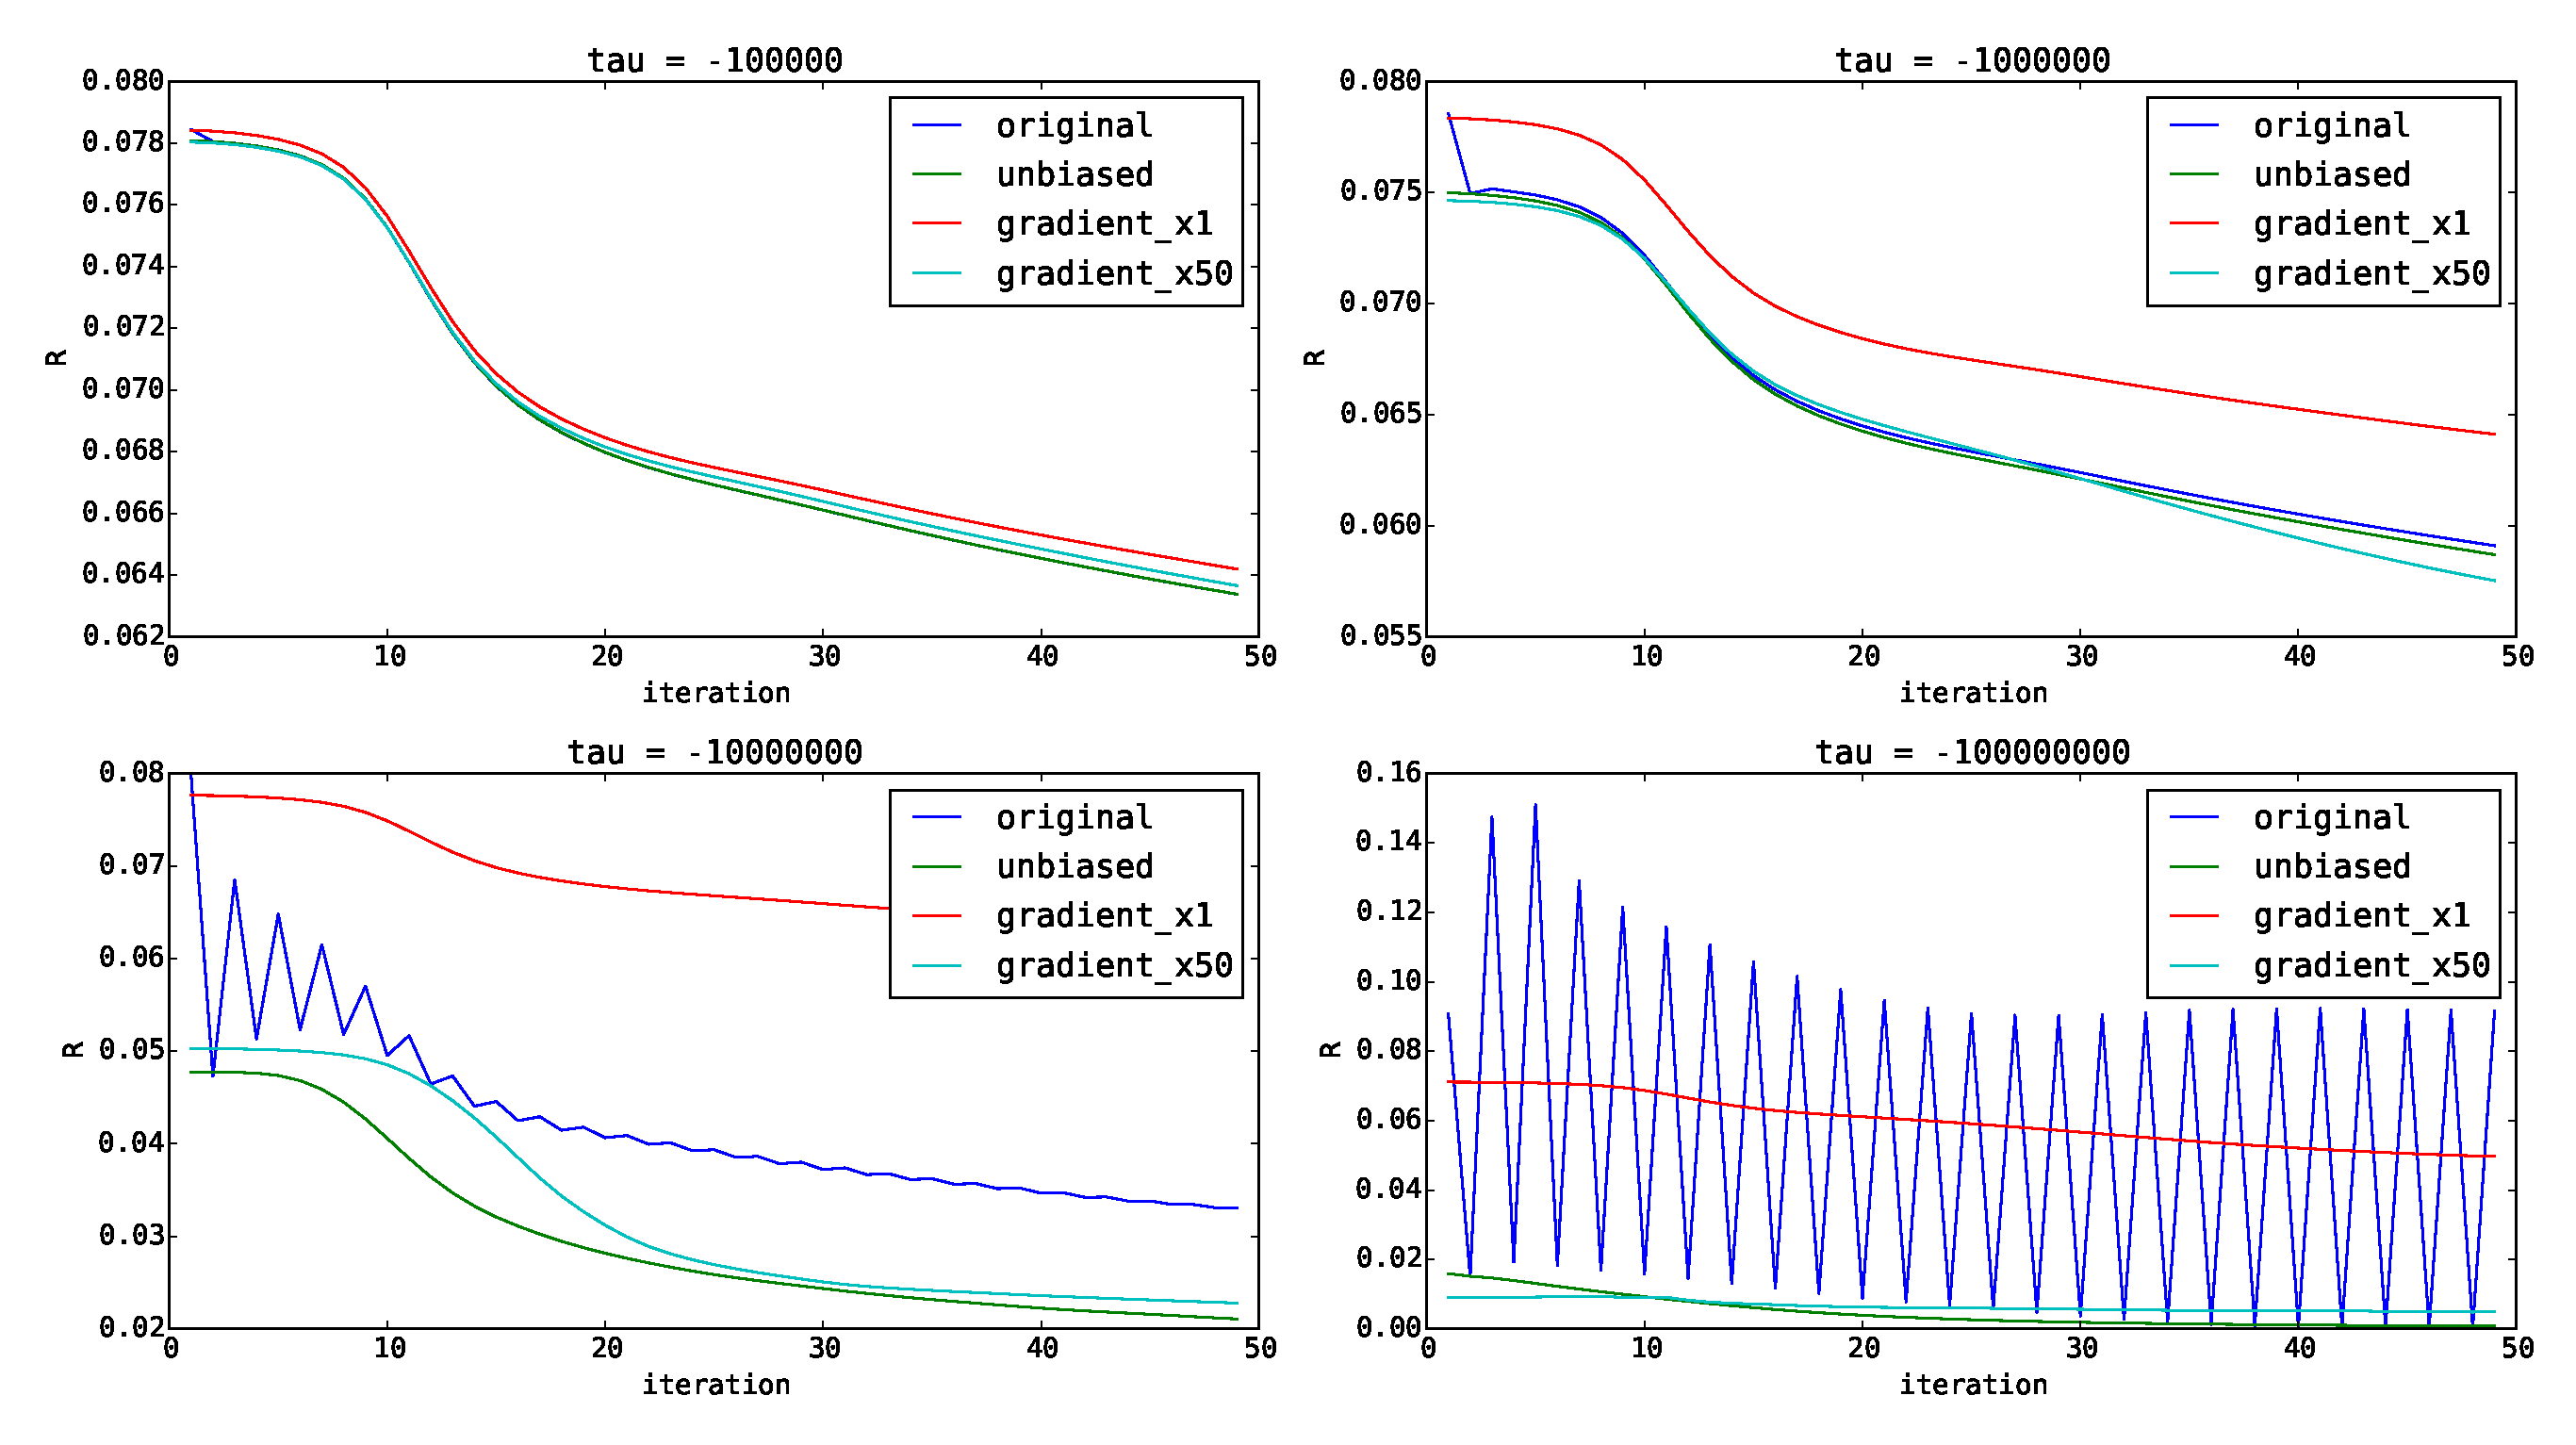
\includegraphics[width=1.0\linewidth]{pictures/topics_10_R_values}
\end{figure}
\begin{figure}[H]
	\centering
	\caption{$|T| = 30$. Эффект скачков уже ярко выражен при $\tau = -10^6$. Градиент $\times 50$ существенно лучше всех остальных.}    
	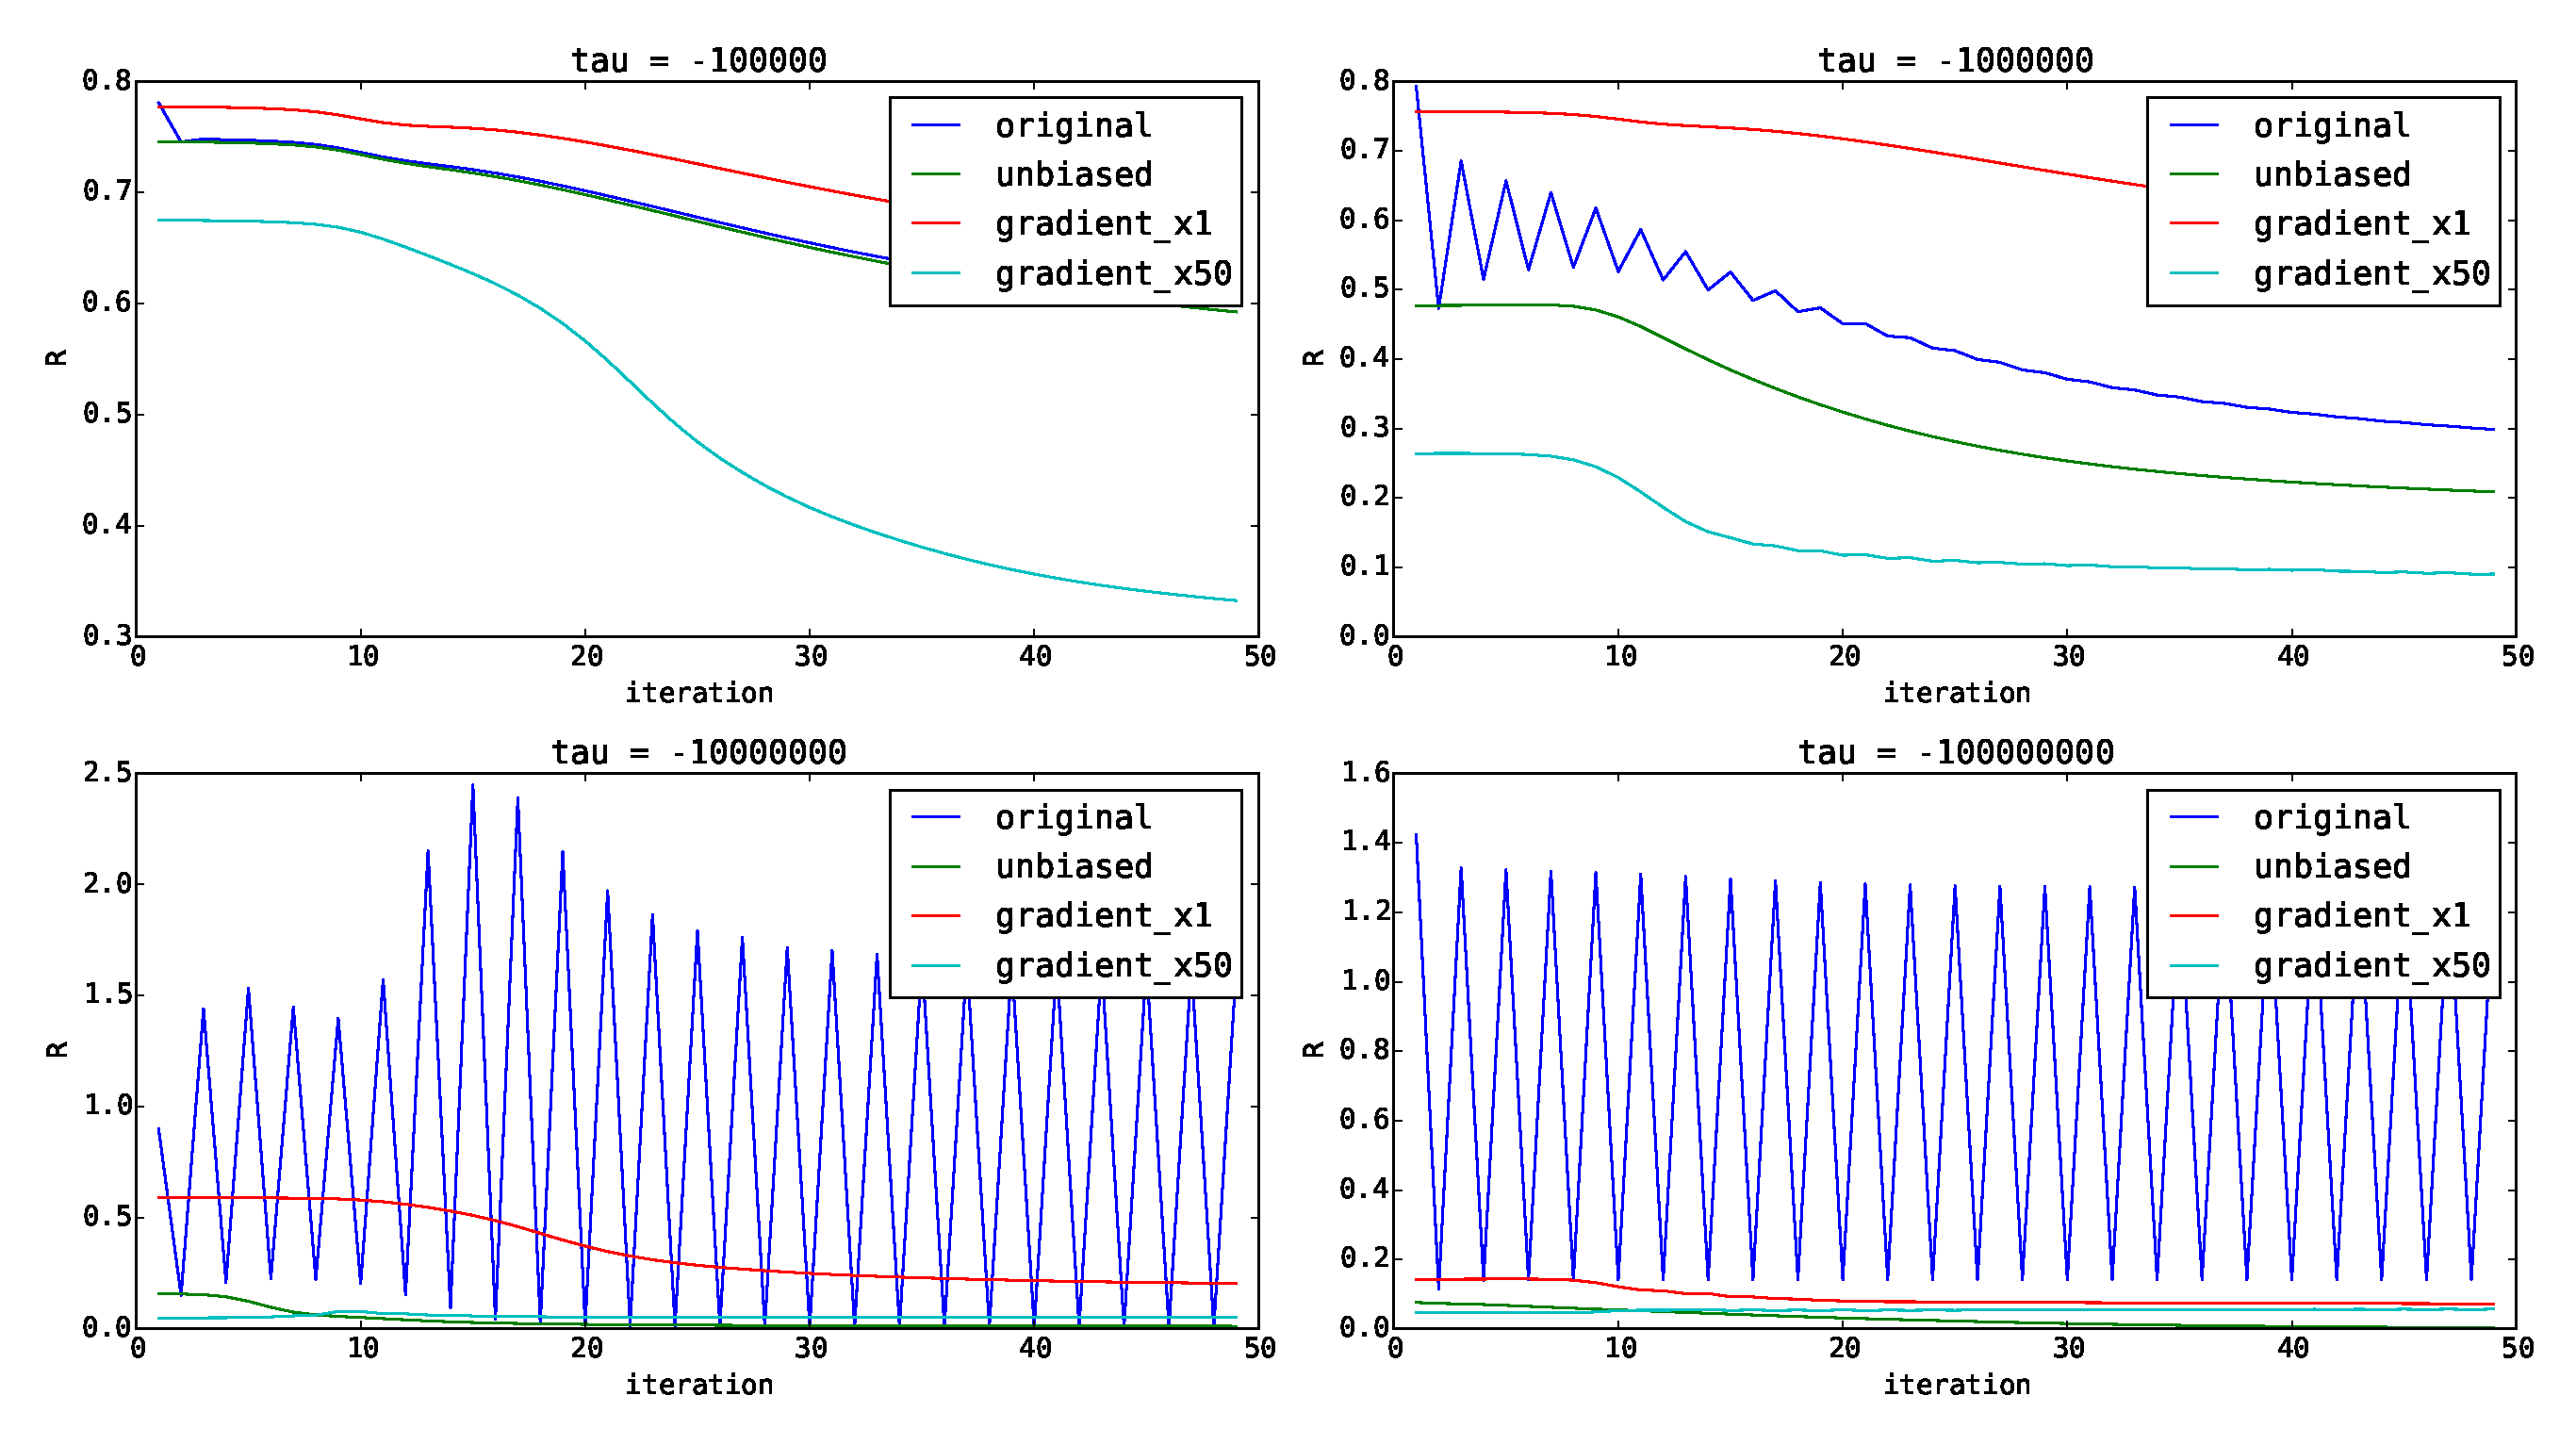
\includegraphics[width=1.0\linewidth]{pictures/topics_30_R_values}
\end{figure}

При достаточно больших значения $|\tau|$ видно, что в стандартной  формуле М-шага есть скачки в изменении $R$ на первых итерациях. Это вызвано тем, что регуляризационные поправки считаются в точке с предыдущей итерации. На первых итерациях  она слабо связана с точкой $\left( \frac{n_{wt}}{{n_t}}, \frac{n_{td}}{n_d}\right)$, к которой применяется регуляризационное преобразование. Конечно, со временем $(\phi_{wt}, \theta_{td})$ стремятся к $\left( \frac{n_{wt}}{{n_t}}, \frac{n_{td}}{n_d}\right)$. Это можно видеть на графиках --- они постепенно спрямляются. Но на первых итерациях $(\phi_{wt}, \theta_{td})$ существенно отличается  от $\left( \frac{n_{wt}}{{n_t}}, \frac{n_{td}}{n_d}\right)$  и эффект скачков  проявляется, а большое значение $|\tau|$ усиливает различие и делает эффект более ярким.

С ростом числа тем порядок значений $R$ изменился, и поэтому чувствительность к $|\tau|$ возросла. Как следствие, можно наблюдать, что колебания значений функционала начинаются раньше, размер этих колебаний существеннее, а градиентные поправки раньше начинают показывать лучшее качество, чем остальные алгоритмы.

Также стоит отметить интересный эффект при $|T| = 3$. Значения $R$ очень малы, и в итоге оптимизация $L$ выходит на первый план, что приводит к немонотонной траектории $R$. С ростом $\tau$ эта зависимость постепенно выпрямляется. Это хорошо иллюстрирует, как коэффициент регуляризации влияет на модель, увеличивая важность регуляризатора.
\subsubsection{Изменения $R$ на втором этапе М-шага}
Предложенные формулы выводились из соображений увеличения функционала $R$ при регуляризационном преобразовании. Чтобы проверить, правильность выведенных формул предлагается измерить изменение $R$ на данном этапе М-шага. Поскольку для выбранного регуляризатора стоит задача минимизации $R$, то чем меньше изменение, тем лучше. Также стоит отметить, что эффект скачков на первых итерациях будет здесь наиболее заметен, так как проявляется именно в данной величине, а все предыдущие замеры, совмещали данный эффект с другими.
\begin{figure}[H]
	\centering
	\caption{$|T| = 10$. Для несмещённой и стандартной формулы изменение существенно лучше, что подтверждает слова о неправильном выборе констант перед градиентом.}    
	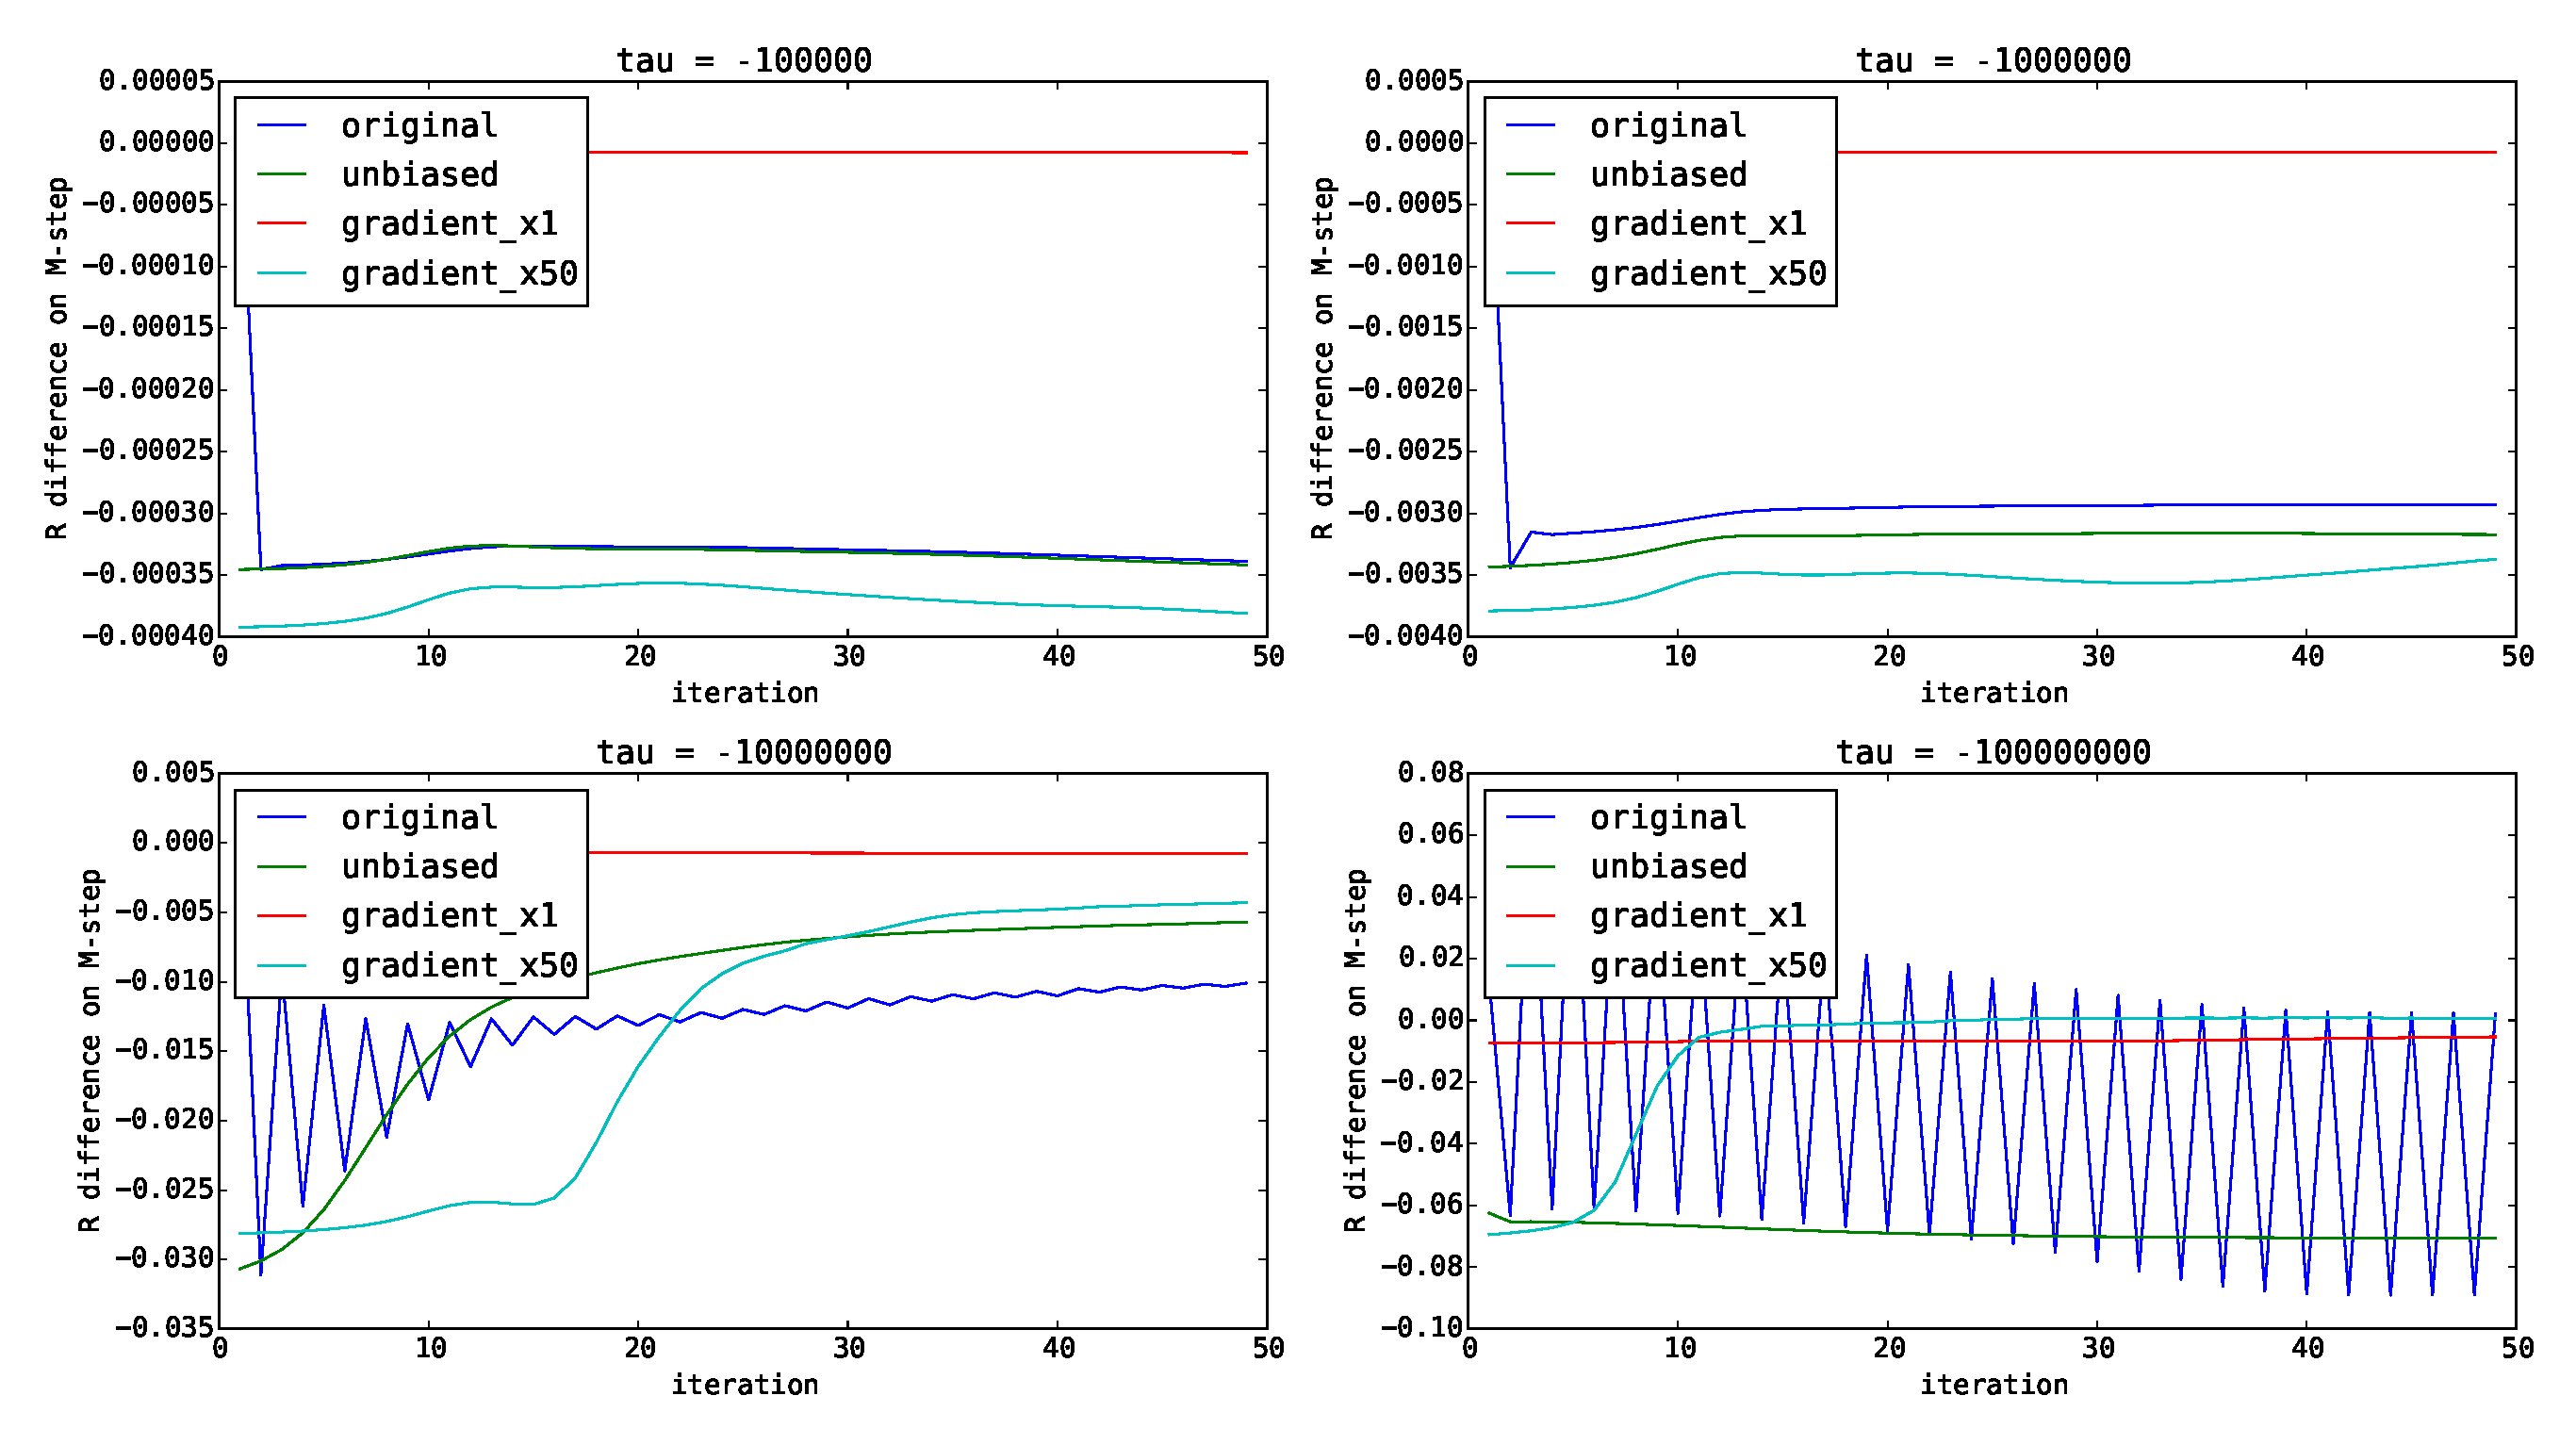
\includegraphics[width=1.0\linewidth]{pictures/topics_10_RMstepDiff}
\end{figure}

Другие графики аналогичны, поэтому не будут приведены. Чтобы сравнить формулы по изменению $R$ при регуляризационном преобразовании, предложено оценить удельный эффект (нормировать изменение на $l_1$ и $l_2$ нормы). Графики весьма однотипны, поэтому приведём только случай $|T| = 10$.

\begin{figure}[H]
	\centering
	\caption{$|T| = 10$. Стандартная формула и несмещённая модификация лучше по $l_1$ норме, градиентные поправки по $l_2$ норме. Эффект скачков хорошо выражен.}    
	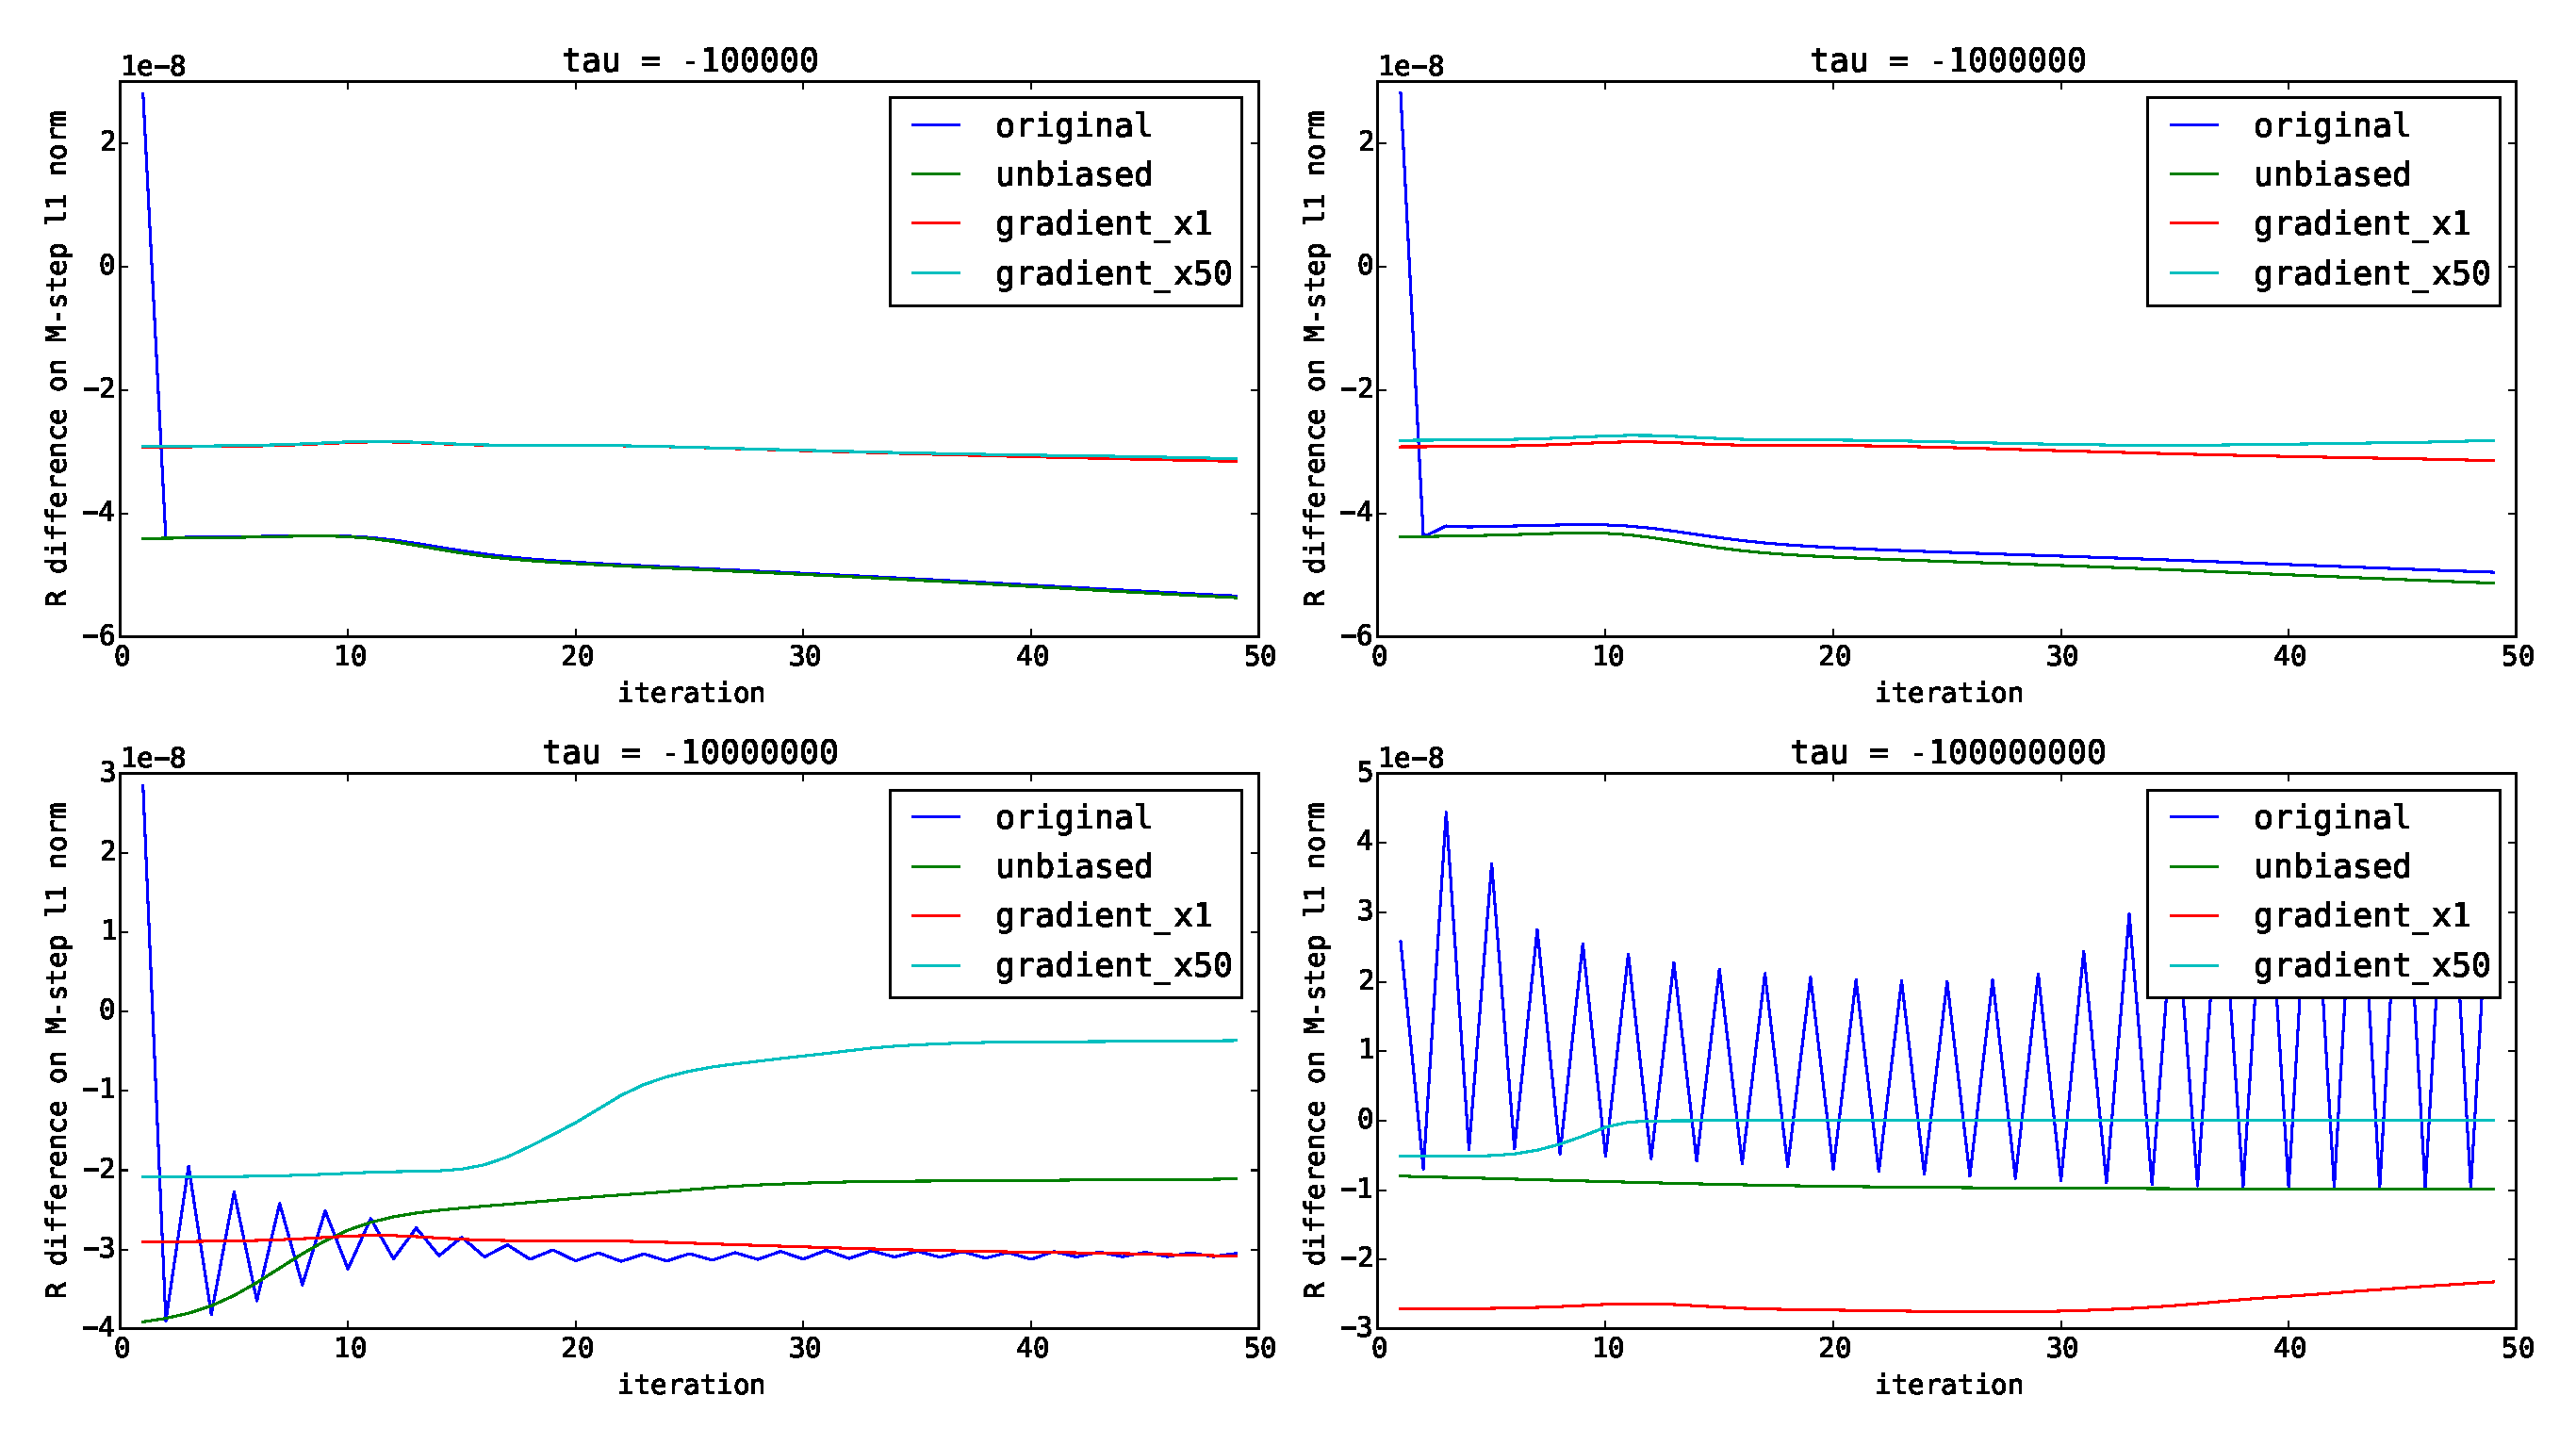
\includegraphics[width=1.0\linewidth]{pictures/topics_10_RMstepDiffPerL1}
	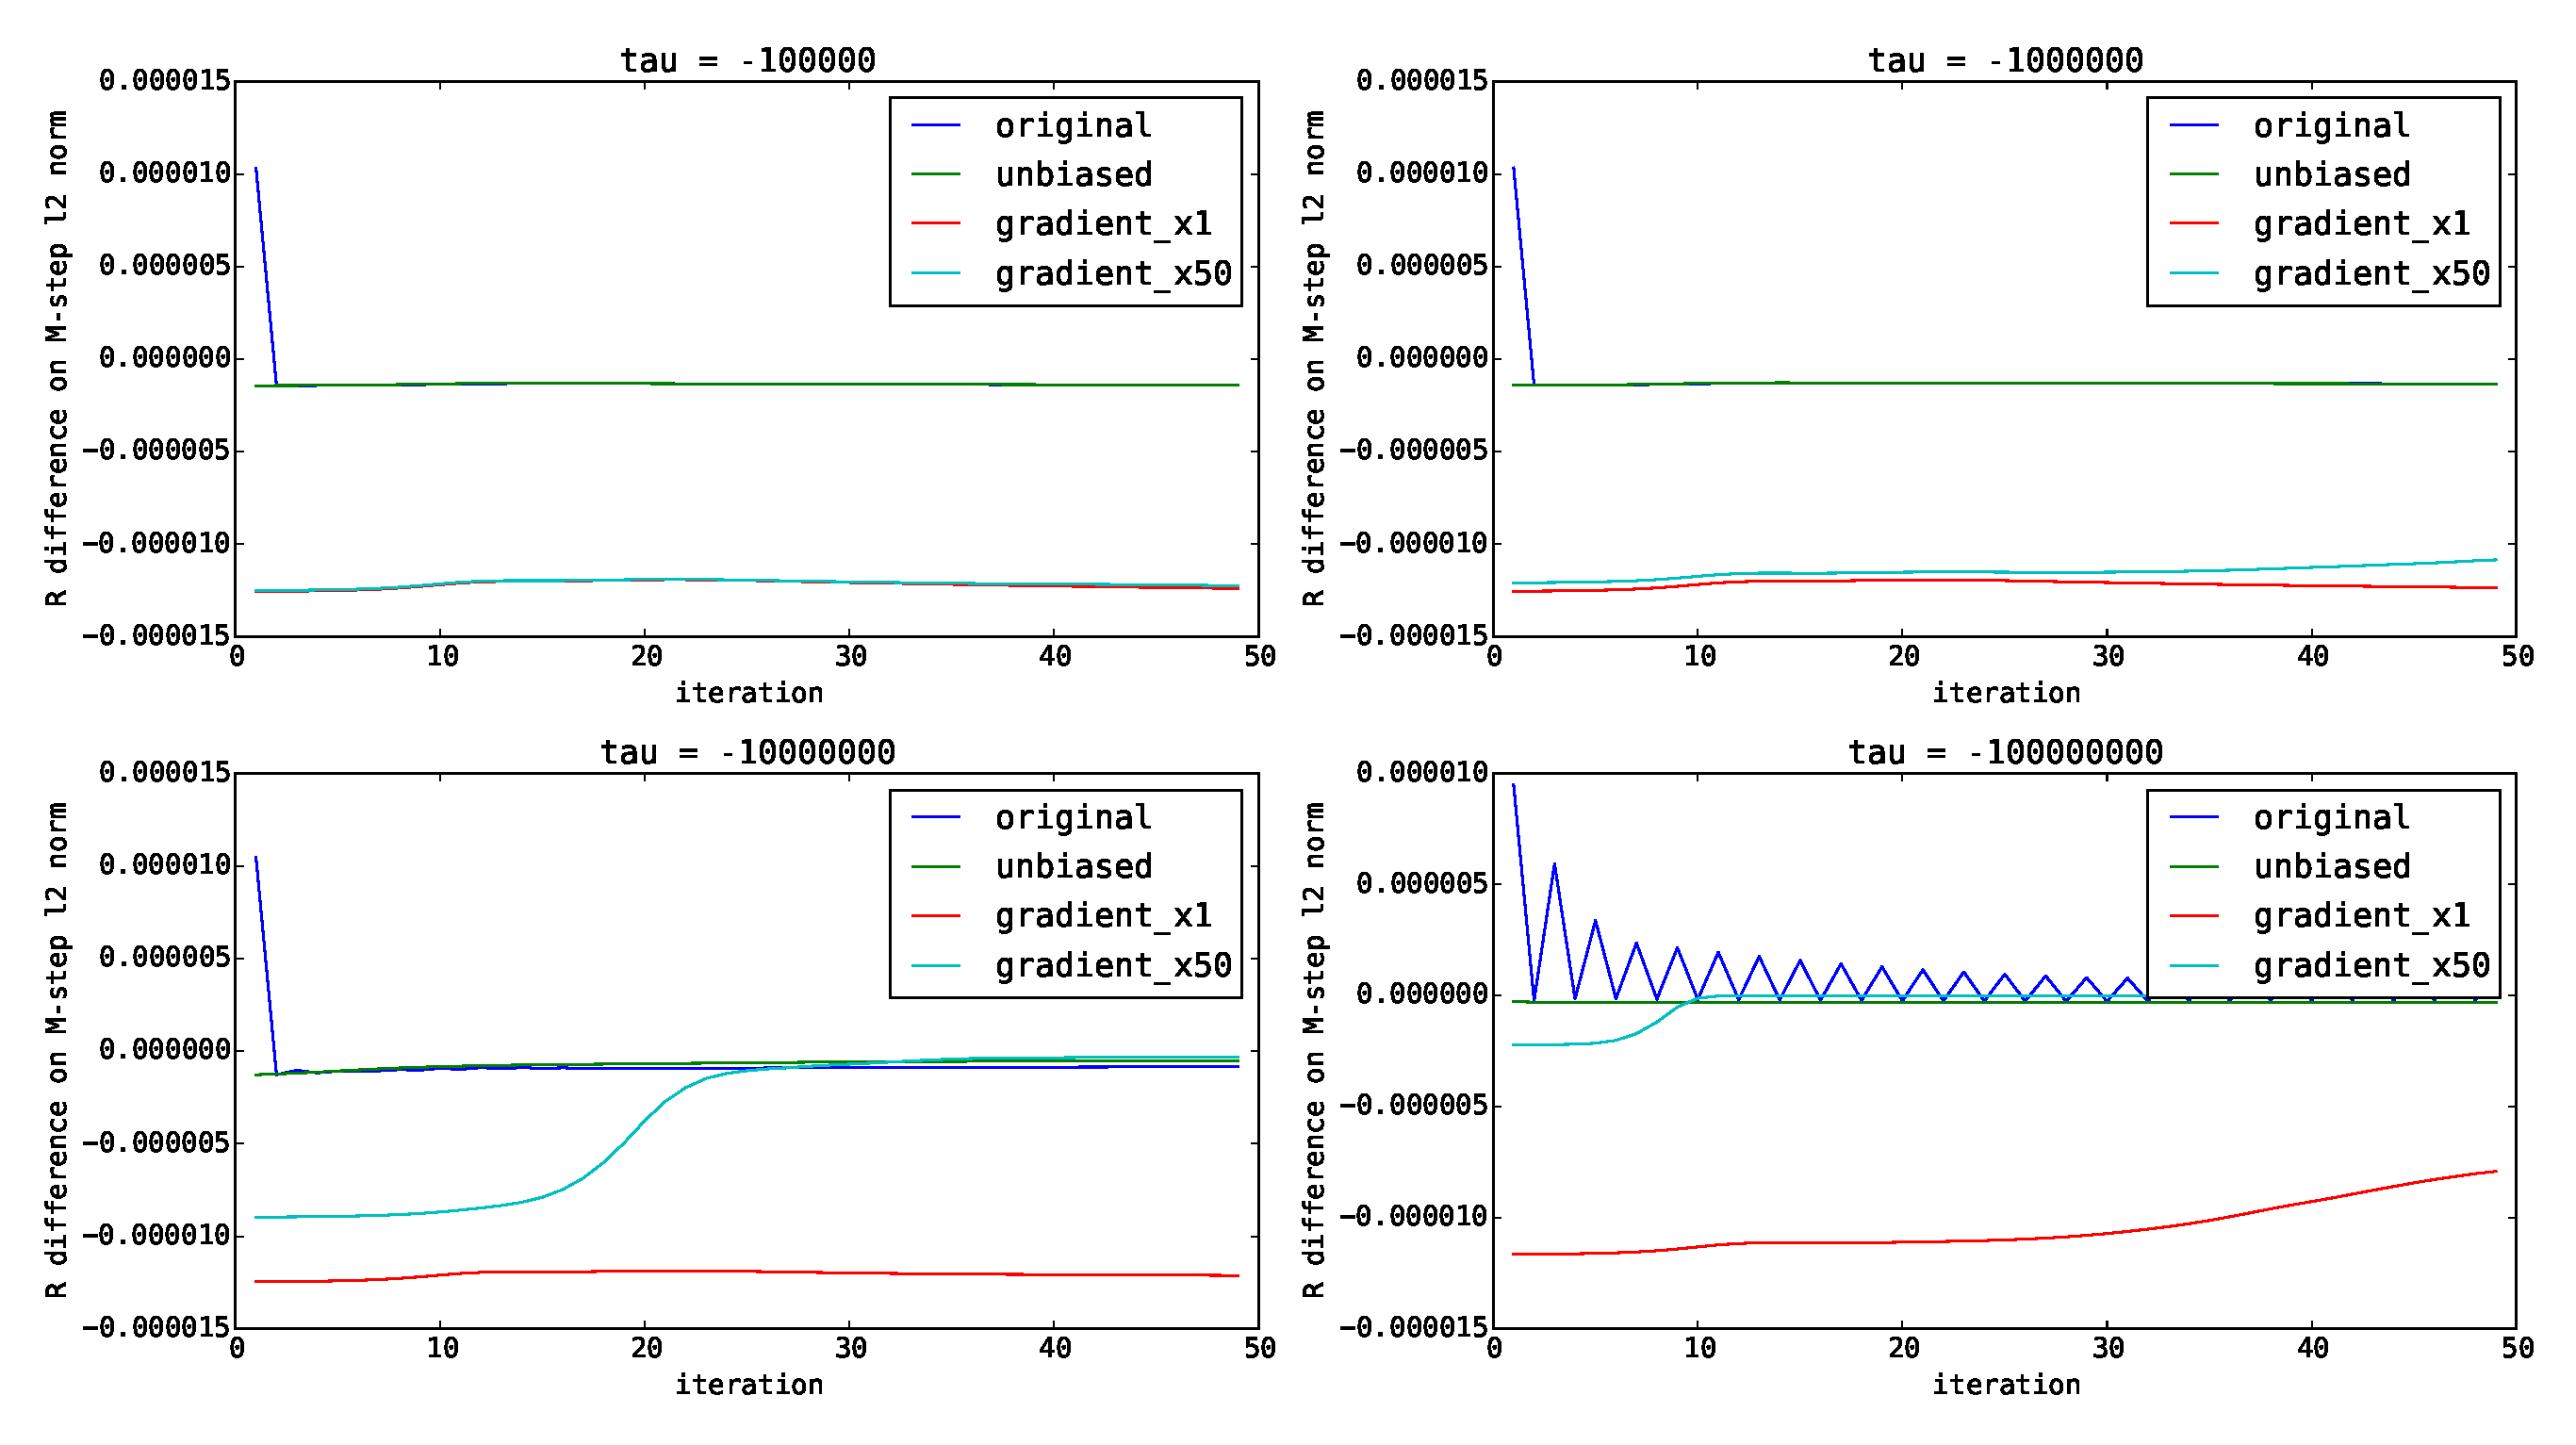
\includegraphics[width=1.0\linewidth]{pictures/topics_10_RMstepDiffPerL2}
\end{figure}

Для всех предложенных модификаций уменьшение значения $R$ на втором этапе М-шага заметно больше, чем в стандартном алгоритме, что ожидаемо, поскольку они были выведены с такой целью. Поскольку градиент --- это оптимальное направление изменения в $l_2$ норме, то при нормировке изменения $R$ на $l_2$ норму получаем, что градиентные поправки существенно эффективнее двух других методов.

С ростом $|\tau|$ можно наблюдать эффект насыщения, то есть эффективность поправок падает с итерациями, что означает приближение к стационарной точке $R$, это положительно говорит о предложенных модификациях.
\subsubsection{Минимальное значения в $\Phi$ и $\Theta$}
Важным свойством при доказательстве сходимости была $\varepsilon$-разреживаемость регуляризатора, поэтому требуется проверить данное предположение. На графиках изображены логарифмы минимальных ненулевых значений в матрицах $\Phi$ и $\Theta$.
\begin{figure}[H]
	\centering
	\caption{$|T| = 3$. Для матрицы $\Phi$ градиентные поправки имеют большую отделимость от нуля. На матрице $\Theta$ различия несуществены при отсутсвии эффекта скачков и сверхбольшого $|\tau|$.}    
	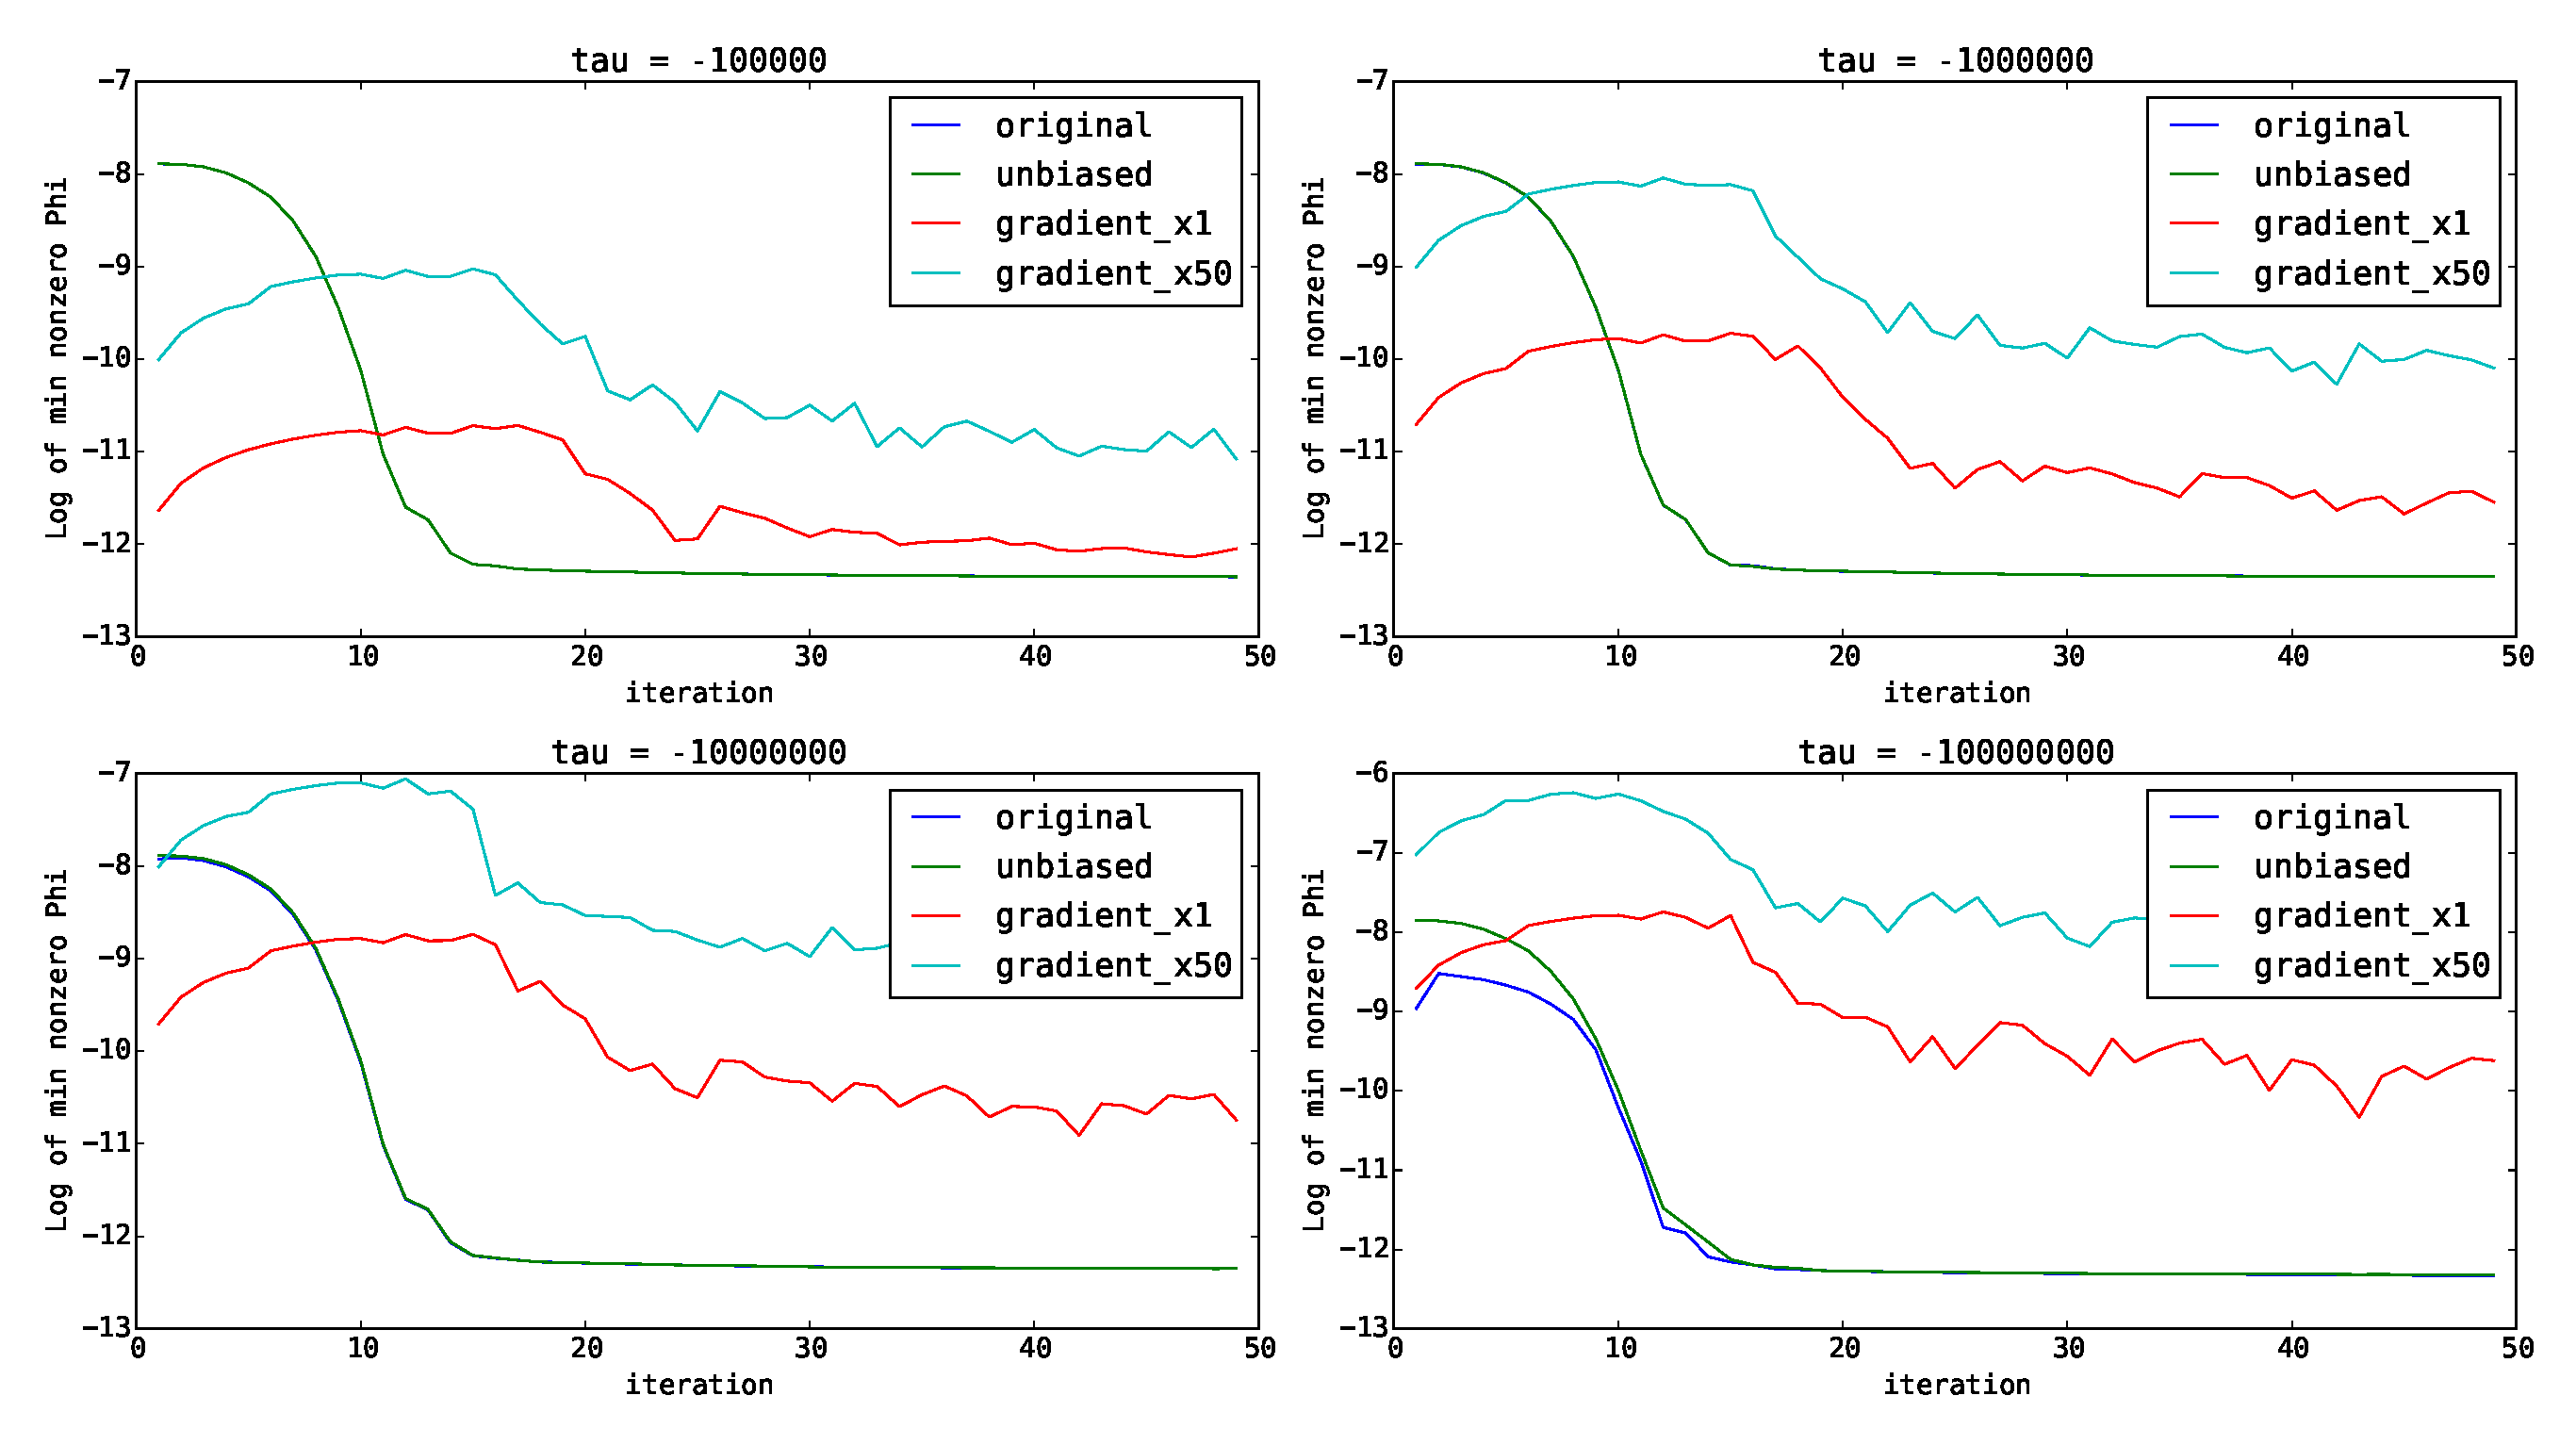
\includegraphics[width=1.0\linewidth]{pictures/topics_3_minPhi_values}
	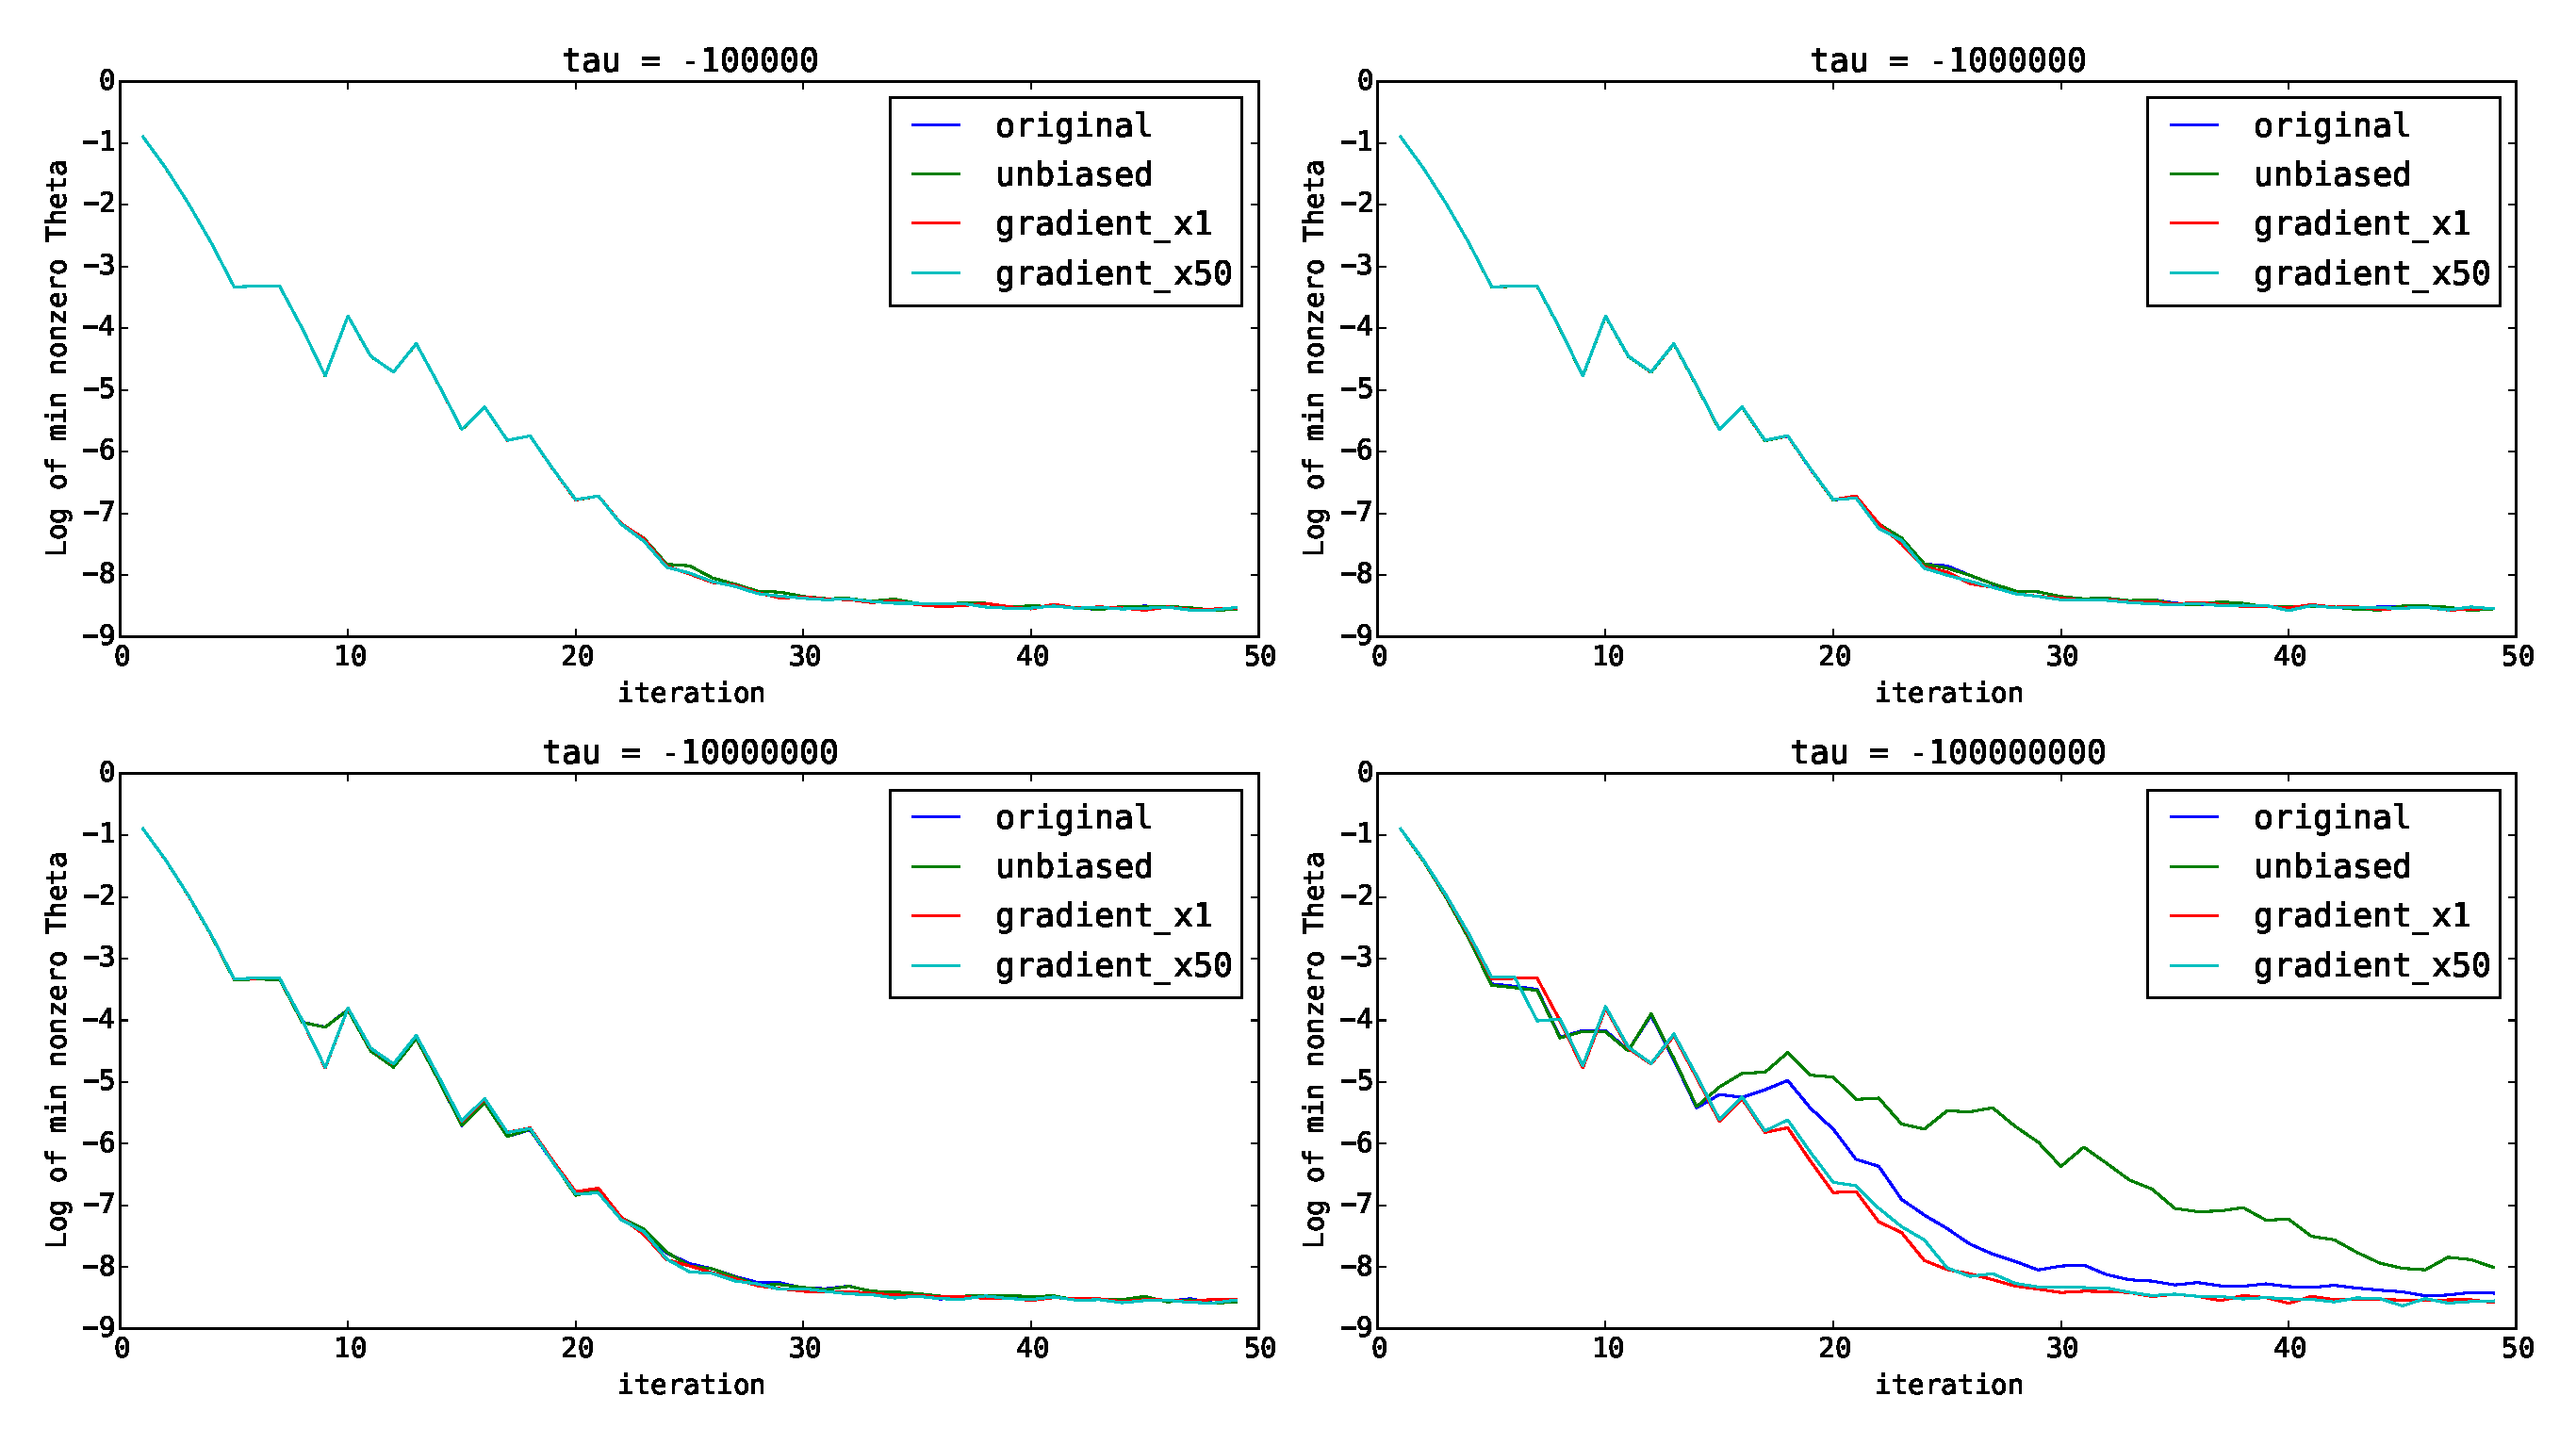
\includegraphics[width=1.0\linewidth]{pictures/topics_3_minTheta_values}
\end{figure}
\begin{figure}[H]
	\centering
	\caption{$|T| = 10$. Графики несмещённой модификации и стандартной формулы стабилизируются на некотором значении, это вызвано технической особенностью, описанной в главе \ref{technical}.}    
	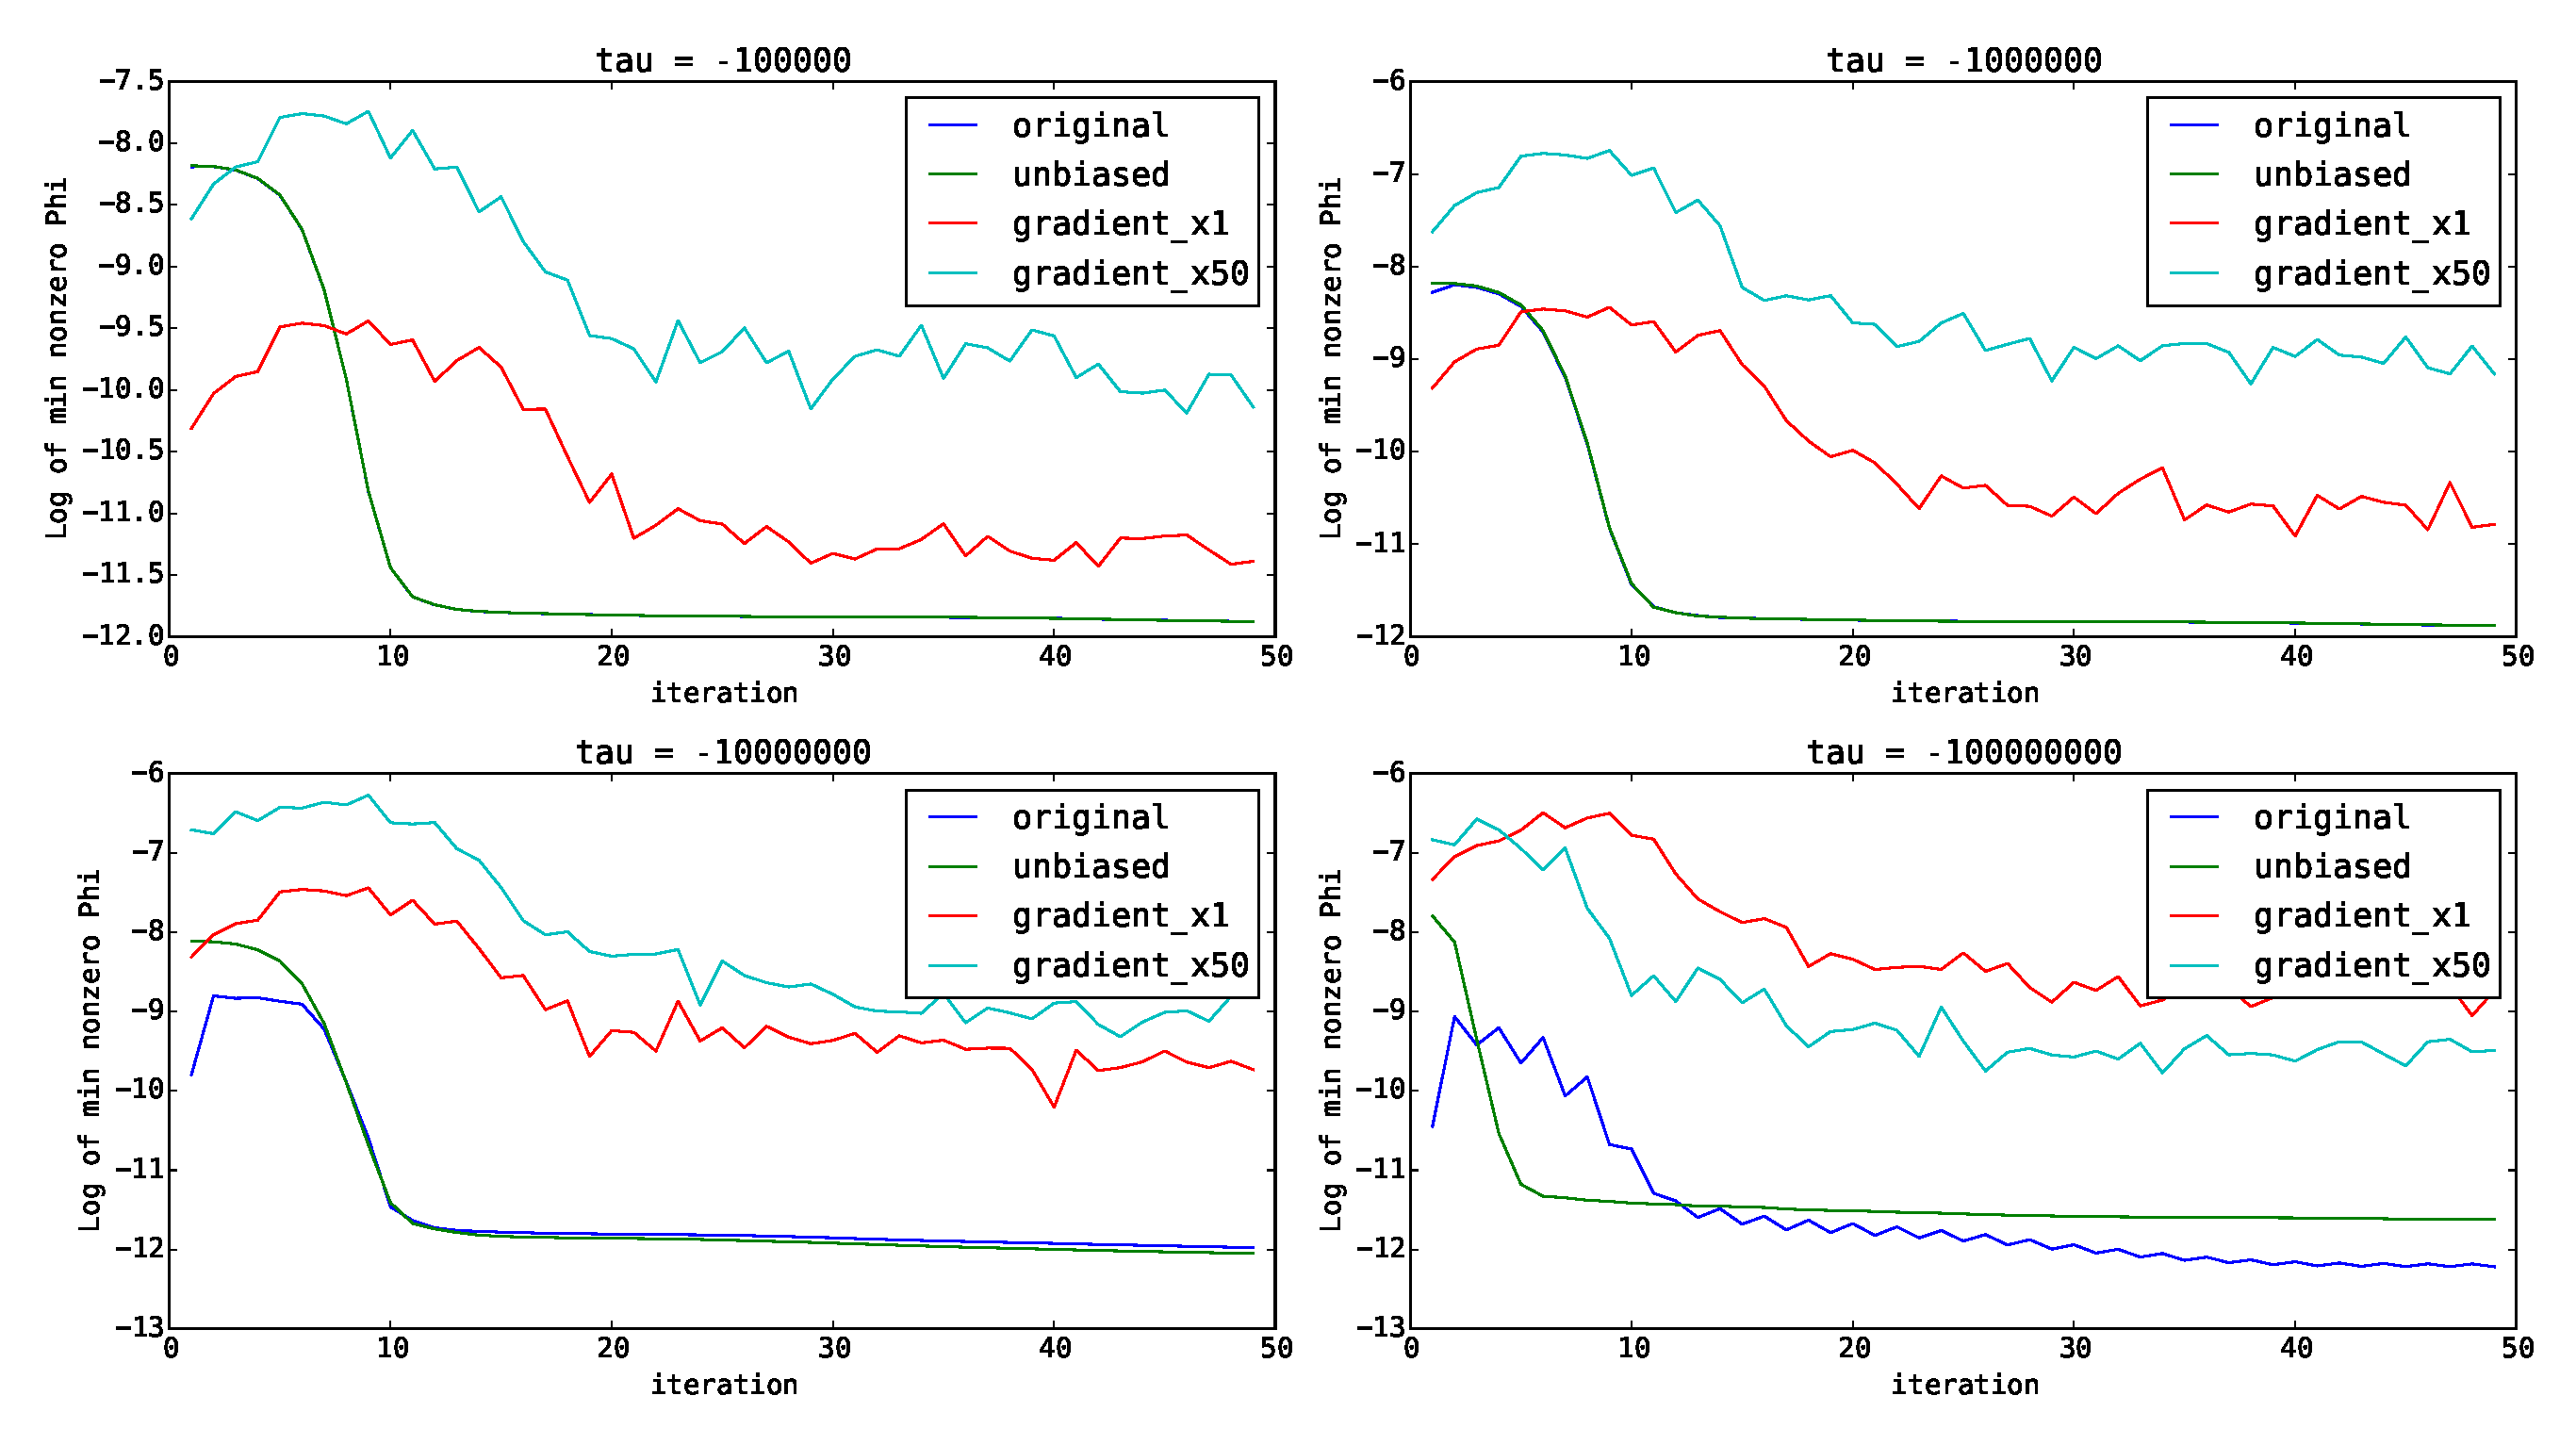
\includegraphics[width=1.0\linewidth]{pictures/topics_10_minPhi_values}
	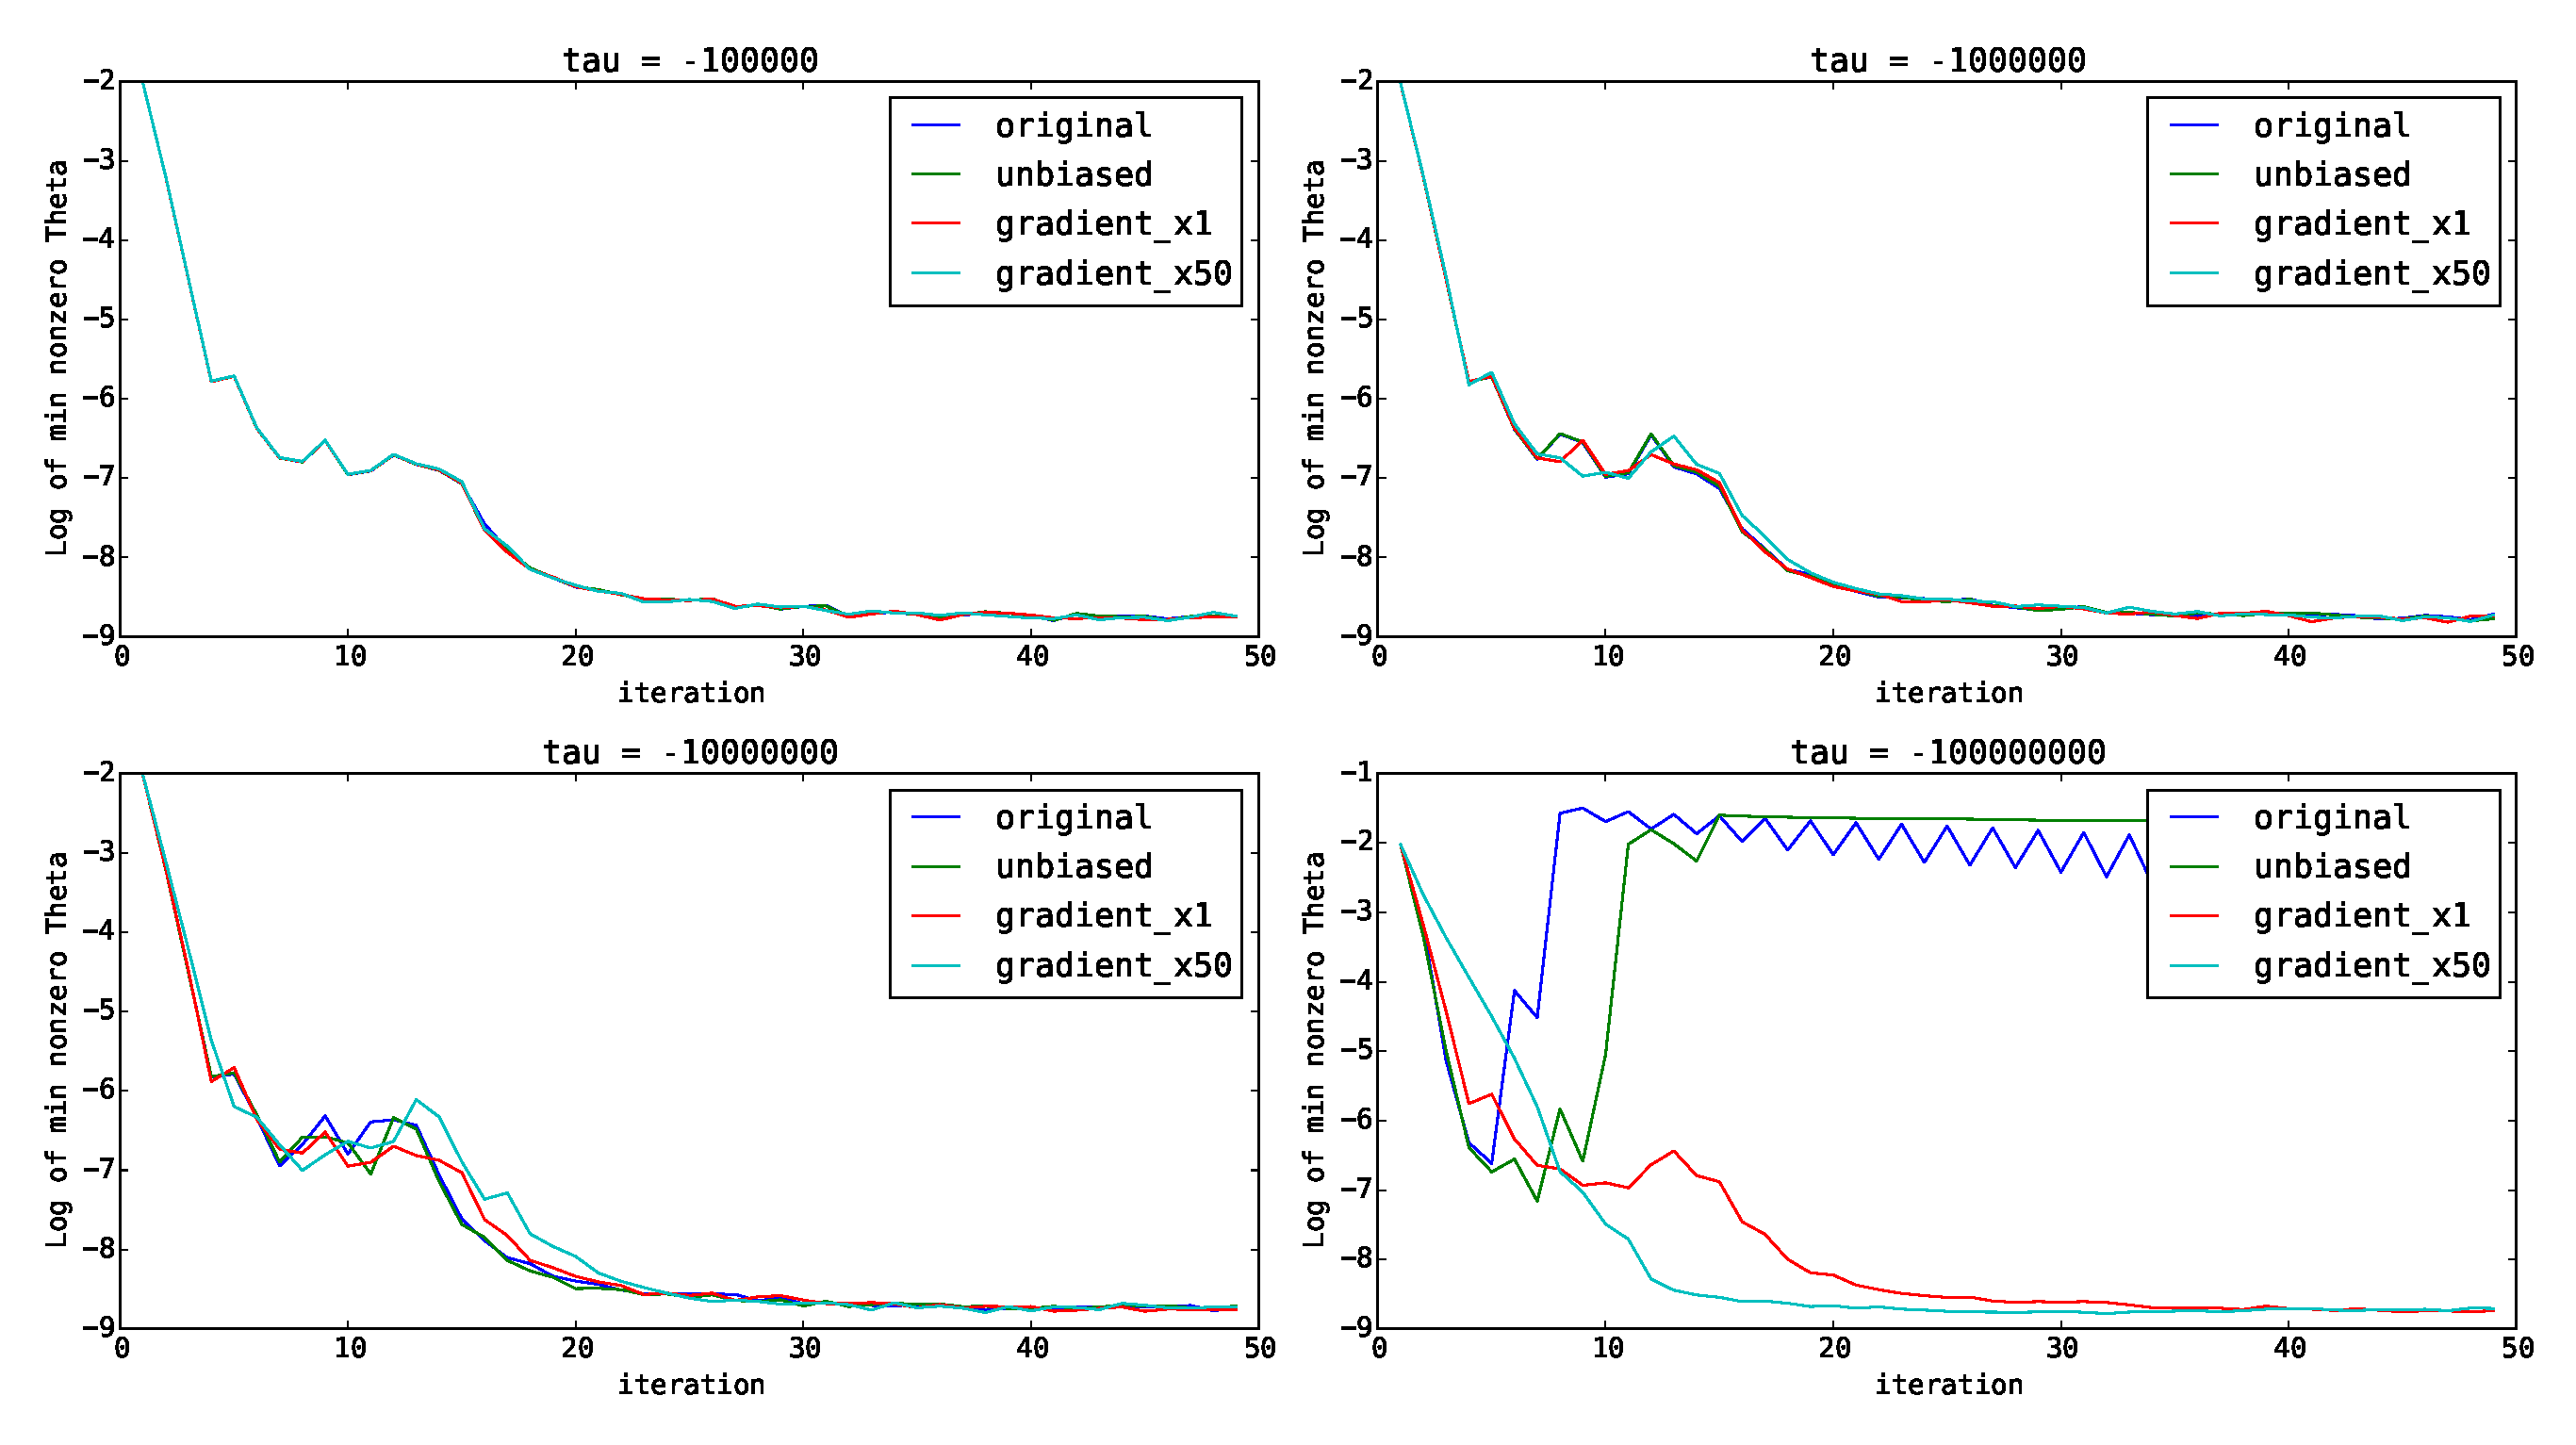
\includegraphics[width=1.0\linewidth]{pictures/topics_10_minTheta_values}
\end{figure}
\begin{figure}[H]
	\centering
	\caption{$|T| = 30$. Так же как и в предыдущих в графиках, дестабилизация происходит раньше из-за увеличения порядка значений $R$.}    
	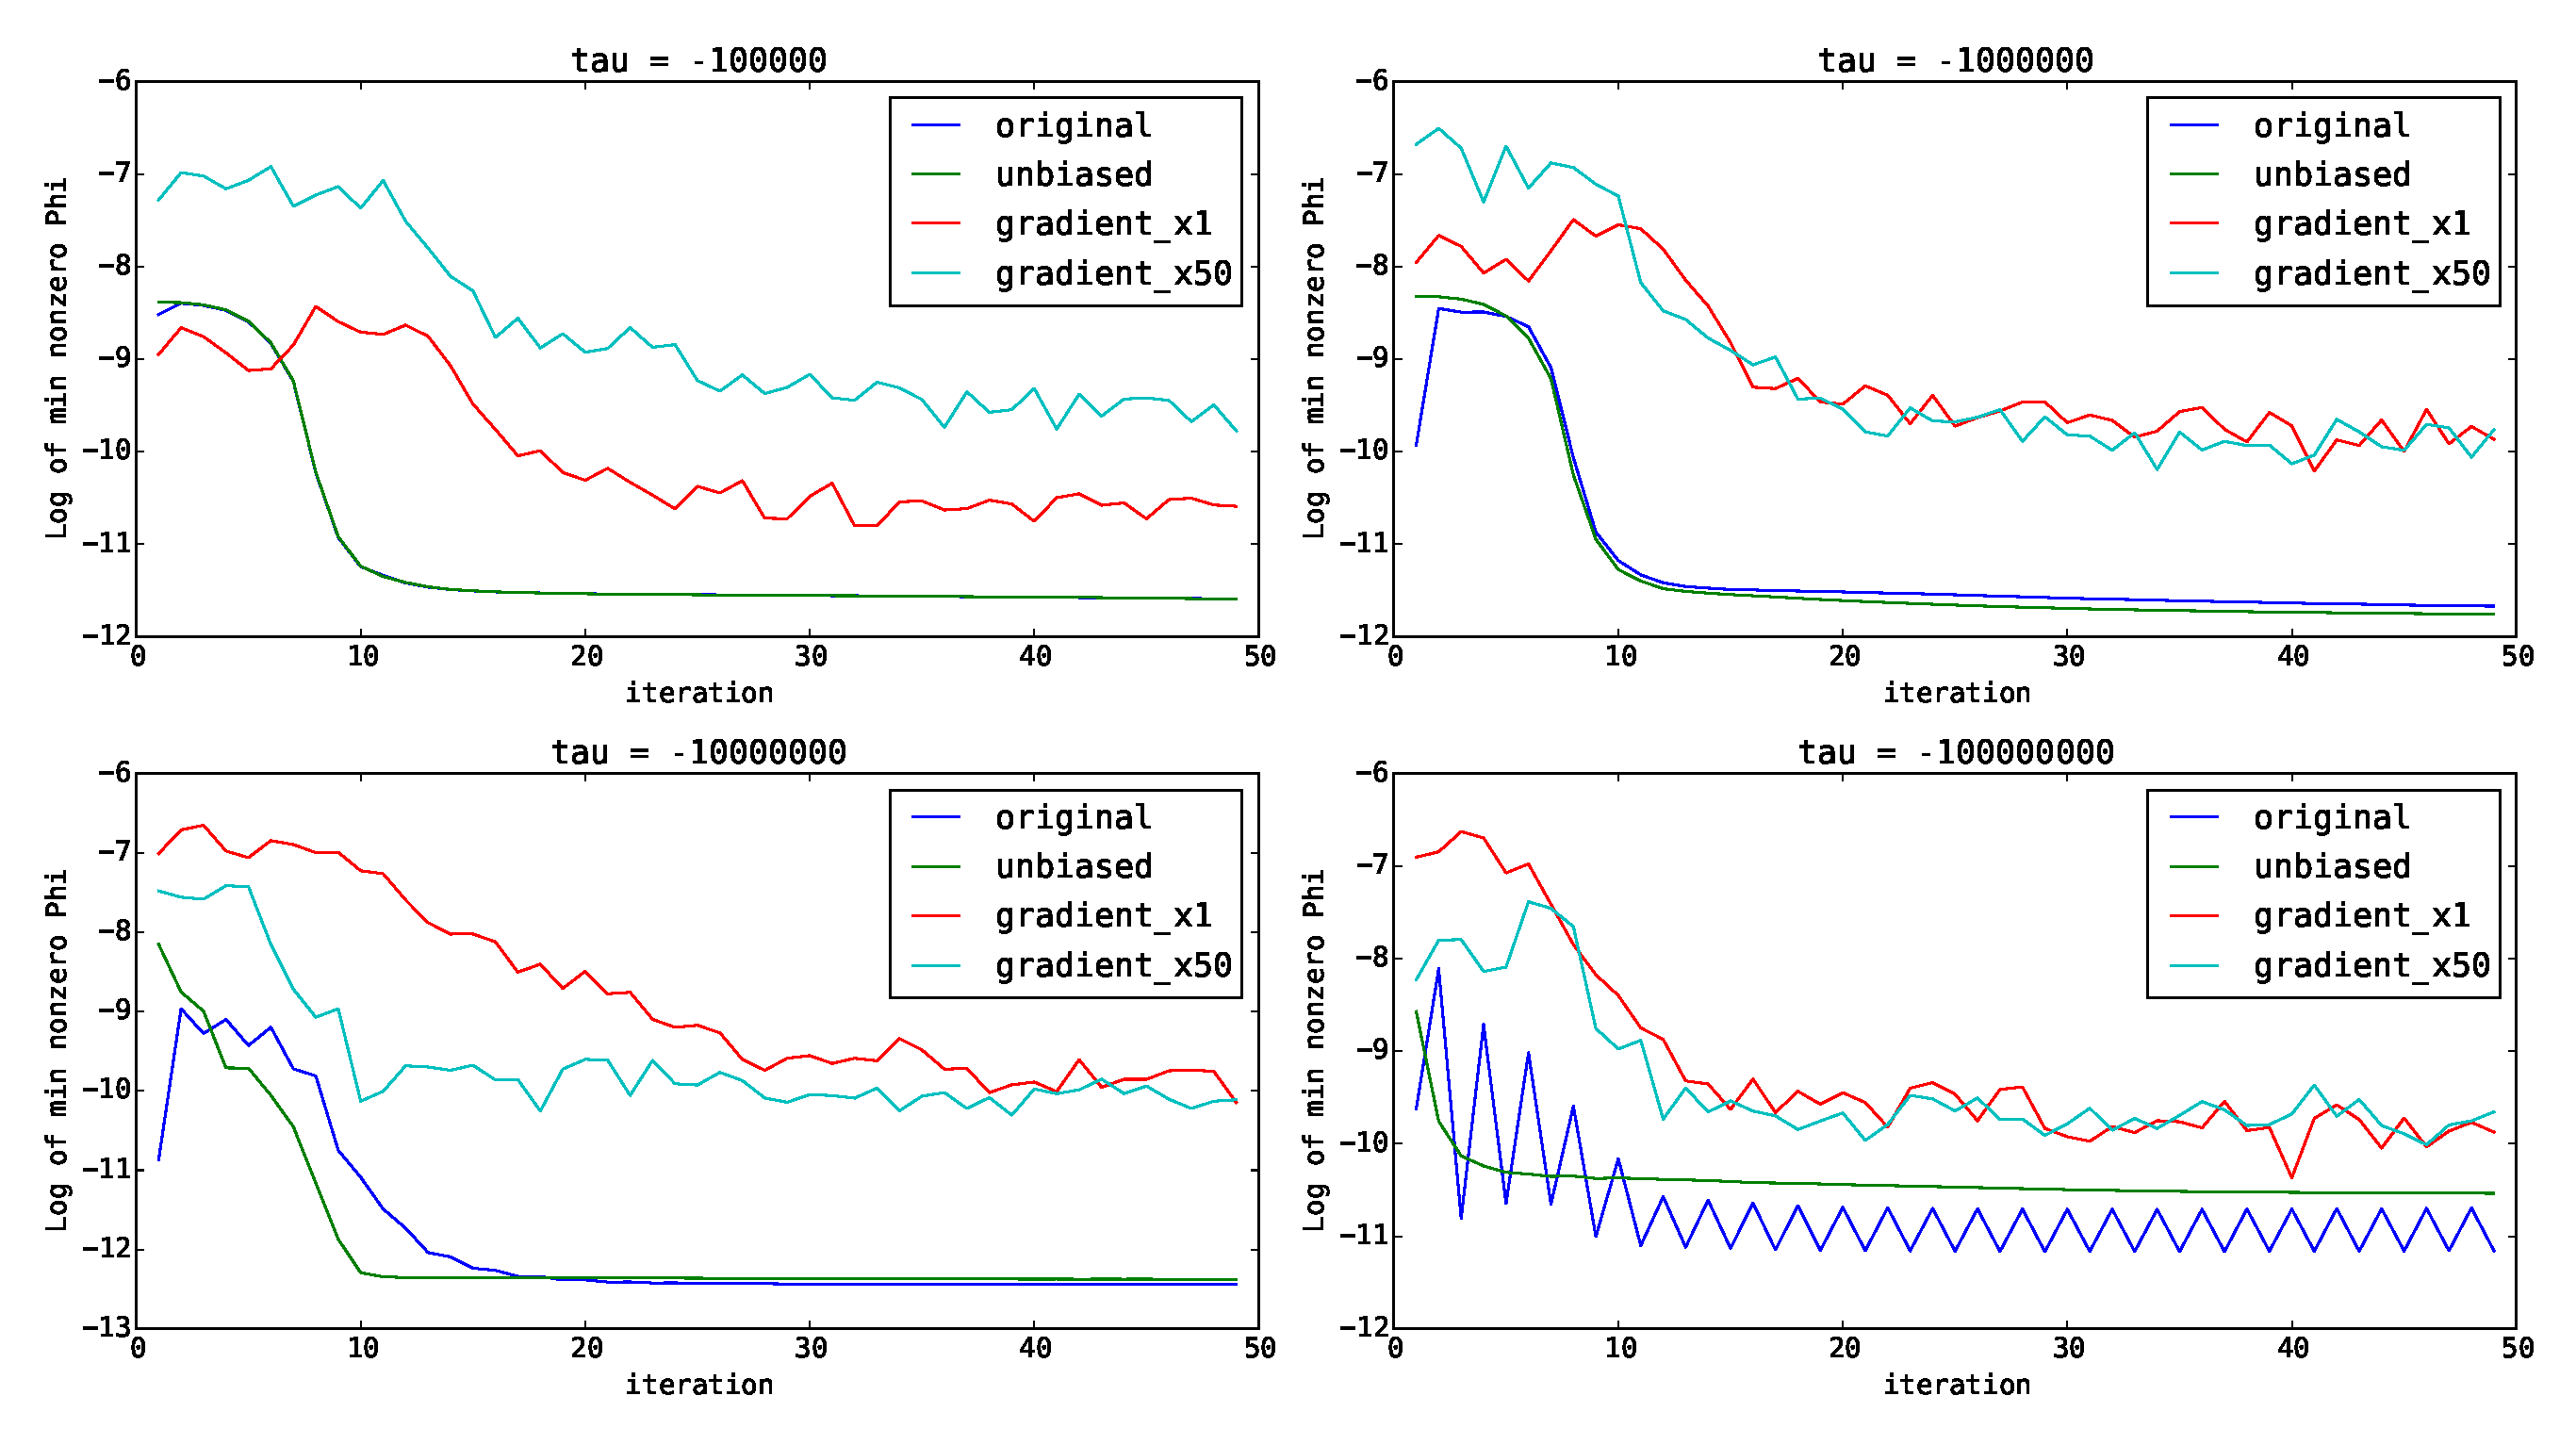
\includegraphics[width=1.0\linewidth]{pictures/topics_30_minPhi_values}
	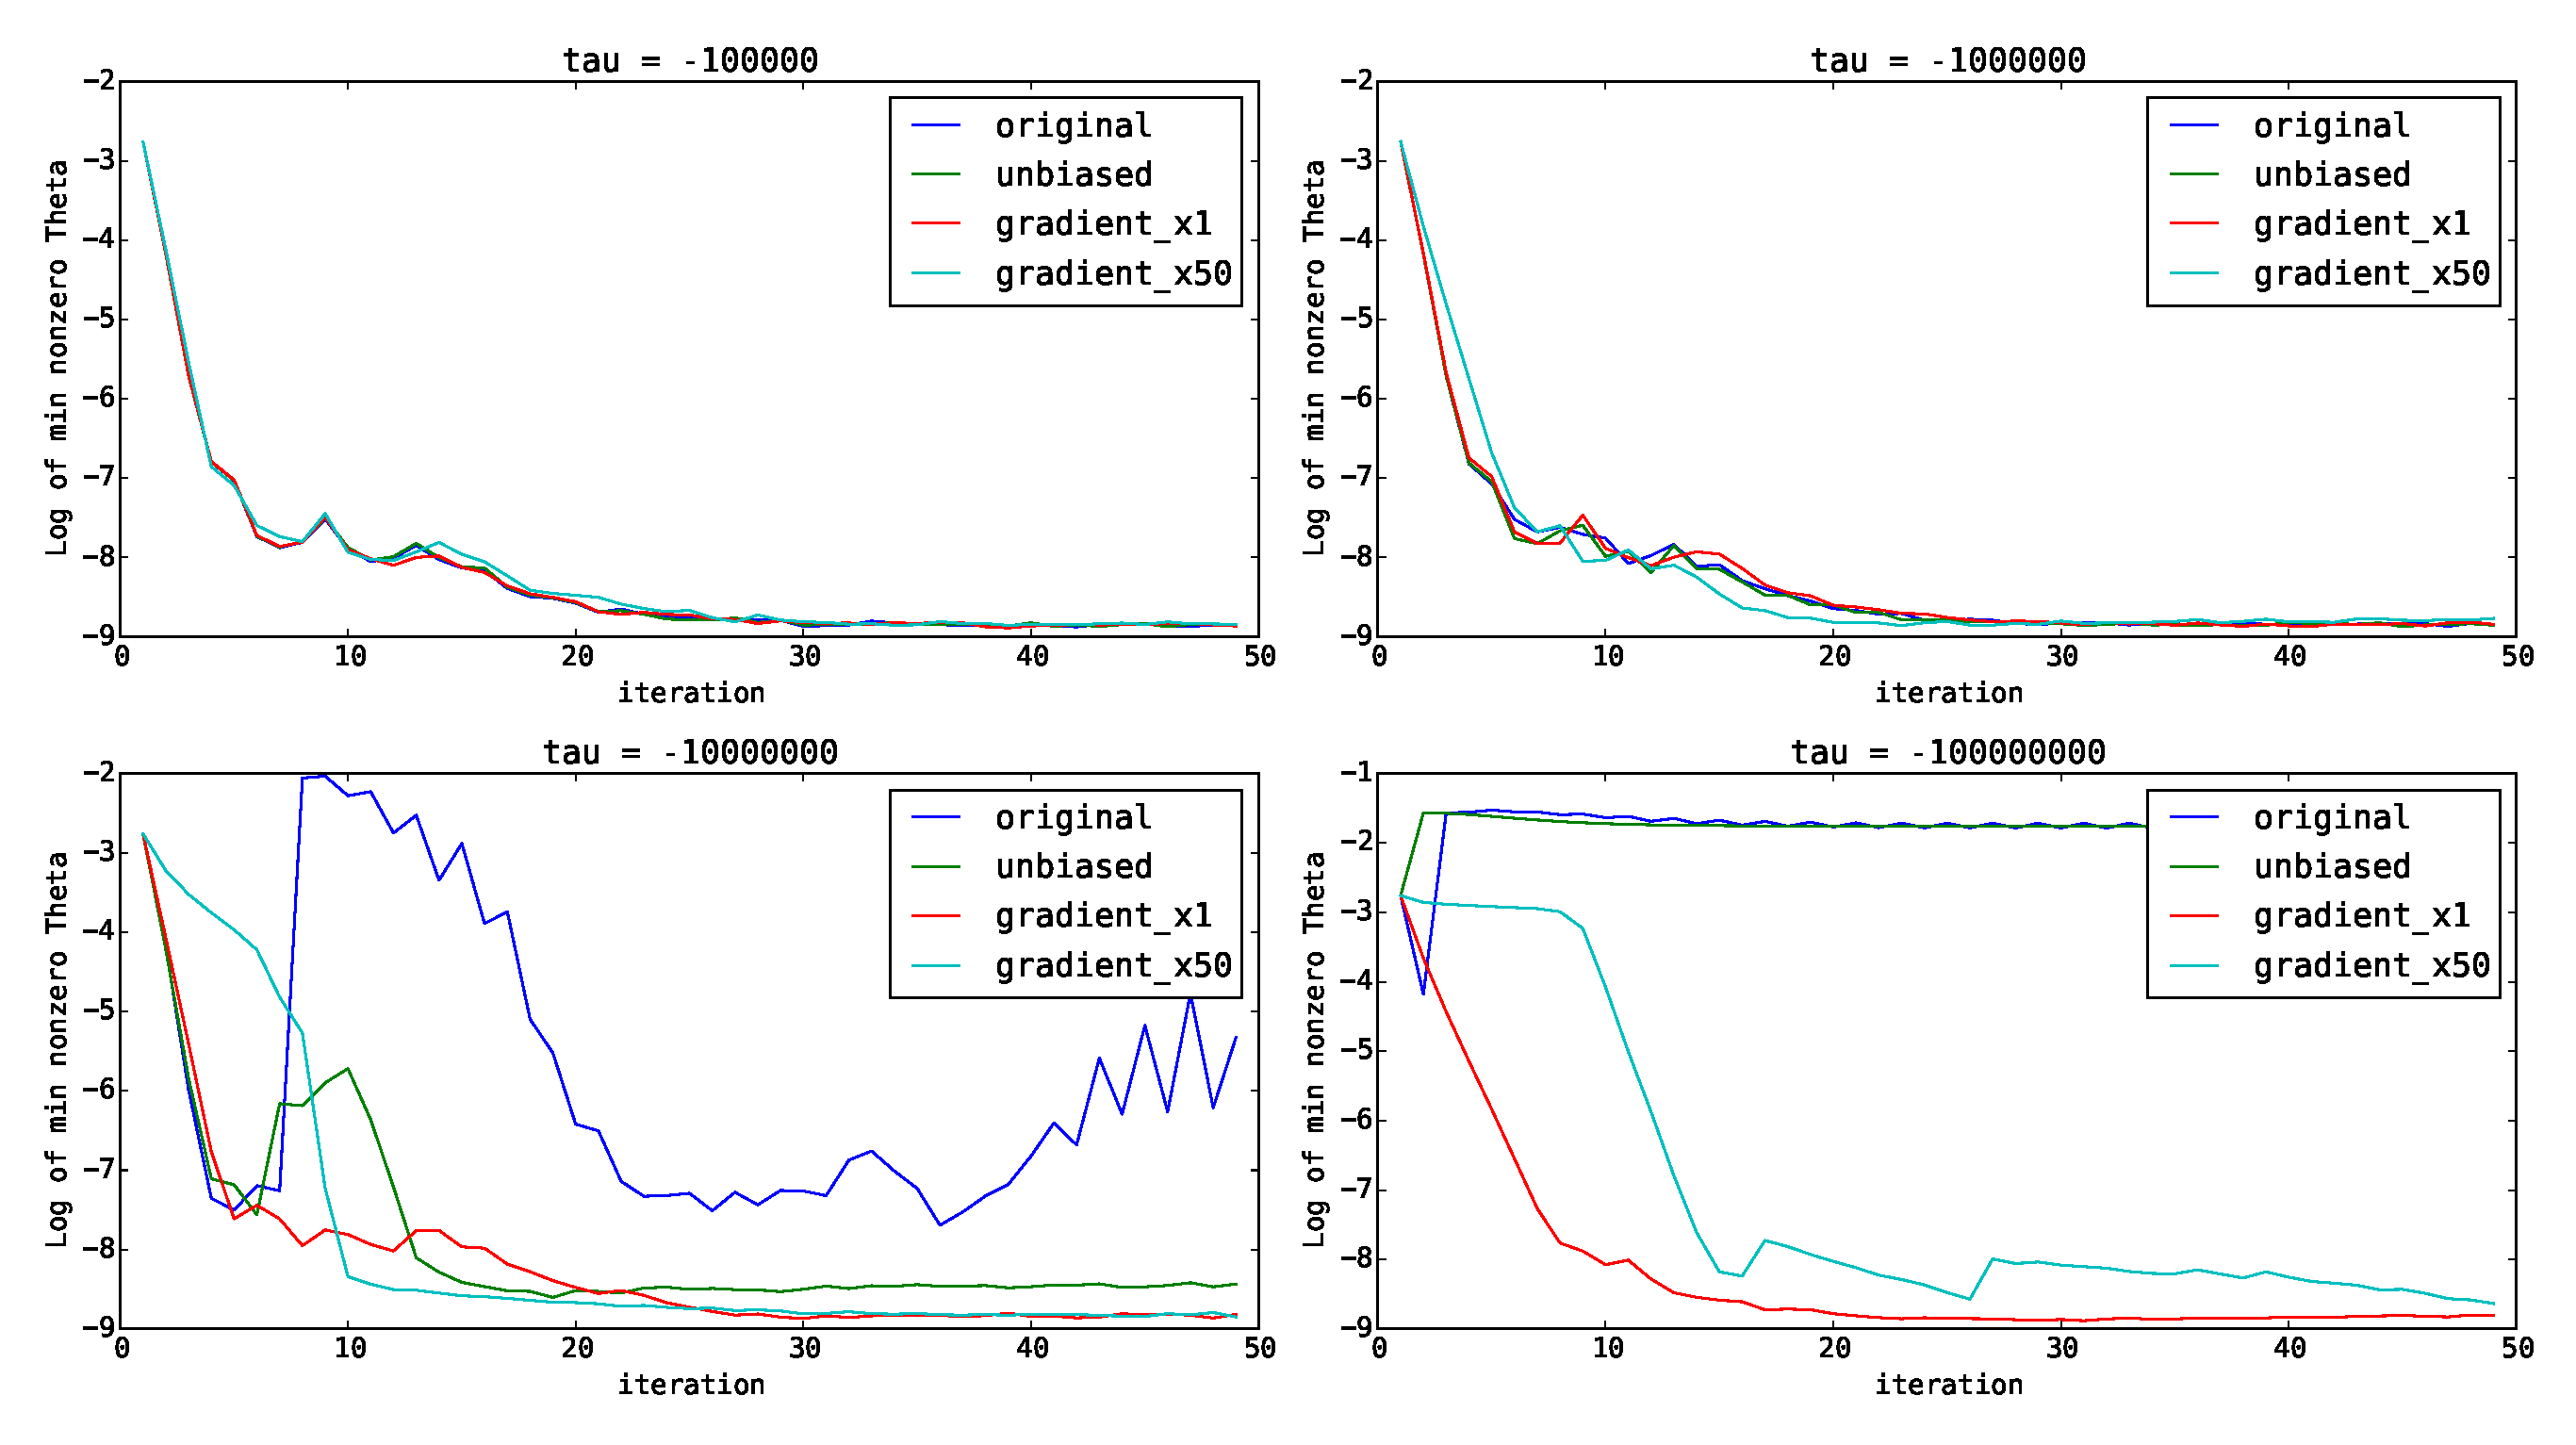
\includegraphics[width=1.0\linewidth]{pictures/topics_30_minTheta_values}
\end{figure}

Несмотря на то, что градиентные методы аккуратнее  зануляют элементы $\Phi$, они делают это заметно лучше -- значения существенно сильнее отделимы от нуля. Однако, в элементах $\Theta$ разницы нет, если не считать случая очень больших $|\tau|$, когда сильные множественные зануления привели к существенной отделимости параметров от нуля.
\subsubsection{Минимальный размер темы}
Второе важное свойство для сходимости алгоритма --- это сильная регулярность регуляризатора \ref{strongreg}. Фактически, важна отделимость от нуля знаменателя при нормировке в М-шаге. Именно эти значения  и были получены.
\begin{figure}[H]
	\centering
	\caption{$|T| = 3$.}    
	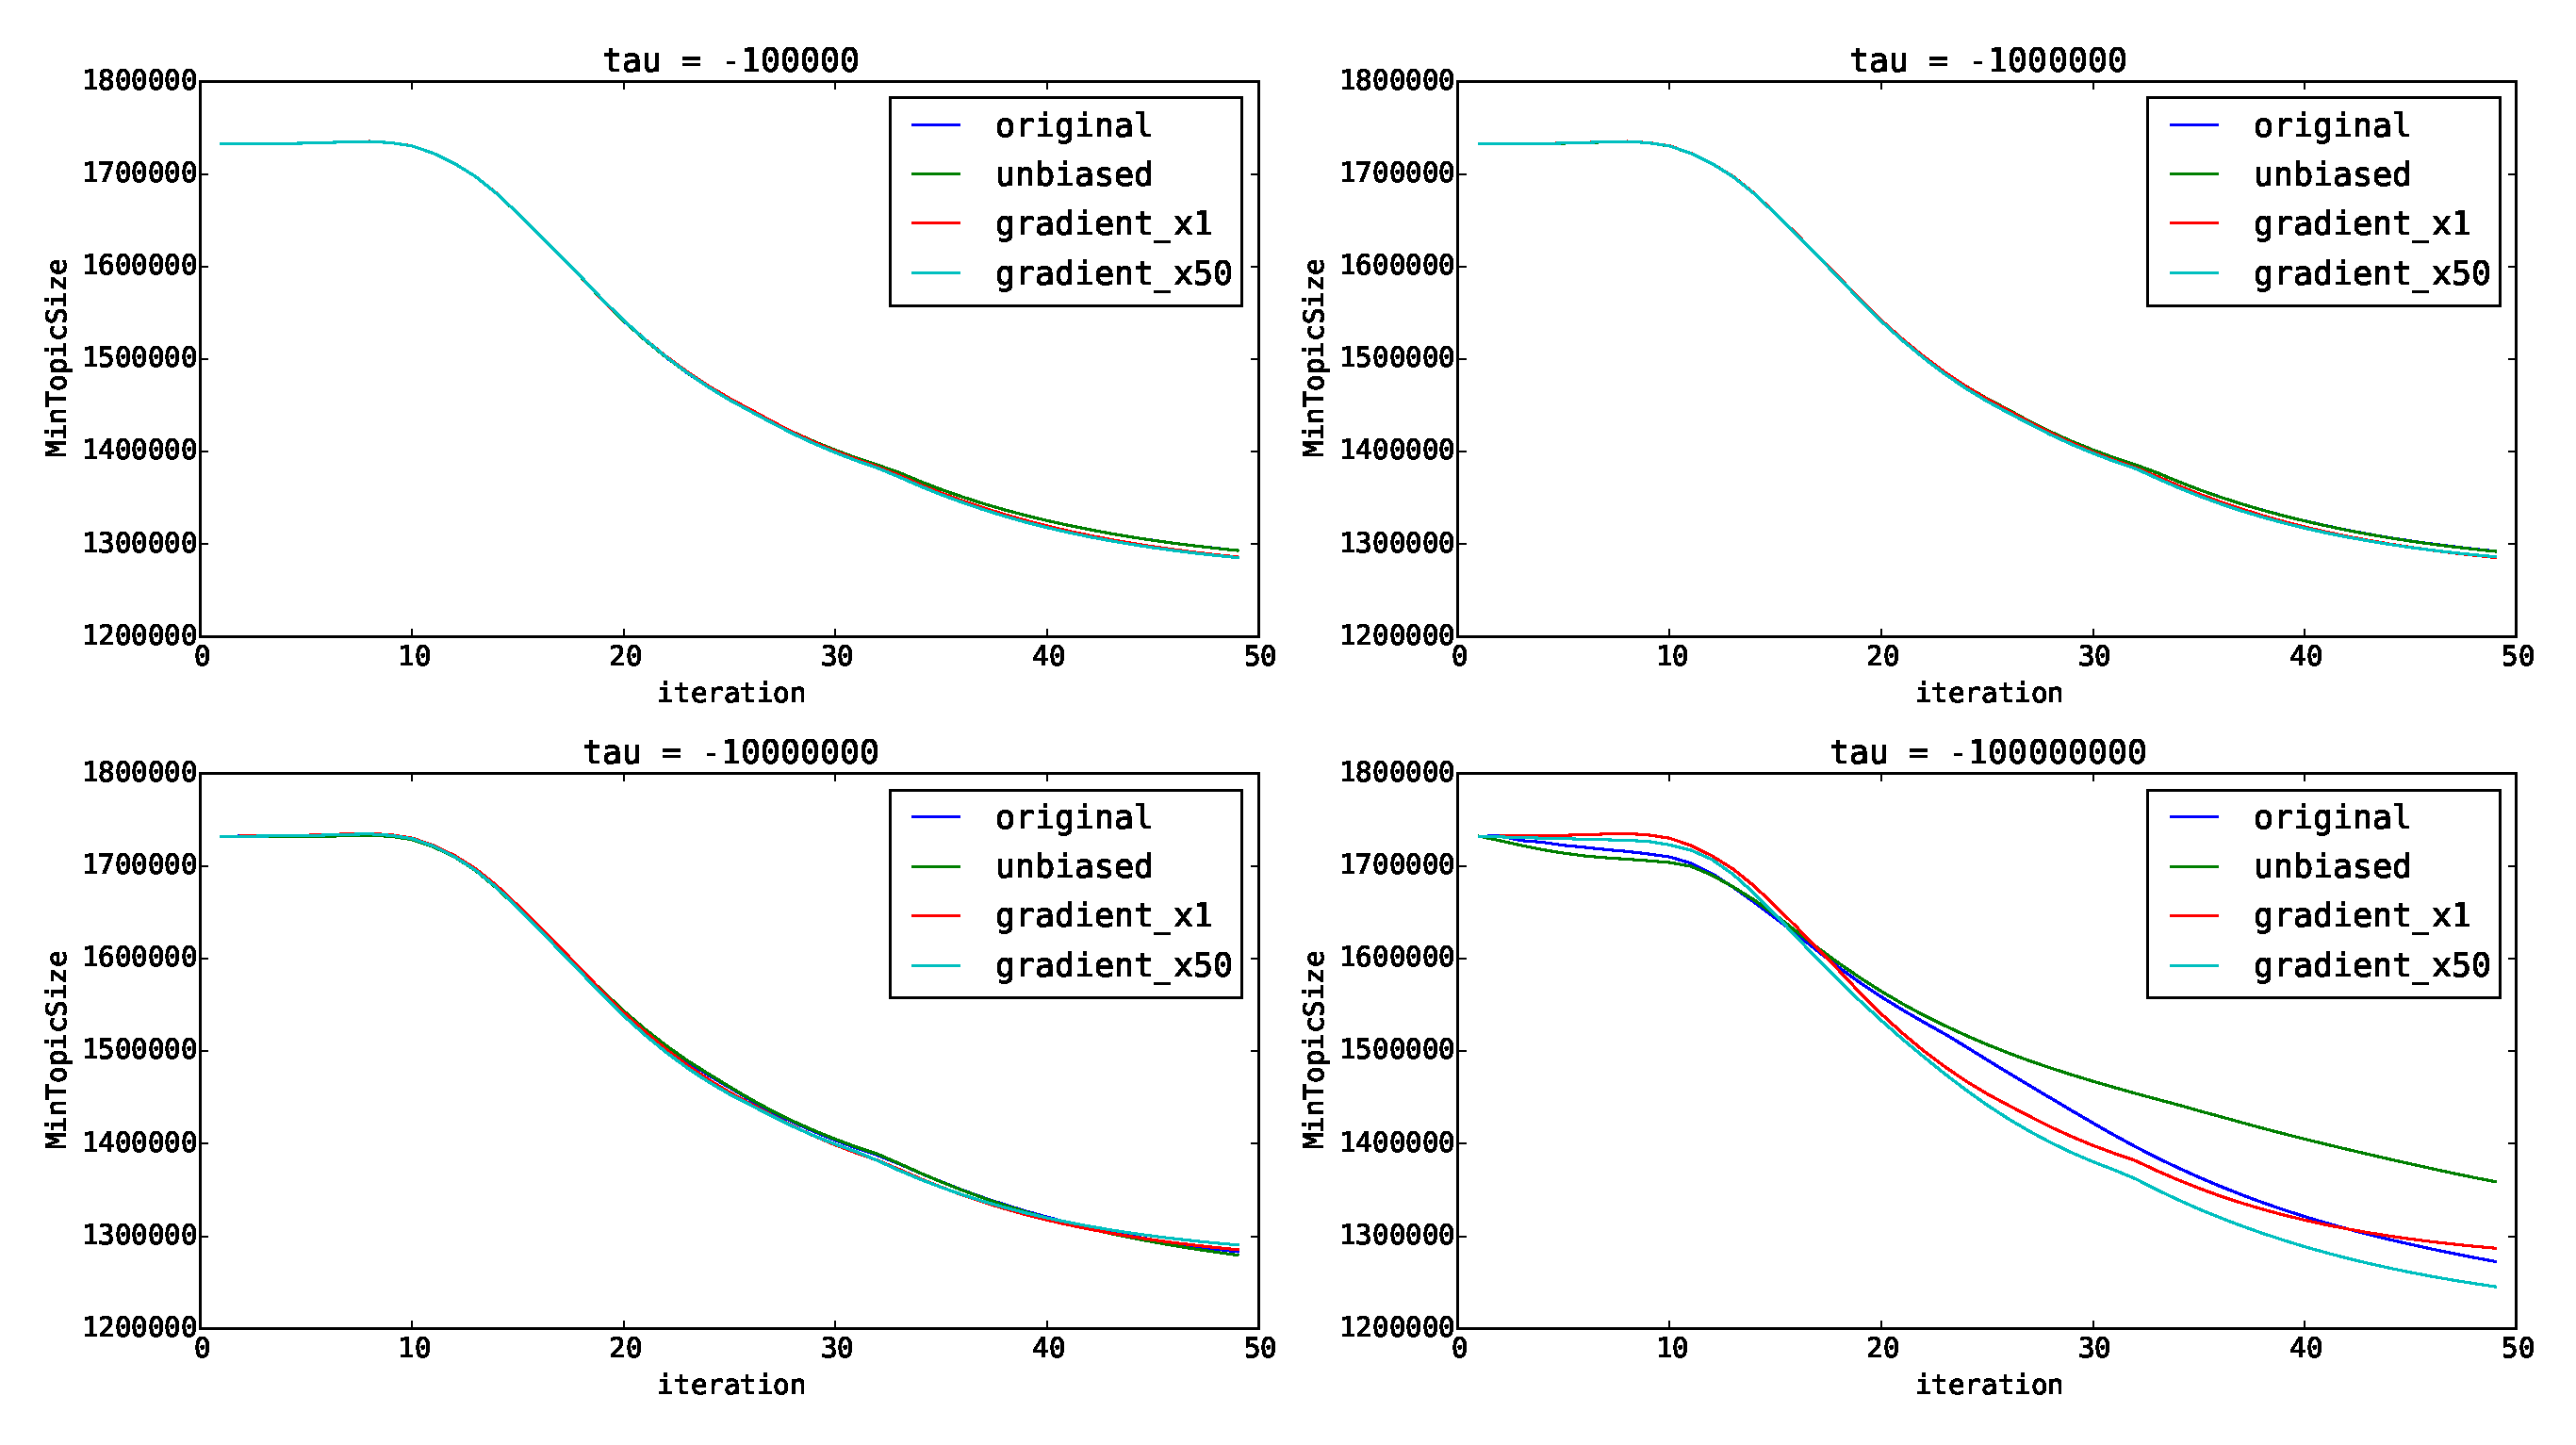
\includegraphics[width=1.0\linewidth]{pictures/topics_3_MinTopicSize}
\end{figure}

\begin{figure}[H]
	\centering
	\caption{$|T| = 10$.}    
	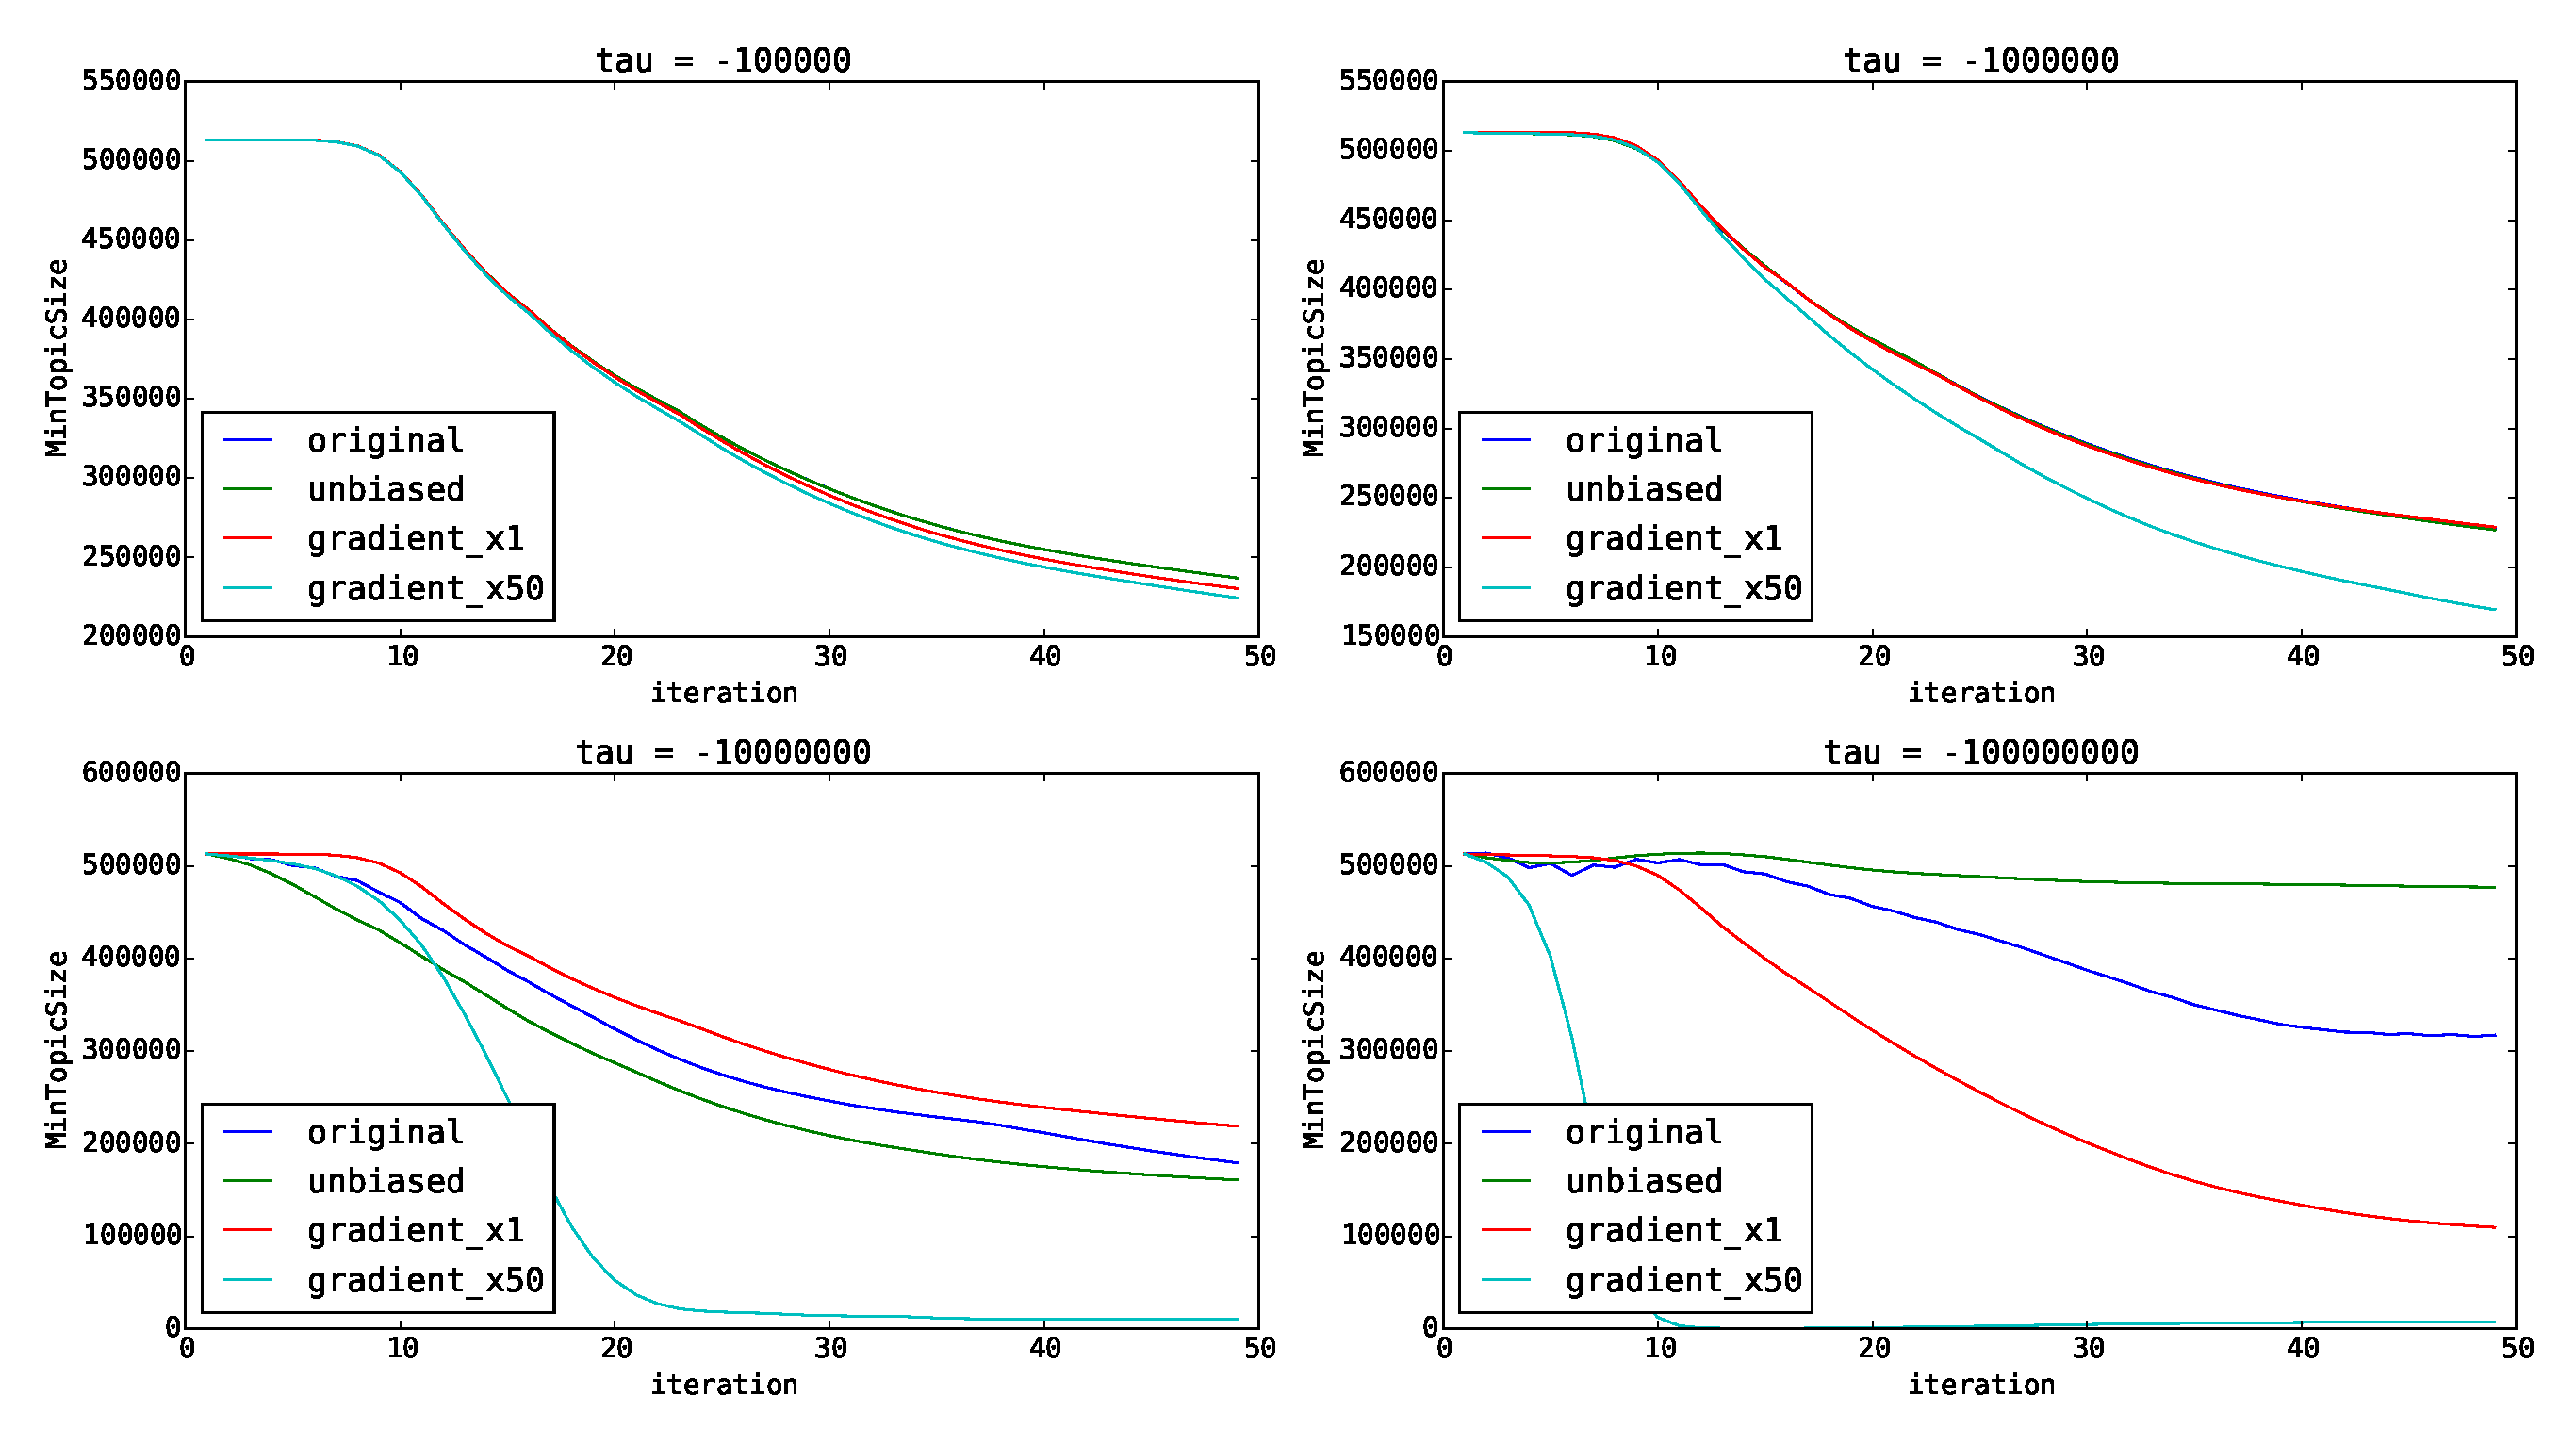
\includegraphics[width=1.0\linewidth]{pictures/topics_10_MinTopicSize}
\end{figure}

\begin{figure}[H]
	\centering
	\caption{$|T| = 30$.}    
	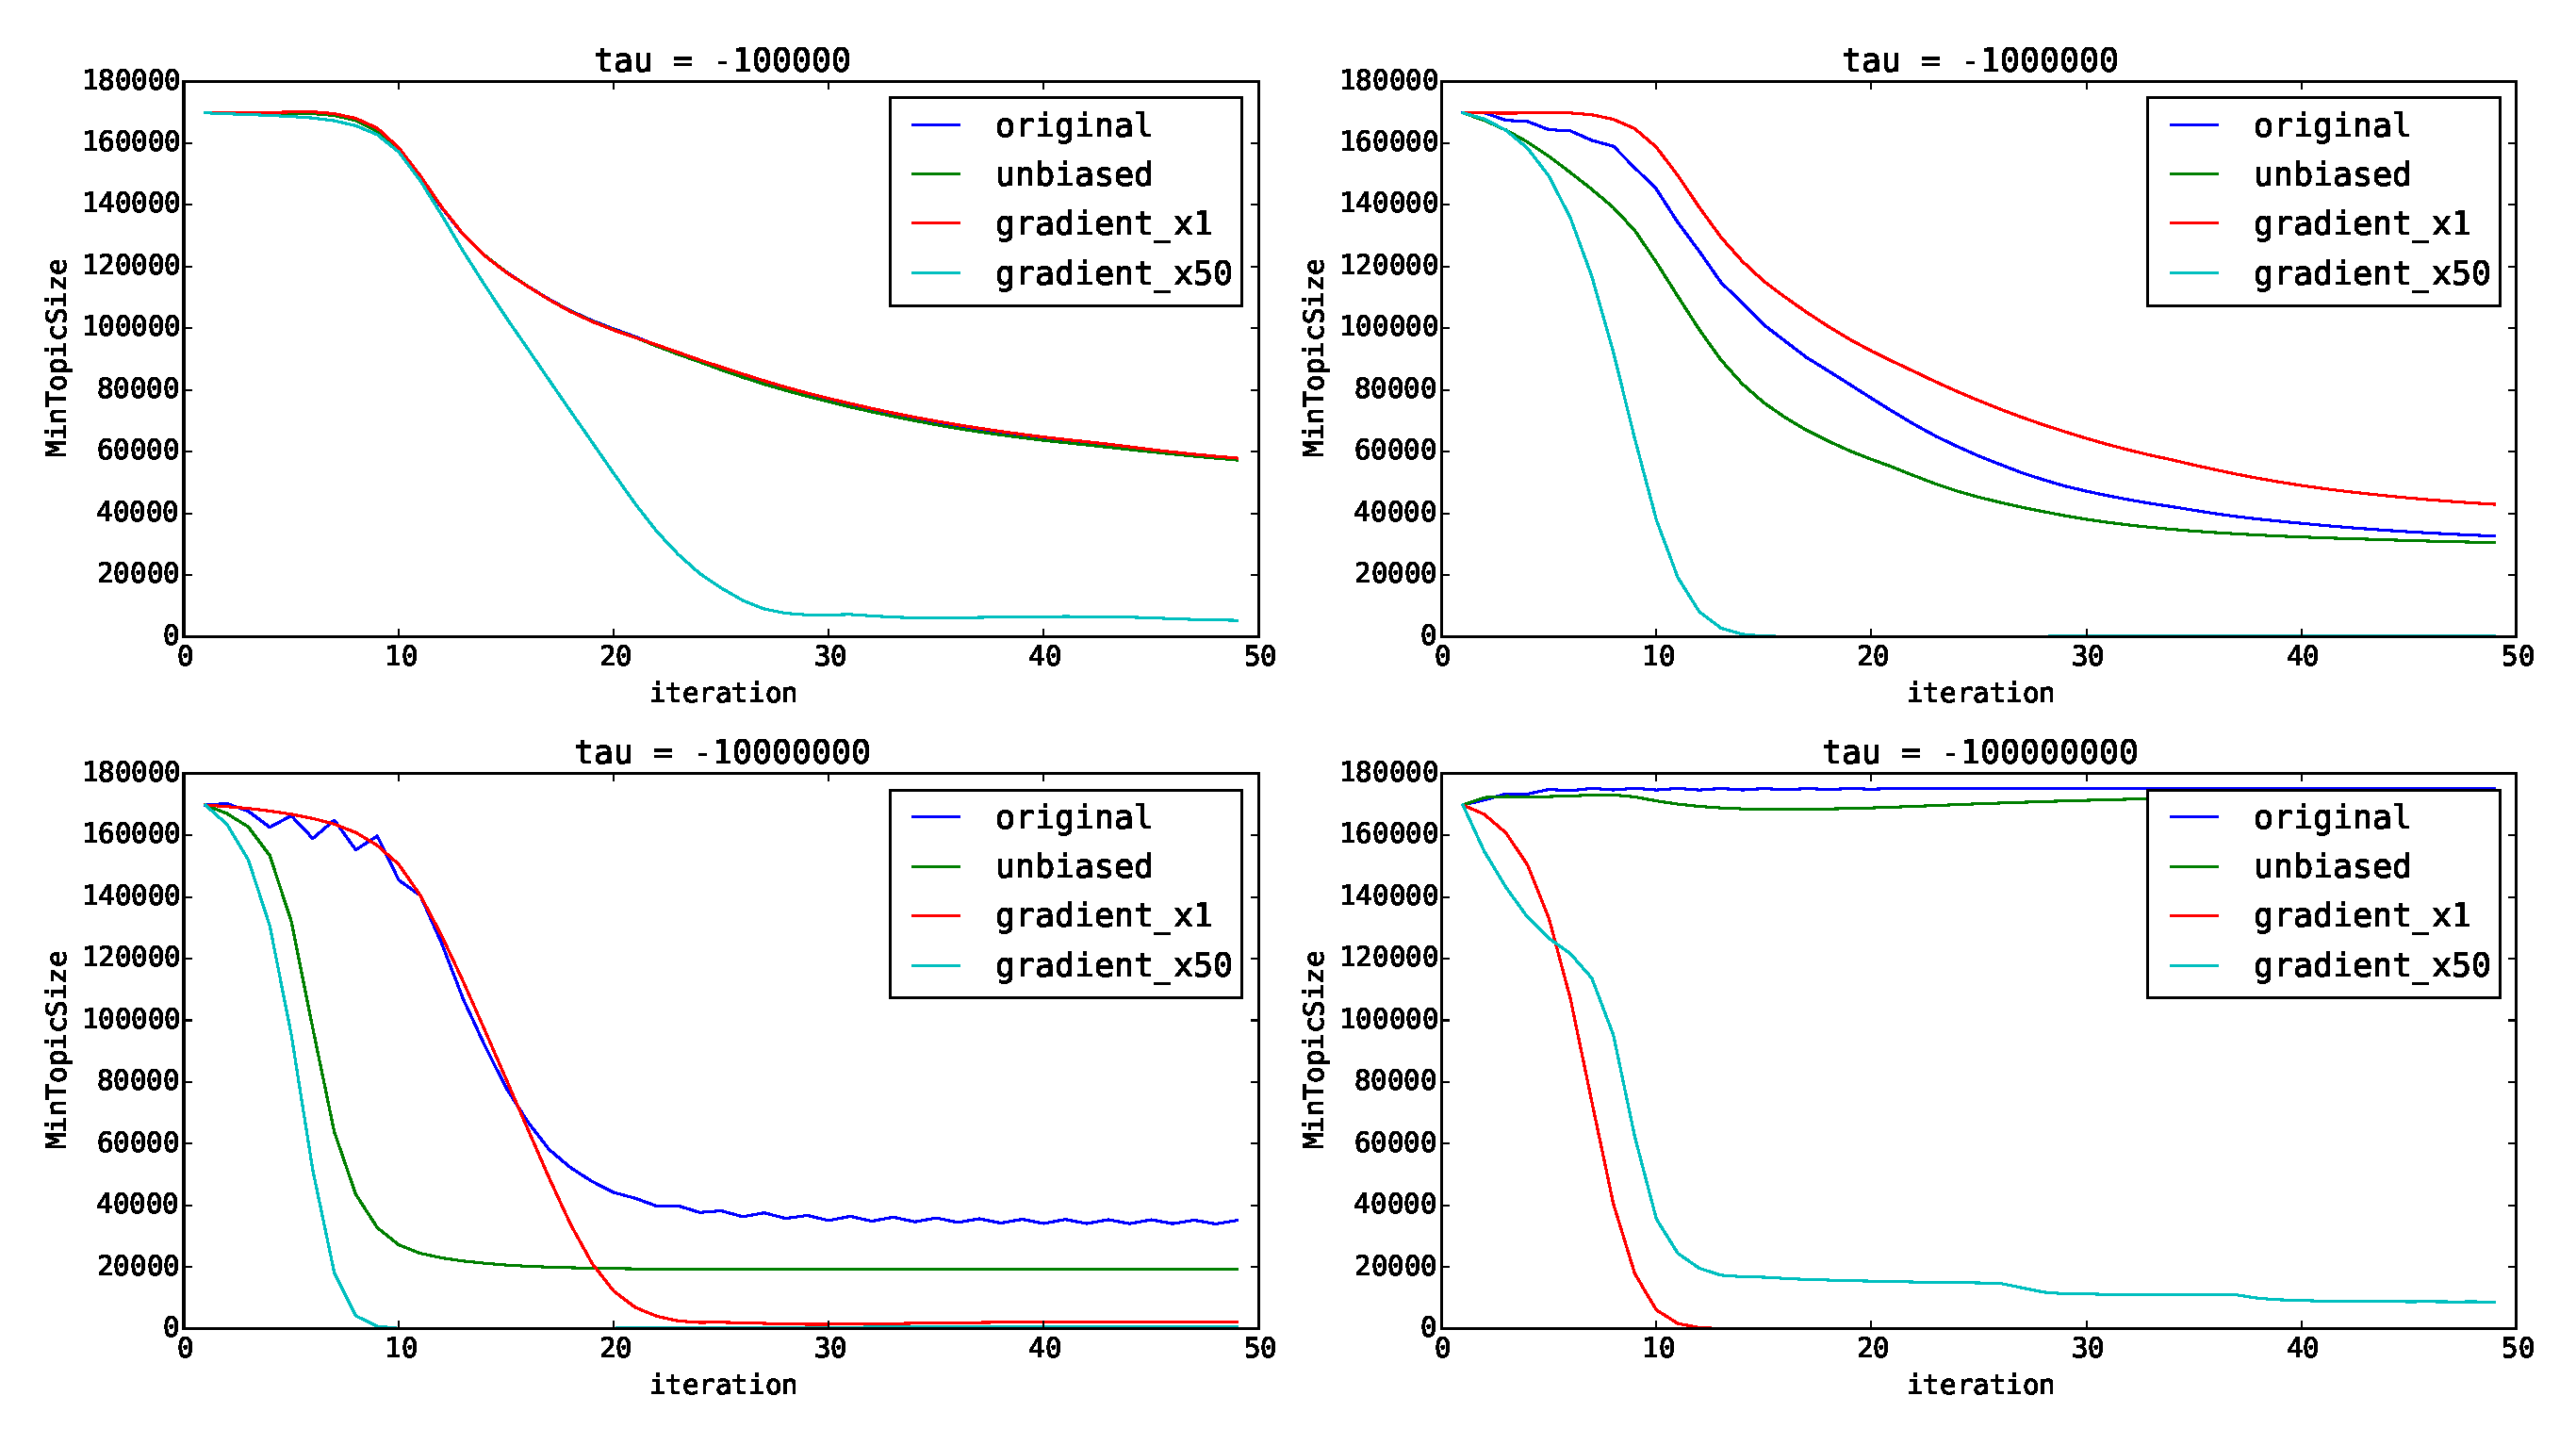
\includegraphics[width=1.0\linewidth]{pictures/topics_30_MinTopicSize}
\end{figure}

Значения становятся очень малыми, но отделимость от нуля сохраняется (просто отделено небольшой константой порядка 1, но на фоне 10000 это кажется нулём). 

Также видно, что градиентные методы более склонны к селекции тем. Отсюда можно сделать вывод, что градиентное направление обладает большей селективностью, чем стандартная формула. Также стоит отметить, что несмещённая модификация активнее отбирает темы чем стандартная формула.
\subsubsection{Итоги экспериментов}
На основании проведённых экспериментов можно сделать следующие выводы:
\begin{enumerate}
\item Предположения о $\varepsilon$-отделимости и сильной регулярности выполняются на практике, или могут легко гарантироваться за счёт реализации.
\item С точки зрения оптимизации $L + \tau R$ все рассмотренные формулы отличаются незначительно. Основное достоинтсво предложенных модификаций в этом плане --- это теоретические гарантии.
\item Есть эффект скачков значений функционалов на первых итерациях для стандартной формулы. Его можно избежать, если пользоваться несмещённой модификацией, для которой есть доказанное утверждение про увеличение $R$, что приводит к более гладкой траектории. Таким образом, данная модификация явно улучшает стандартную формулу.
\item Для градиентных поправок необходимо дополнительное исследование, чтобы понять как подбирать константу перед градиентом. Эксперименты показали наличие потенциала подобной модификации.
\end{enumerate}
\section{Заключение}
	Подведём краткое резюме данной работы. В вероятностном тематическом моделированиии существует подход ARTM, он предоставляет быстрый и очень гибкий функционал для оптимизации, легко адаптируемый под конкретную задачу. Основная его идея состоит в максимизации регуляризованного правдоподобия при помощи ЕМ-алгоритма. На практике предложенный алгоритм успешно сходился, однако, не было теоретического обоснования данной сходимости. Определение ограничений, при выполнении которых, можно гарантировать сходимость, было целью данной работы. Итерации алгоритма ARTM были проинтерпретированы как итерации GEM алгоритма, для которых условия сходимости хорошо изучены. Используя данные результаты, были найдены естественные ограничения на регуляризатор, выполнение которых достаточно просто проверить на практике. Пусть $k$ --- это номер итерации, тогда полученные условия можно сформулировать следующим образом:
\begin{enumerate}
\item Сохранение нуля регуляризатором.
\smallskip

$ n^k_{wt} = 0 \Rightarrow \phi^k_{wt} = 0$ , $n^k_{td} = 0 \Rightarrow \theta^k_{td} = 0$.
\item $\varepsilon$-отделимость от нуля элементов матриц $\Phi$ и $\Theta$.
\smallskip

$\exists \varepsilon>0\ \exists N\ \forall k > N\ \phi^k_{wt}, \theta^k_{td} \notin (0, \varepsilon)$. 
\item  Конечность логарифма правдоподобия на итерациях.
\smallskip

$ n_{dw}>0 \Rightarrow \forall k\ \exists t\colon p^k_{tdw} > 0$.
\item Отделимость от нуля знаменателя на М-шаге.
\smallskip

$\exists \delta >0\ \exists N\ \forall k > N \ \forall t\ \exists w\  n^k_{wt} + r^k_{wt} > \delta$ и аналогичное условие для $\theta$. 
\item Неуменьшение нижней оценки регуляризованного правдоподобия на итерациях.
\smallskip

$\exists N\ \forall k > N\colon\ \ Q^k (\phi^k, \theta^k)+ R(\Phi^k, \Theta^k) \geq Q^k(\phi^{k-1}, \theta^{k-1}) + R(\Phi^{k-1}, \Theta^{k-1})$, где $Q^k(\phi, \Theta) = \sum\limits_{t,d,w} p^k_{tdw} (\ln \phi_{wt} + \ln \theta_{td})$.
\end{enumerate}
Первое условие легко проверяется аналитически. Второе и третье условия можно обеспечить при реализации алгоритма. Четвёртое условие для матрицы $\Phi$ можно проинтерпретировать как критерий селекции тем. То есть, если значение становится меньше $\delta$, то зануляется вся строчка матрицы $\Phi$. С точки зрения реализации это эквивалентно просто удалению строчки в матрице и уменьшению числа тем. Для матрицы $\Theta$ выполнение данного условия можно достичь за счёт выбора $\tau$. Пятое условие должно быть обеспеченно за счёт правильного выбора регуляризационных добавок. Стандартный алгоритм предлагает использовать $r_{wt}^{k} = \tau \phi_{wt}^{k-1} \frac{\partial{R}}{\partial{\phi_{wt}}}(\phi_{wt^{k-1}}, \theta_{td}^{k-1})$ и $r_{td}^{k}=\tau  \theta_{td}^{k-1} \frac{\partial{R}}{\partial{\theta_{td}}}(\phi_{wt}^{k-1}, \theta_{td}^{k-1})$. Для данных формул не удалось получить хороших оценок, поэтому была рассмотрена следующая модификация: замена всех вхождений $\phi_{wt}$ и $\theta_{td}$ на их несмещённые оценки. То есть  $r_{wt}^k= \tau \frac{n^k_{wt}}{n^k_t}\frac{\partial{R}}{\partial{\phi_{wt}}}\bigl(\frac{n^k_{wt}}{n^k_t}, \frac{n^k_{td}}{n^k_d}\bigr)$ и $r_{td}^k= \tau \frac{n^k_{td}}{n^k_d}\frac{\partial{R}}{\partial{\theta_{td}}}\bigl(\frac{n^k_{wt}}{n^k_t}, \frac{n^k_{td}}{n^k_d}\bigr)$. Используя идею, что можно рассматривать функцию $R$ не как функцию от $\phi_{wt}$ и $\theta_{td}$, а как функцию от $n_{wt}$ и $n_{td}$, только с нормировкой аргументов, было получено, что на М-шаге происходит увеличение $R$, если взято не слишком большое $\tau$. Также была предложена идея использовать вычисленный градиент $R$ в качестве регуляризационных добавок на М-шаге: $r^k_{wt} = \tau A_t \bigl[{\frac{\partial{R}}{\partial{\phi_{wt}}} - \sum\limits_u \phi_{ut} \frac{\partial{R}}{\partial{\phi_{ut}}} }\bigr] \bigl(\frac{n^k_{wt}}{n^k_t}, \frac{n^k_{td}}{n^k_d}\bigr)$ и $r^k_{td} = \tau B_d \bigl[ {\frac{\partial{R}}{\partial{\theta_{td}}} - \sum\limits_s \theta_{sd} \frac{\partial{R}}{\partial{\theta_{sd}}} }\bigr] \bigl(\frac{n^k_{wt}}{n^k_t}, \frac{n^k_{td}}{n^k_d}\bigr)$. Определение формул для $A_t$ и $B_d$ в данной работе не производилось, для экспериментов использовались самые наивные варианты.

Был проведён эксперимент, в котором сравнивались три возможных формулы М-шага. Предложенные модификации показали небольшое улучшение по сравнению со стандартными формулами. Также был замечен следующий эффект: при достаточно больших $\tau$ наблюдаются скачки в функционалах для стандартной формулы М-шага, это свидетельствует в пользу того, что не получится теоретически доказать неуменьшение $R$ на М-шаге для стандартной формулы.

\subsection{Результаты, выносимые на защиту}
\begin{enumerate}
\item Условия для сходимости ЕМ-алгоритма ARTM, легко проверяемые и обеспечиваемые при реализациии.
\item Две модификации формул М-шага ЕМ-алгоритма, улучшающие сходимость без увеличения вычислительной сложности.
\item Оценки изменения значений регуляризатора и логарифма правдоподобия на итерациях для предложенных модификаций.
\end{enumerate}
\newpage

\bibliographystyle{gost71s}
\bibliography{Articles}

\end{document}